%#####################################################################################################################
% Datei	: BillysPayback.tex
% Autor	: Byron Worms
%#####################################################################################################################
% Dokumenteinstellungen
\documentclass[bibliography=totoc,listof=totoc,version=first,a4paper,12pt,numbers=noendperiod,appendixprefix=true,
oneside,headsepline,footsepline,openright]{scrbook}

% Seitenr�nder festlegen
\usepackage[top=2.5cm,bottom=3.0cm,left=3.0cm,right=2.0cm]{geometry}

% Umlaute etc..
\usepackage[latin1]{inputenc}
\usepackage[T1]{fontenc}

% Bilder unterst�tzen
\usepackage[]{graphicx}

% Farben unterst�tzen
\usepackage{xcolor}
\usepackage{color}
\usepackage{colortbl}

% Bibliothek f�r das Quellenverzeichnisse
\usepackage[style=numeric,backend=biber,sorting=none]{biblatex}
\addbibresource{Literaturverzeichnis.bib}
%\renewcommand{\bibfont}{\small} --> finde ich zu klein

%defernumbers=true --> Das hat zu Problemen mit der Nummerierung gef�hrt!

% Verweise auf Title
\usepackage{titleref}

% Sprachunterst�tzung (Letzte Sprache wird als Richtlinie genutzt!)
\usepackage[english,ngerman]{babel} 
\usepackage{csquotes}

% Symbolunterst�tzung wie €
\usepackage{textcomp}

% Abk�rzungsverzeichnis unterst�tzen
\usepackage[printonlyused]{acronym}

% Anhang unterst�tzen
\usepackage[titletoc]{appendix}

% Erweiterte Fu�noten unterst�tzen
\usepackage[hang]{footmisc}
\setlength{\footnotemargin}{1em}

% Unterst�tzung mehrzeiliger Kommentare
\usepackage{comment}

% Folgende Objekte kapitel�bergreifend nummieren: Tabelle, Abbildungen, Fu�noten
\usepackage{chngcntr} 
\counterwithout{footnote}{chapter}

% Erweiterte Tabellen unterst�tzen
\usepackage{booktabs}
\usepackage{tabularx}
\usepackage{tabulary}
\usepackage{longtable,tabu}
\usepackage{array}
\usepackage{multicol}

% Mathematische Operationen in {} Ausdr�cken erlauben (z.B. {\linewidth-4cm})
\usepackage{calc}

% "float" Positionierung unterst�tzen
\usepackage{scrhack}
\usepackage{float}

% Erweiterte Aufzählungen unterst�tzen
\usepackage{enumitem}

% Erweiterte Tabellenlinien unterst�tzen
\usepackage{hhline,float}

% Rotationen unterst�tzen
\usepackage{rotating}

% Erweiterte Symbole unterst�tzen
\usepackage{bbding} 
\usepackage{dingbat}
\usepackage{wasysym}

\usepackage{url}

% Querformat unterst�tzen
\usepackage{pdflscape}

% Verweise in PDF-Datein aktivieren (muss das letzte importierte Package sein!)
\usepackage[colorlinks=false]{hyperref}

% Tabellen werden nicht von Latex neupositioniert
\restylefloat{table}

% Bilder werden nicht von Latex neupositioniert
\restylefloat{figure}

% PDF Version 1.6 erzwingen
\pdfminorversion=6

% Kompression ausschalten (hyperref setzt das Level auf 9!)
\pdfcompresslevel=9

% Verschiebungen und Formattierungen des Modus "twoside" aufheben
\raggedbottom

% Informationen zu dem Dokument
\newcommand{\thetitle}{Billy's Payback: Rising of the Fruits}
\newcommand{\theauthorr}{Billy's Payback}
\author{\theauthorr}
\title{\thetitle}

% Funktionen f�r das Ausblenden/Einblenden von nummerierten Überschriften im Inhaltsverzeichnis.
% Kapitel, Sektion, Untersektion
\newcommand{\hideInContents}{\addtocontents{toc}{\protect\setcounter{tocdepth}{-1}}}
\newcommand{\showInContents}{\addtocontents{toc}{\protect\setcounter{tocdepth}{2}}}

% Fake "Tabitem" erzeugen
\newcommand{\tabitem}{~~\llap{\textbullet}~~}

% Diverse Hilfsfunktionen
\newcommand{\bold}{\normalfont \bfseries}
\newcommand{\boldtext}[1]{{\normalfont \bfseries {#1}}}

% Funktion zum L�schen der Seite. Der Befehl unterscheidet automatisch zwischen einseitig und zweiseitig!
\newcommand{\myclearpage}{\if@twoside \cleardoublepage \else \clearpage \fi }

% Entfernt die Kopfzeile von automatisch generierten Leerseiten
\makeatletter
\def\cleardoublepage{\cleardoubleemptypage}
\makeatother

%---------------------------------------------------------------------------------------------------------------------
% Einstiegspunkt
%---------------------------------------------------------------------------------------------------------------------
\begin{document}
	\myclearpage
	\begingroup
		\renewcommand*{\chapterpagestyle}{empty}
		\pagestyle{empty}
		%#####################################################################################################################
% Datei	: Sperrvermerk.tex
% Autor	: Byron Worms
%#####################################################################################################################
\begin{center}
\huge
\vspace*{\fill}
\boldtext{Platzhalter f�r das Deckblatt}
\vspace*{\fill}
\end{center}						% Titelseite einbinden
		\cleardoubleemptypage
		%%#####################################################################################################################
% Datei	: Abstrakt.tex
% Autor	: Byron Worms
%#####################################################################################################################
\let\raggedsection\centering
\section*{Kurzfassung}
Englische Kurzfassung
\selectlanguage{english}
\section*{\abstractname}
\let\raggedsection\raggedright
Deutsche Kurzfassung
\selectlanguage{ngerman}					% Kurzfassung einbinden
		%\cleardoubleemptypage		
		\pagenumbering{Roman}									% R�mische Seiternummerierung	
		\tableofcontents 										% Inhaltsverzeichnis generieren
%		\include{Inhalt/ABK}									% Abk�rzungsverzeichnis einbinden
		\listoffigures{}										% Abbildungsverzeichnis generieren
%		\listoftables{}											% Tabellenverzeichnis generieren
	\myclearpage
	\endgroup
	
	\cleardoublepage  											
	\pagenumbering{arabic}										% Arabische Seiternummerierung
	
%................................................................
% Ab hier den eigentlichen Inhalt einf�gen
	%#####################################################################################################################
% Datei	: Einleitung.tex
% Autor	: Ulrike Uderhardt
%#####################################################################################################################
\chapter{Einleitung}
\label{chap:einleitung}


%Schon vor Jahrzehnten haben Computerspiele in die Kinder- und Wohnzimmer unserer Welt Einzug genommen und sind heutzutage kaum noch wegzudenken. Dabei dienen Computerspiele haupts�chlich der Unterhaltung der Spieler. Die Vielfalt an unterschiedlichen Spiel-Genre ist enorm. Besonders beliebt sind storybasierte Spiele, bei denen der Spieler und seine Handlungen durch die Geschichte gelenkt werden und sich so die ganze Story nach und nach aufbaut. Dabei erf�hrt der Spieler meist sehr deutlich die Einschr�nkung, den Verlauf der Geschichte nicht beeinflussen zu k�nnen. Allerdings ist diese Begrenzung der Entscheidungsfreiheit unvermeidbar, da der Entwickler ein bestimmtes Geschehen verfolgen will. Der Spieler muss zum Beispiel Gegenst�nde aufsammeln, Gegner besiegen und bestimmten Wegen folgen, um am Ende ans Ziel zu gelangen. Ohne diese bestimmten Handlungen geht es in der Geschichte nicht weiter. Mit dieser Arbeit soll ein Prototyp eines 2,5D-Jump-and-Run-Spiels entstehen, der dem Spieler die angesprochene begrenzte Entscheidungsfreiheit suggeriert. Um dem Spieler solch ein Gef�hl der freien Wahl vorzut�uschen, soll eine Analyse seines Verhaltens erfolgen und darauf basierende Manipulationen den festgelegten Verlauf verschleiern. Teilweise stammen diese aus dem Bereich der Psychologie, teilweise aus bereits vorhandenen Computerspielen, die diese Thematik auch aufgreifen. Bisher finden Manipulationen jedoch gr��tenteils in 3D-Spielen eine breite Anwendung. In 2,5D-Spielen und speziell in Jump-and-Runs wurde dieser Bereich erst wenig behandelt. Auch sind wissenschaftliche Untersuchungen zum Thema Manipulationen im Allgemeinen bisher eher rar, insbesondere in Bezug auf dieses Spiel-Genre.

Schon vor Jahrzehnten haben Computerspiele in die Kinder- und Wohnzimmer unserer Welt Einzug genommen und sind heutzutage kaum noch wegzudenken und dienen haupts�chlich Unterhaltung der Spieler. Dabei baut die Handlung der meisten Spiele auf einer vom Entwickler vorgegebenen Geschichte auf. Dies f�hrt jedoch dazu, dass der Spieler  meist sehr deutlich die Einschr�nkung erf�hrt den Verlauf der Geschichte nicht beeinflussen zu k�nnen. Allerdings ist diese Begrenzung der Entscheidungsfreiheit unvermeidbar, damit ein bestimmtes Geschehen verfolgen werden kann. Der Spieler muss zum Beispiel Gegenst�nde aufsammeln, Gegner besiegen und bestimmten Wegen nachgehen, um am Ende ans Ziel zu gelangen. Ohne diese Handlungen geht es in der Geschichte nicht weiter. Dieser Effekt kann jedoch mit Hilfe von Manipulationen abgeschw�cht werden, indem versucht wird den Spieler unterbewusst auf die gew�nschten Wege zu f�hren, ohne dass dieser davon etwas mitbekommt. Dies wird in der Praxis von 3D-Spielen bereits erfolgreich angewandt. Im Bereich der 2,5D Jump and Runs sind Manipulationsstrategien jedoch bisher noch nicht allzu h�ufig anzutreffen und auch an wissenschaftlichen Untersuchungen zum Thema Spielermanipulation mangelt es bisher. An diesem Punkt soll daher die aktuelle Arbeit ansetzen.

\section{Zielsetzung}
\label{sec:einleitung zielsetzung}

Ziel der Arbeit ist die Beantwortung der Frage, inwiefern es m�glich ist die Manipulationen, die bereits in 3D-Spielen Verwendung finden, auf 2,5D Jump and Runs zu �bertragen. Zu diesem Zweck soll ein prototypisches Spiel dieses Genres entwickelt werden, das eine Evaluierung der ausgew�hlten Manipulationen m�glich macht. Diese erfolgt dabei mit Hilfe von Probanden, die den Prototypen spielen und anschlie�end eine Reihe von Fragen zu ihrem Spielerlebnis beantworten sollen. Um die Manipulationen unter realistischeren Bedingungen testen zu k�nnen, soll der Prototyp au�erdem um eine m�glichst geschlossene Geschichte herum aufgebaut werden.\\
Des Weiteren wird der Erfolg des Prototypen anhand bestimmter Erfolgskriterien gemessen, deren Erf�llung ebenfalls anhand der abschlie�enden Evaluierung �berpr�ft werden soll. So sollen mindestens 70\% der Spieler den Spa�faktor mit gut bewerten, um herauszufinden, ob der Prototyp im Rahmen seiner M�glichkeit dem Hauptziel eines Spiels gerecht werden konnte.  Dar�ber hinaus l�sst sich nur von einer potenziell erfolgreichen Anwendung bzw. �bertragung der Manipulationen sprechen, wenn sich die Probanden mindestens in 80\% der F�lle f�r den gew�nschten Weg entscheiden und zumindest 66\% der Spieler einen alternativen Weg bzw. ein alternatives Ende f�r m�glich halten.


%Der Erfolg des Prototypen soll anhand von drei Kriterien gemessen werden, welche mit Hilfe einer anschlie�enden Evaluierung �berpr�ft werden sollen. Dazu ist ein Fragebogen auszuarbeiten, den die Probanden nach dem Spielen gereicht bekommen. Anhand einer Skala von \grqq trifft voll und ganz zu\grqq \ bis \grqq trifft �berhaupt nicht zu\grqq \ k�nnen die Probanden unterschiedliche Kriterien bewerten. Als Ziel sollen zun�chst 70\% der Spieler den Spa�faktor mit \grqq trifft zu\grqq \ oder besser beurteilen. Als n�chstes sollen sich die Spieler in mindestens 80\% der F�lle f�r den gew�nschten Weg entscheiden. Und 66\% der Spieler sollen einen alternativen Weg bzw. ein alternatives Ende f�r m�glich halten.
%Das Ziel der Arbeit ist somit die Evaluierung der ausgew�hlten Manipulationen anhand eines Prototypen, um herauszufinden, inwiefern diese innerhalb eines 2,5D-Jump-and-Runs Erfolg haben. Um die Manipulationen unter realistischeren Bedingungen testen zu k�nnen, soll eine m�glichst geschlossene Geschichte im Prototypen entwickelt werden.



%
% Nachfolgende Sektionen nicht im Inhaltsverzeichnis anzeigen lassen!
\hideInContents
%
%................................................................
% Hier die Sektionen f�r die Einleitung

%................................................................
%
% Die kommenden Kapitel, Sektionen und Untersektionen wieder im Inhaltsverzeichnis anzeigen
\showInContents						% Einleitung einbinden
	%#####################################################################################################################
% Datei	: Grundlagen.tex
% Autor	: Dominique Kasper
%#####################################################################################################################

\chapter{Grundlagen}
\label{chap:grundlagen}

%................................................................
\section{Manipulation}
\label{sec:manipulation}

%Ausstehende Quellen:
%Manipulation und Selbstt�uschung, Rainer Sachse {RSachseManipulationSelbsttaeuschung}

Um eine geeignete Auswahl an Manipulationen f�r den Spielprototypen treffen zu k�nnen, ist es zun�chst einmal notwendig die theoretischen Grundlagen der Manipulation sowie verschiedene Manipulationsstrategien zu kennen und zu verstehen. Aus diesem Grund soll hier sowohl transparentes und intransparentes Handeln als auch positive bzw. negative Manipulation und deren Folgen erl�utert werden. Anschlie�end erfolgt au�erdem eine Beschreibung m�glicher Manipulationsstrategien, aus denen sp�ter Manipulationen f�r den Prototypen abgeleitet werden (siehe Abschnitt \ref{sec:konzept manipulationen}).\\
Dar�ber hinaus sind diese Kenntnisse auch f�r die Auswahl der relevanten Spielereigenschaften von Nutzen.

\subsection{Transparentes und intransparentes Handeln}
\label{subsec:transparentes und intransparentes handeln}

Wenn zwei Personen (oder im Fall dieser Arbeit der Spieler und das Spiel) miteinander interagieren, wird dies als \textit{interaktionelle Handlung} bezeichnet. Dabei verfolgt jeder der beiden Interaktionspartner mit seinem Handeln eine bestimmte Absicht, d.h. er will damit ein bestimmtes Verhalten beim jeweils Anderen erreichen. Allerdings kann er auf zwei verschiedene Art und Weisen seine Absicht in eine Handlung umsetzen\cite{RSachseManipulationSelbsttaeuschung}

\begin{enumerate}
	\item Die Absicht kann durch sein Handeln erkennbar werden.
	\item Die Absicht kann verschleiert werden.
\end{enumerate}

\subsubsection{Transparentes Handeln}

Wird die Absicht durch das Handeln einer Person erkennbar, wird dies als \textit{transparentes Handeln} bezeichnet. Bei dieser Art des Handelns, kann der Gegen�ber selbst entscheiden, ob er der Absicht der Person entspricht oder nicht. Er hat somit echte Entscheidungsfreiheit, da er sich auf die wahre Absicht der Handlung einstellen kann. Ein Beispiel hierf�r w�re "Ich m�chte, dass du dich um mich k�mmerst.". Aussagen wie "Wenn sich doch jetzt nur jemand um mich k�mmern w�rde ...", wo der Interaktionspartner also zwischen den Zeilen lesen muss, werden zwar auch noch zu transparentem Handeln gez�hlt, k�nnen jedoch nicht mehr als v�llig transparent betrachtet werden, da hier ein zus�tzlicher Aufwand notwendig ist, um die Absicht zu entschl�sseln.\cite{RSachseManipulationSelbsttaeuschung}

\subsubsection{Intransparentes Handeln}

Wird die wahre Absicht jedoch verschleiert, handelt es sich um \textit{intransparentes Handeln}. In diesem Fall ist es sogar notwendig dem Gegen�ber eine glaubhafte, falsche Absicht f�r das eigene Handeln zu liefern und zwar eine, die er mit hoher Wahrscheinlichkeit auch akzeptiert. Welche Absicht das ist, ist wiederum von der Pers�nlichkeit des Interaktionspartners abh�ngig. Ist er beispielsweise jemand, der dazu neigt schnell Mitleid zu empfinden, ist es sinnvoll das Handeln mit einem schlechten Befinden zu begr�nden. So w�re es eine M�glichkeit zu sagen "Mir geht es heute wirklich schlecht, k�mmere dich bitte um mich.". Die Abh�ngigkeit des Erfolges einer Manipulation von den Eigenschaften des Gegen�bers wird in Abschnitt \ref{sec:konzept spielereigenschaften} im Bezug auf die Spielereigenschaften noch von Bedeutung sein. Durch dieses Hinwegt�uschen �ber die wahren Gr�nde des Handeln wird der Interaktionspartner jedoch auch seiner Entscheidungsfreiheit beraubt, denn da er nun die eigentliche Absicht nicht kennt, hat er nicht die M�glichkeit sich daf�r oder dagegen zu entscheiden. Dar�ber hinaus sind gut erdachte, falsche Absichten meist sehr zwingend, womit er sich verpflichtet f�hlt, diesen auch nachzugeben.\cite{RSachseManipulationSelbsttaeuschung}

\subsection{Definition der Manipulation}
\label{subsec:definition manipulation}

Auf der Grundlage des zuvor behandelten transparenten und intransparenten Handelns, l�sst sich nun gut der Begriff der Manipulation definieren. So hat diese laut Rainer Sachse drei wesentliche Eigenschaften\cite{RSachseManipulationSelbsttaeuschung}:

\begin{itemize}
	\item Intransparentes Handeln
	\item Veranlassung des Interaktionspartners zu einer Handlung, die er ohne Manipulation nicht ausf�hren w�rde
	\item Einschr�nkung der Entscheidungsm�glichkeiten des Interaktionspartners durch die T�uschung hinsichtlich der wahren Handlungsgr�nde
\end{itemize}

Dar�ber hinaus nimmt er eine Unterscheidung der Manipulationen hinsichtlich der Folgen des durch die Manipulation erfolgten Handelns f�r die manipulierte Person vor. Diese sollen im Folgenden erl�utert werden.

\subsection{Positive Manipulation}
\label{subsec:positive manipulation}

Die Voraussetzungen f�r eine positive Manipulation sind immer dann gegeben, wenn der Interaktionspartner zwar dazu veranlasst wird etwas zu tun, das er eigentlich nicht tun wollte, dieses Handeln jedoch auch einen positiven Effekt f�r ihn hat, d.h. auch einige seiner Ziele und Motive befriedigt werden. Ein Beispiel hierf�r w�re, wenn eine Person mit dem Ziel auf eine Feier geht, m�glichst viele Leute zu treffen und sich mit ihnen zu unterhalten. Dort angekommen zieht jedoch nur eine einzige Person ihre gesamte Aufmerksamkeit auf sich, indem sie laut und aufdringlich eine sehr spannende und unterhaltsame Geschichte erz�hlt. So kommt die erste Person zwar nicht dazu sich mit vielen Leuten zu unterhalten, aber eines ihrer Motive wird dabei dennoch erf�llt: sie wird gut unterhalten. Die Manipulation erfolgt also �ber das Motivsystem des Interaktionspartners.\cite{RSachseManipulationSelbsttaeuschung}

\subsubsection{Vorteile}

Positive Manipulationsstrategien l�sen keine unmittelbaren negativen Emotionen aus. So ist der Interaktionspartner meist erst ver�rgert, wenn er die Manipulation erkennt oder sich ausgenutzt f�hlt. Aus diesem Grund sind solche Strategien nur wenig \textit{interaktionstoxisch}, d.h. sie sind nur in geringem Ma�e beziehungssch�digend.

\subsubsection{Nachteile}

Auf der anderen Seite unterliegt der Interaktionspartner bei einer positiven Manipulation nur einem geringen Handlungszwang, da ein gegenteiliges Handeln kaum negative Folgen f�r sie hat.

\subsection{Negative Manipulation}
\label{subsec:negative manipulation}

Eine negative Manipulation findet immer dann statt, wenn der Interaktionspartner zu einer Handlung veranlasst wird, die seinen eigenen Zielen und Motiven zuwiderl�uft, ohne dass er etwas Positives zur�ckbekommt. Aus diesem Grund f�hrt diese Art von Manipulation oft zu Frustration und �rger seitens der manipulierten Person. Als Beispiel soll hier erneut die Person dienen, die auf eine Feier geht, um m�glichst viele Leute kennen zu lernen sowie mit ihnen unterhaltsame Gespr�che �ber Themen zu f�hren, die sie interessieren. Nun wird sie jedoch den gesamten Abend von einer einzigen Person, die vorgibt, dass es ihr schlecht geht und sie F�rsorge ben�tigt, festgehalten und ausschlie�lich mit uninteressanten Gespr�chsthemen gelangweilt. Auf diese Art und Weise wird die erste Person von ihrem urspr�nglichen Vorhaben abgehalten und ihr Bed�rfnis gut unterhalten zu werden, wird ebenfalls nicht erf�llt. Die Manipulation erfolgt also �ber das Normsystem des Interaktionspartners, wodurch dieser sich zu einer Handlung verpflichtet f�hlt, da er denkt, dass ein gegenteiliges Handeln nicht zu rechtfertigen w�re.\cite{RSachseManipulationSelbsttaeuschung}

\subsubsection{Vorteile}

Bei negativen Manipulationen herrscht meist ein hoher Handlungszwang f�r den Interaktionspartner. Dieser ist umso h�her, desto gr��er das schlechte Gewissen bei einem Zuwiderhandeln w�re.

\subsubsection{Nachteile}

Negative Manipulationen sind jedoch auch stark \textit{interaktionstoxisch}, da sich der Interaktionspartner aufgrund des gro�en Handlungsdrucks schnell ausgenutzt und unzufrieden f�hlt.\\
Beispiele f�r solch negative Manipulationsstrategien sind:\cite{RSachseManipulationSelbsttaeuschung}

\begin{itemize}
	\item Produzieren von Symptomen
	\item Kritik
	\item Druck aus�ben
	\item Drohungen
	\item (St�ndige) N�rgeleien
	\item Nachtragendes Verhalten
\end{itemize}

\subsection{Dosierung von Manipulationen}
\label{subsec:dosierung von manipulationen}

In seinem Buch \textit{Manipulation und Selbstt�uschung}\cite{RSachseManipulationSelbsttaeuschung} spricht Rainer Sachse auch von der gro�en Bedeutung der Dosierung von Manipulationen. So wirken sie sich bei authentischem Verhalten und gem��igtem Einsatz sogar meist g�nstig aus. Hierbei ist die sogenannte \textit{Reziprozit�tsregel} zu beachten, welche besagt, dass zwei Personen nur dann eine gute und stabile Beziehung f�hren k�nnen, wenn beide ungef�hr in gleichem Ma�e oder entsprechend ihrer jeweiligen Erwartungen von dieser profitieren. Aus diesem Grund sind Manipulationen solange unproblematisch wie jeder auf seine Kosten kommt und die jeweiligen Erwartungen und Bed�rfnisse nicht zu sehr missachtet werden. Entsteht jedoch ein Ungleichgewicht, bei dem der eine Partner mehr als der andere manipuliert und seinen Willen durchsetzt, f�hrt dies �ber kurz oder lang zur Unzufriedenheit und Beziehungsproblemen. Diese Auswirkungen werden als \textit{interaktionelle Kosten} bezeichnet. Wie schnell diese auftreten h�ngt erneut von der Pers�nlichkeit der Zielperson ab, da einige langsamer und einige schneller negativ reagieren. In jedem Fall ist das Endergebnis jedoch, dass sich der unzufriedene Partner nicht mehr manipulieren l�sst oder sogar genau das Gegenteil tut.

\subsection{Einfluss pers�nlicher Faktoren auf den Manipulationserfolg}
\label{subsec: einfluss pers�nlichkeit auf manipulationserfolg}

Wie bereits in den vorherigen Abschnitten erw�hnt, ist der Erfolg einer Manipulation nicht zuletzt auch von der Zielperson abh�ngig. So gibt es im Allgemeinen sowohl Faktoren, die ihre Anf�lligkeit gegen�ber Manipulationen erh�hen als auch solche, die ihre Anf�lligkeit verringern. Im Folgenden sollen diese erl�utert werden.\cite{RSachseManipulationSelbsttaeuschung}

\subsubsection{Anf�lligkeit reduzierende Faktoren}

Interaktionspartner sind weniger anf�llig gegen�ber Manipulationen, wenn:

\begin{itemize}
	\item Sie die wahren Absichten anderer gut erkennen k�nnen
	\item Sie unnat�rliches Verhalten anderer intuitiv erkennen und es schnell zu \textit{St�rgef�hlen} kommt
	\item Sie einen starken Wunsch nach Autonomie haben
	\item Sie sehr selbstbewusst sind und sich nicht so schnell beeindrucken lassen
	\item Sie zwar ethischen Prinzipien folgen, aber der Ansicht sind, dass jeder f�r sich selbst die Verantwortung tr�gt
	\item Sie nicht den Zw�ngen eines \textit{Helfer-Syndroms} unterliegen, d.h. sie andere stets vor Unheil bewahren bzw. retten wollen
\end{itemize}

Mit St�rgef�hlen ist hier gemeint, wenn die Person das Gef�hl hat nicht auf ihre Kosten zu kommen bzw. ihre Ziele nicht zu erreichen und/oder etwas zu tun, das sie eigentlich gar nicht tun m�chte. Dar�ber hinaus bemerken autonome Interaktionspartner meist schneller, wenn sie manipuliert werden und reagieren entsprechenden mit Ablehnung.

\subsubsection{Anf�lligkeit verst�rkende Faktoren}

Interaktionspartner sind anf�lliger gegen�ber Manipulationen, wenn:

\begin{itemize}
	\item Sie die wahren Absichten anderer nicht gut erkennen k�nnen	
	\item Es ihnen schwer f�llt unnat�rliches Verhalten zu erkennen
	\item Es bei ihnen nicht zu St�rgef�hlen kommt oder sie diese nicht wahrnehmen
	\item Sie den Zw�ngen eines Helfer-Syndroms unterliegen
	\item Sie dazu neigen anderen stets alle W�nsche von den Augen ablesen und erf�llen zu wollen
	\item Sie Konflikte mit anderen scheuen und es ihnen schwer f�llt sich f�r die eigenen W�nsche einzusetzen
	\item Sie sich streng nach Normen richten, die besagen, dass sie anderen stets helfen und nicht egoistisch sein sollen
	\item Sie sich schnell verpflichtet f�hlen (z.B. wenn ihnen ein Gefallen getan wurde)
\end{itemize}

\subsection{Interaktionsspiele}
\label{subsec:interaktionsspiele}

In \textit{Manipulation und Selbstt�uschung} von Rainer Sachse\cite{RSachseManipulationSelbsttaeuschung} werden ebenfalls sogenannte \textit{Interaktionsspiele} ausf�hrlich abgehandelt. So werden diese von ihm unter anderem als komplexe Manipulationsstrategien bezeichnet, die eingesetzt werden, um bestimmte Interaktionsziele zu erreichen. Sie werden von Personen erlernt und dann lebenslang ge�bt und verfeinert, so dass diese sie mitunter sogar ganz automatisch ausf�hren, ohne dass sie viel dar�ber nachdenken m�ssen. Dar�ber hinaus werden sie von der entsprechenden Person meist nicht mehr angezweifelt, da sie sich bereits mehrfach gut bew�hrt haben. Im Folgenden sollen die Interaktionsspiele au�erdem nach Sachse eingeteilt werden.

\subsubsection{Attraktivit�tsspiele}

Bei Attraktivit�tsspielen m�chte die manipulierende Person sich in ein besonders gutes Licht r�cken. Meist sollen auf diese Art und Weise Anerkennung, Aufmerksamkeit und Bewunderung durch andere erreicht werden. Es sind jedoch auch beliebige andere Zwecke m�glich. Des Weiteren k�nnen solche Spiele in verschiedene Unterarten unterteilt werden:

\begin{itemize}
	\item Darstellung der Person als jemanden mit vielen positiven und m�glichst keinen negativen Eigenschaften, die auch durch Abwertung anderer unterst�tzt werden kann (\textit{Mords-Molly-Spiel})
	\item Sehr aufwendige Demonstration der Attraktivit�t einer Person, z.B. durch teure Kleidung und Make-Up (\textit{Attraktivit�t-Spiel})
	\item Besondere Betonung sexueller Reize, z.B. durch wenig Kleidung oder laszives Verhalten (\textit{Sexy-sein-Spiel})
	\item Pr�sentation der eigenen Person und Geschichten als etwas besonders spannendes und unterhaltsames, um anderen im Ged�chtnis zu bleiben (\textit{Unterhaltsam-sein-Spiel})
\end{itemize}

\subsubsection{Armes-Schwein-Spiele}

Bei dieser Art von Interaktionsspiel m�chte die betreffende Person als besonders hilfebed�rftig, schwach und leidend wahrgenommen werden, um m�glichst viel Hilfe, F�rsorge und Mitleid von anderen entgegengebracht zu bekommen. Auch hier ist eine weitere Unterteilung m�glich:

\begin{itemize}
	\item Darstellung der Person als besonders stark belastet und hilflos, so dass sich andere verpflichtet (oder herausgefordert) f�hlen ihr zu helfen (einfaches \textit{Armes-Schwein-Spiel})
	\item Erweiterung des Armes-Schwein-Spiels um den Aspekt, dass die Person als jemand bewundert werden soll, der sein starkes Leiden bzw. seine Belastung erfolgreich gemeistert hat (\textit{Heroisches-armes-Schwein-Spiel})
\end{itemize}

Auf Arme-Schweine-Spiele sprechen insbesondere Menschen gut an, die ein \glqq Helfer-Syndrom\grqq{} oder schnell Mitleid haben sowie solche sich durch unl�sbare Aufgaben anderer herausgefordert f�hlen. Solche Spiele sind dar�ber hinaus allgemein hoch manipulativ, wodurch sie in Ma�en eingesetzt werden sollten, um den Interaktionspartner nicht in die Flucht zu jagen.

\subsubsection{Opfer-Spiele}

Bei Opfer-Spielen geht es f�r die ausf�hrende Person in erster Linie darum jegliche Schuld f�r eigenes Versagen oder Nicht-Handeln von sich zu weisen und die Verantwortung an den Interaktionspartner zu �bertragen. Es werden folgende Unterarten unterschieden:

\begin{itemize}
	\item Darstellung der Person als Opfer ungl�cklicher Zuf�lle bzw. des Schicksals oder von bestimmten Personen (\textit{\glqq Opfer der Umst�nde oder anderer Personen\grqq{} - Spiel})
	\item Die Person gibt vor, dass sie etwas verl�sslich tun wird, tut es dann jedoch nicht und schiebt die Schuld daf�r auf �u�ere Umst�nde oder Personen (\textit{Sabotage-Spiel})
	\item Darstellung der Person als extrem von �u�eren Umst�nden oder Personen beeintr�chtigt bzw. ungerecht behandelt, aber trotzdem erfolgreich im Erreichen ihrer Ziele (\textit{M�rtyrer-Spiel})
	\item Darstellung der Person als au�ergew�hnlich oft von schlechten, durch �u�ere Umst�nde oder Personen verursachte Ereignisse betroffen (\textit{\glqq Immer ich\grqq{} - Spiel})
	\item Beteiligung einer Person an einem gegenseitigen Mobbing, wobei anschlie�end die gesamte Schuld auf den Interaktionspartner geschoben wird (\textit{Mobbing-Spiel})
\end{itemize}

\subsubsection{Regel-Setzer-Spiele}

Bei diesen Interaktionsspielen versucht die manipulierende Person dem Interaktionspartner vorzuschreiben, was er zu tun und/oder zu lassen hat. F�r sie ist dabei allein der Grund ausreichend, dass sie es so m�chte und es eben so getan bzw. nicht getan werden muss. Unterteilt wird hierbei in:

\begin{itemize}
	\item Eine Person f�hlt sich dazu autorisiert Regeln f�r andere aufzustellen und jedes Nicht-Einhalten auf irgendeine Weise zu ahnden (einfaches \textit{Regel-Setzer-Spiel})
	\item Eine Person f�hlt sich dazu berufen Interaktionspartner zu leiten, auf den rechten Weg zu f�hren und daf�r auch stark zu ma�regeln oder zu diskriminieren, sollten sie sich nicht ihren Ansichten anpassen (\textit{Moses-Spiel})
	\item Darstellung der Person als sehr hilfsbed�rftig und Erl�sung durch sehr gro�e Anstrengung anderer w�nschend, wobei nur der m�glichst unerreichbare Aufwand der Rettung z�hlt und nicht diese an sich (\textit{Dornr�schen-Spiel})
	\item Vermeiden des Kontaktes mit dem Interaktionspartner durch Nicht-Reagieren, z.B. nichts sagen, nicht angucken (\textit{\glqq Distanz halten\grqq{} - Spiel})
\end{itemize}

Die meisten Regel-Setzer-Spiele sind hochgradig interaktionstoxisch und werden vor allem von autonomen Pers�nlichkeiten boykottiert.

\subsubsection{Bl�d-Spiele}

Bei Bl�d-Spielen geht es darum, dass sich die manipulierende Person l�stiger Aufgaben entledigen will, indem sie vorgibt f�r diese \glqq zu bl�d\grqq{} zu sein. Es wird dabei zwischen folgenden Unterarten unterschieden:

\begin{itemize}
	\item Die Person stellt sich als unf�hig dar, die betreffende Aufgabe zu erledigen ohne Schaden anzurichten und versucht den Interaktionspartner zu dieser zu �berreden, indem er ihm schmeichelt wie gut er diese erf�llen k�nne (einfaches \textit{Bl�d-Spiel})
	\item Variante des einfach Bl�d-Spiels, bei dem nicht Aufgaben, sondern Entscheidungen an den Interaktionspartner delegiert werden (\textit{\glqq Entscheidung abgeben\grqq{} - Spiel})
\end{itemize}

Das Abgeben von Entscheidungen funktioniert hier besonders gut bei machtorientierten Interaktionspartnern oder Personen mit einem Helfer-Syndrom. Dar�ber hinaus kann diese Strategie auch der Bindung an einen Partner zutr�glich sein, da dieser auf diese Art und Weise viel Einfluss bekommt und keine Konflikte mit ihm entstehen, da ihm nicht widersprochen wird. Dies funktioniert jedoch nicht bei allen Menschen, da nicht jeder unselbstst�ndige Pers�nlichkeiten vorzieht.

\section{Zusammenfassung}
\label{sec:zusammenfassung grundlagen}

Im aktuellen Kapitel erfolgte zun�chst die Definition einer Manipulation �ber das intransparente Handeln und die damit verbundene Einschr�nkung der Entscheidungsm�glichkeiten des Interaktionspartners sowie die Veranlassung des selbigen zu einer Handlung, die er ohne die Manipulation nicht ausf�hren w�rde. Anschlie�end werden sowohl die Vor- und Nachteile negativer und positiver Manipulationen erl�utert als auch der Einfluss der Manipulationsdosierung und personenbezogener Faktoren beschrieben.\\
Somit lassen sich zusammenfassend einige allgemeine Voraussetzungen f�r eine erfolgreiche Manipulation ableiten. So ist es notwendig sowohl �ber positive als auch negative Manipulationsstrategien zu verf�gen. Dabei sollten zwar haupts�chlich Erstere zum Einsatz kommen, aber im Falle ihres Versagens, besteht die M�glichkeit auf Letztere zur�ckzugreifen, um m�glicherweise doch noch einen Erfolg zu erzielen. Auch ist darauf zu achten, dass Manipulationen nur in gem��igter Dosierung angewandt werden. Dar�ber hinaus ist es stets von Vorteil �ber die Eigenschaften bzw. Pers�nlichkeit der Zielperson Bescheid zu wissen, da unterschiedliche Charakteristika hier auch zu unterschiedlicher Anf�lligkeit bzw. Immunit�t gegen�ber bestimmten Manipulationen f�hren.\\
Den Abschluss bilden die von Rainer Sachse angef�hrten Interaktionsspiele.

%................................................................						% Grundlagen einbinden
	%#####################################################################################################################
% Datei	: VerwandteArbeiten.tex
% Autor	: Dominique Kasper
%#####################################################################################################################
\chapter{Verwandte Arbeiten}
\label{chap:verwandte arbeiten}

In 3D-Spielen sind Manipulationen des Spielers hinsichtlich seiner Entscheidungen bereits g�ngige Praxis. Dabei werden sie in einigen Spielen gut und in anderen weniger gut umgesetzt. So sollen in der aktuellen Arbeit die guten Umsetzungen als Vorbild und die weniger guten als Ansatz f�r Verbesserungen dienen. \\
Dar�ber hinaus existieren auch wissenschaftliche Arbeiten und Artikel zum Thema der Spielermanipulation, anhand derer sowohl sinnvolle Manipulationen ausgew�hlt als auch die unterschiedlichen Spielereigenschaften ermittelt werden sollen.

%................................................................
% Hier die Sektionen f�r verwandte Arbeiten

\section{Player Manipulation}
\label{sec:player manipulation paper}

%Ausstehende Quellen:
%Zi Xu Siew, Alexander Nareyek: Player Manipulation {SiewNareyekPlayerManipulation}

In dem Paper \textit{Player Manipulation}\cite{SiewNareyekPlayerManipulation} setzen sich Zi Xu Siew and Alexander Nareyek mit dem Problem auseinander, dass Spieleentwickler immer nur eine begrenzte Menge an relevanten und interessanten Spielinhalten erstellen k�nnen und den Spieler somit gezielt zu diesen f�hren m�ssen, ohne jedoch die Interaktivit�t des Spiels zu vernachl�ssigen. Um diese Problematik zu l�sen, schlagen sie eine Reihe von Manipulationen vor:

\begin{itemize}
	\item Verpflichtungen bzw. Verpflichtungsgef�hle
	\item Revanchieren f�r eine Gef�lligkeit
	\item Zeitdruck
	\item Umgebungshinweise
	\item Gruppenzwang
	\item Beeinflussung durch eine Autorit�t
	\item Affektive Hintergrundmusik
	\item Anfragen von nahestehenden Charakteren (Partnern)
\end{itemize}

Diese werden au�erdem in einem entsprechenden Testrahmen evaluiert, wobei sich die Anfragen durch nahestehende Partner und die Beeinflussung durch Autorit�ten als am erfolgreichsten sowie Umgebungshinweise, affektive Hintergrundmusik und der Gruppenzwang als am wenigsten erfolgreich erwiesen. Es wird jedoch darauf hingewiesen, dass die Ursachen hierf�r auch bei den kleinen Versuchsgr��en und wenigen Kontrollexperimenten sowie der geringen Erfahrung in diesem Forschungsgebiet liegen k�nnten.

\section{Die Psycho-Tricks der Spiele-Designer: Das Spiel in deinem Kopf}
\label{sec:die psychotricks der spieledesigner}

%Ausstehende Quellen:
%http://www.pcgames.de/Special-Thema-215651/Specials/Die-Psycho-Tricks-der-Spiele-Designer-Das-Spiel-in-deinem-Kopf-1144707/ {PsychoTricksPCGames}

Bei \textit{Die Psycho-Tricks der Spiele-Designer: Das Spiel in deinem Kopf}\cite{PsychoTricksPCGames} handelt es sich um einen Artikel auf der Webseite der Zeitschrift PC Games, welcher sich mit der Beeinflussung des Unterbewusstseins des Spielers besch�ftigt. Hierbei werden folgenden Manipulationen als sehr erfolgsversprechend beschrieben.

\subsection*{Mehr Motivation f�r Quests durch Anfangserfolge}

Bei dieser Methode wird dem Spieler bei dem Beginn einer Aufgabe vorgegaukelt, dass er bereits einen Teilerfolg errungen hat. Dies geschieht beispielsweise bei Sammelaufgaben dadurch, dass er schon kurz vor Vergabe der Quest einen der gesuchten Gegenst�nde findet und somit das Gef�hl vermittelt bekommt sich bereits mitten in der Aufgabe zu befinden. Auf  diese Art und Weise wir die Motivation des Spielers erh�ht diese auch zu Ende zu bringen.

\subsection*{Questtageb�cher}

Questtageb�cher sollen daf�r sorgen, dass der Spieler durch die st�ndige Erinnerung den Drang versp�rt die entsprechenden Aufgaben endlich abzuschlie�en, was auch als \textit{Cliffhanger- oder Zeigarnik Effekt} bekannt ist. Ebenfalls n�tzlich ist hier der \textit{Ovsiankina-Effekt}, der das qu�lende Gef�hl beschreibt, das die meisten Menschen bekommen, wenn sie eine Aufgabe annehmen und sie dann abbrechen.

\subsection*{Farbcodierung}

Wenn im Spiel immer wieder bestimmte Objekte oder Ereignisse mit entsprechenden Farben markiert werden, so dass der Spieler nach einer Weile die Farbe automatisch mit dem jeweiligen Objekt oder Ereignis assoziiert, wird dies Farbcodierung oder auch Color-Coding genannt. Gute Beispiele hierf�r sind rote F�sser, bei denen somit suggeriert wird, dass diese zu zerst�ren und ggf. explodieren bzw. gef�hrlich sind. Immer in einem dezenten Blau gekennzeichnete Ausg�nge einzelner Levels sind hier ebenfalls aufzuf�hren. Nicht au�er Acht zu lassen ist auch der rein psychologische Effekt einiger Farben auf den Menschen. So wirkt Rot beispielsweise provozierend und l�st Angriffsreflexe aus.

\subsection*{Gerechte-Welt-Glauben}

Die Bezeichnung \textit{Gerechte-Welt-Glauben} beschreibt einen Effekt, der eintritt, wenn ein bestimmter Charakter im Spiel durch seine Taten als schlecht, unmoralisch oder anderweitig ungerecht dargestellt wird und es so dem Spieler leichter f�llt ihn auf eine furchtbare Art und Weise zu bestrafen. Er kann somit dazu eingesetzt werden, um den Spieler dazu zu treiben einen in der weiteren Geschichte unerw�nschten Charakter zu beseitigen.

\subsection*{Theorie des sozialen Vergleiches}

In dieser Theorie begr�nden sich die M�glichkeiten vieler Spielen seine Ergebnisse in sozialen Netzwerken zu ver�ffentlichen, denn sie besagt, dass Menschen stets den Drang haben sich mit anderen zu messen. Auf diese Art und Weise soll das Posten eigener Ergebnisse andere dazu animieren diese zu �bertreffen und anschlie�end ebenfalls �ffentlich zu machen. Dies f�hrt schlie�lich zu einer Endlosschleife des gegenseitigen �bertreffen Wollens. So wird ein Anreiz f�r das Bew�ltigen von Herausforderungen geschaffen.

\subsection*{Anreiz durch die Beute}

Hierbei steckt der Anreiz nicht etwa in der Beute selbst, sondern vielmehr in der Erwartung und Spekulation dar�ber, was der Spieler als n�chstes finden k�nnte und genau dies motiviert ihn dann auch dazu nach weiteren Gegenst�nden Ausschau zu halten. Au�erdem lassen sich beispielsweise immer zum Zeitpunkt des Findens der Beute ert�nende Soundeffekte mit dem beim Sammeln empfundenen Gl�cksgef�hl verkn�pfen, wodurch dieses allein durch das Abspielen dieser T�ne hervorgerufen werden kann. Dies gilt auch f�r andere Reize.\\

Dar�ber hinaus wird die der Immersion sehr zutr�gliche Wirkung von Computerspiel-Effekten wie beispielsweise Dreck und Blutspritzer auf der virtuellen Linse erl�utert. Auch die psychologischen Anforderungen an einen authentischen Charakter, mit dem der Spieler eine Verbindung eingehen kann sowie die Wirkung von kaum h�rbaren Hintergrundger�uschen bzw. -musik auf die Stimmung und Verfassung des Spielers finden Erw�hnung.

\section{The Stanley Parable}
\label{sec:the stanley parable}

%Ausstehende Quellen:
%Das Spiel "The Stanley Parable" {SpielStanleyParable}

Bei \textit{The Stanley Parable}\cite{SpielStanleyParable} handelt es sich um ein Adventure, welches sich selbst nicht so ernst nimmt. Dabei geht es um den B�romitarbeiter Stanley, der jeden Tag seiner eint�nigen Arbeit nachgeht, bei der er stets Anweisungen �ber einen Monitor bekommt, die ihm mitteilen, welche Tasten er auf seiner Tastatur zu dr�cken hat. Doch eines Tages bleibt der Bildschirm leer und auch all seine Kollegen sind verschwunden, wodurch er den Rest der B�ror�ume erkunden muss, um herauszufinden, was passiert ist. Erz�hlt wird sein Voranschreiten au�erdem von einem Erz�hler aus dem Off. Dieser gibt dem Spieler somit eigentlich konkrete Anweisungen, wie er sich zu verhalten hat. Allerdings ist es auch m�glich diese zu verweigern und einen anderen Weg einzuschlagen, wodurch der Erz�hler gezwungen wird seine Geschichte anders zu erz�hlen. Dies f�hrt jedoch irgendwann zwangsl�ufig zu Verwirrungen im Verlauf der Geschichte, bei denen scheinbar selbst der Erz�hler nicht mehr zu wissen scheint, wo es langgeht. Auf diese Art und Weise kann der Spieler 18 verschiedene Enden erspielen. \\
W�hrend des Spiels kommen sowohl unscheinbare als auch eher offensichtliche Mittel zum Einsatz, um den Spieler glauben zu lassen, dass er alleine bestimmt, obwohl eigentlich der gr��te Teil vom Spiel festgelegt wird und der Spieler nur an wenigen Stellen selbst den Verlauf der Geschichte �ndern kann. Zu den unterschwelligen Manipulationen geh�ren z.B. eine gro�e Auswahl an T�ren, von denen alle an dieselbe Stelle f�hren oder (rote) Lichter, die die Aufmerksamkeit des Spielers auf einen anderen Weg leiten. Auch wird hier damit gearbeitet, dass der Spieler sich dann und wann selbst die Schuld daf�r gibt, dass seine eigenst�ndigen Entscheidungen zu einem Chaos in der Geschichte gef�hrt haben und er somit das vorgesehene Geschehen nicht sehen kann. Eher klar erkennbar sind dahingegen die vielen verschlossenen T�ren, die dem Spieler kaum eine Wahl lassen oder die Linie, die in einer der Varianten den Spieler zum Ende des Spiels f�hrt.

\section{The Vanishing of Ethan Carter}
\label{sec:the vanishing of ethan carter}

%Ausstehende Quellen:
%http://ethancartergame.com/#ECvideos {VideoEthanCarter}--> Video vom und �ber das Spiel
%http://www.gamestar.de/spiele/the-vanishing-of-ethan-carter/test/the_vanishing_of_ethan_carter,49158,3078886.html {TestEthanCarterGameStar} --> Test zum Spiel, Hinweis auf Ende

In \textit{The Vanishing of Ethan Carter} erh�lt der Detektiv Paul Propsero einen verst�renden Brief des Jungen Ethan Carter aus Red Creek Valley. Dieser scheint in Gefahr zu sein, weshalb Paul sich aufmacht, um herauszufinden, was geschehen ist. So besteht das Spiel gr��tenteils daraus nach Hinweisen zu suchen und ihnen nachzugehen, um die Puzzleteile des R�tsels um Ethan Carter zusammenzusetzen. Hierbei setzen die Entwickler des Spiels haupts�chlich auf visuelle Umgebungshinweise, um die Aufmerksamkeit des Spielers auf bestimmte Teile der Spielwelt zu lenken. Zu diesen geh�ren beispielsweise schimmernde Partikel, die �berall dort vom Boden aufsteigen, wo sich bestimmte Szenenausschnitte befinden, die richtig nummeriert und somit zu einer passenden Szene zusammengef�gt werden m�ssen. \cite{VideoEthanCarter} Dennoch besitzt der Spieler hier tats�chlich die Freiheit die Welt frei und in beliebiger Reihenfolge zu erkunden, um zu einer L�sung zu gelangen. Allerdings zeigen sich die Grenzen dieser Freiheit darin, dass trotzdem keine R�tsel, seien sie aufgrund der restlichen Erz�hlung auch noch so unbedeutend, ausgelassen werden d�rfen, m�chte der Spieler zum Ende des Spiels gelangen. Auf diese Art und Weise wird ihm schlie�lich recht deutlich bewusst, dass er nur der Illusion erlegen ist, er habe die freie Wahl, was er in The Vanishing of Ethan Carter tut und was nicht.\cite{TestEthanCarterGameStar}

\section{Fable}
\label{sec:fable}

%Ausstehende Quellenangaben:
%Kirsten Zierold: Computerspielanalyse, WVT Wissenschaftler Verlag Trier, 2011, Seite ?? [KZieroldComputerspielanalyse}

In \textit{Fable} erlebt der Spieler die Geschichte des Hauptcharakters vom kleinen Jungen zum gro�en Krieger. Dabei kann er sich entscheiden, ob er sich auf die Seite des Guten oder des B�sen schl�gt. Im Gro�en und Ganzen wirken sich hier die Entscheidungen des Spielers tats�chlich auf bestimmte Ebenen des Spiels aus, da sich entsprechend der guten oder b�sen Ausrichtung der Charakter und auch die Quests �ndern. Allerdings findet hier zumindest eine versuchte Manipulation des Spielers statt, da die  Mitmenschen des Charakters negativ auf eine unmoralische Entwicklung bzw. positiv auf eine moralische Entwicklung reagieren und er anfangs auch von seinem Vater f�r schlechtes Verhalten ger�gt wird. Hier ist allerdings zu beachten, dass derlei Wertungen nicht auf jeden Spielertyp Auswirkungen haben. Auch wird das Entscheidungsprinzip an einigen Stellen korrumpiert, da es manchmal n�tig ist sich auf eine ganz bestimmte Weise zu verhalten, um im Spiel voranschreiten zu k�nnen, wodurch eine vollst�ndige Freiheit im Verlauf der Geschichte letztendlich doch nicht l�ckenlos gegeben ist.\cite{KZieroldComputerspielanalyse}

\section{Die Versuchung}
\label{sec:die versuchung}

%Ausstehende Quellen:
%http://www.adventure-treff.de/artikel/klassiker.php?id=12 {DieVersuchungAdventureTreffKritik}
%http://www.aftermathmedia.com/tlc.html {DieVersuchungAftermathmedia}

Bei \textit{Die Versuchung} handelt es sich um einen interaktiven Spielfilm, in dem der Spieler dem Psychologen Doktor Turner dabei helfen soll die Hintergr�nde der seltsamen Ereignisse zwischen seiner tragischen und sch�nen Patientin Allison, ihrem Ehemann und ihrer gut aussehenden Psychologin zu entwirren. Letztere wurde von Allisons Ehemann angeheuert nachdem ihre einzige Tochter Jody bei einem schlimmen Autounfall ums Leben kam. W�hrend der Spieler die Detektivarbeit �bernimmt, wird au�erdem seine Pers�nlichkeit von Doktor Turner anhand von Fragen zu Personen und Handlungen des Spiels sowie Bildern analysiert. Letzteres wird auch als TAT (Thematischer Apperzeption Test) bezeichnet, mit dem sich die Wahrnehmung der Umwelt und das pers�nlichkeitsbedingte Eigenerleben einer Person bestimmen lassen. Abh�ngig von den Ergebnissen der Befragungen ver�ndert sich auch der Verlauf der Geschichte, so dass sieben verschiedene Enden erreicht werden k�nnen. Dar�ber hinaus wird dem Spieler das Gesamtergebnis der psychologischen Analyse am Ende des Spiels mitgeteilt.\cite{DieVersuchungAdventureTreffKritik, DieVersuchungAftermathmedia}

\section{Zusammenfassung}
\label{sec:zusammenfassung verwandte arbeiten}

Im Allgemeinen l�sst sich sagen, dass sowohl eine kleinere Auswahl an wissenschaftlichen Arbeiten bzw. Artikeln zum Thema Spielermanipulation als auch eine Vielzahl an Spielen, in denen solche Manipulationen bereits eingesetzt werden, existieren.\\
So grenzen Zi Xu Siew and Alexander Nareyek in \textit{Player Manipulation} acht Grundkategorien von Manipulationen ein, die sie innerhalb eines kleineren Testrahmens auch hinsichtlich ihres Erfolges evaluieren. Aufbauend auf ihren Erkenntnissen sollen in der aktuellen Arbeit f�r einen 2,5D-Kontext geeignete Manipulationen ausgew�hlt und innerhalb eines zusammenh�ngenden, in sich geschlossenen Spielprototypen weiter getestet werden. Als zus�tzliche Bereicherung bei der Auswahl und Einsch�tzung dient dabei der Online-Artikel \textit{Die Psycho-Tricks der Spiele-Designer: Das Spiel in deinem Kopf} der PC Games, welcher auf weitere Manipulationsans�tze, wie die Theorie des Gerechte-Welt-Glaubens und des sozialen Vergleiches, aufmerksam macht.\\
Dar�ber hinaus wurden ein paar Beispiele f�r Spiele, in denen Spielermanipulationen zum Einsatz kommen, zur Orientierung f�r diese Arbeit herangezogen. So wird in \textit{The Stanley Parable} h�ufig dem Spieler die Schuld daf�r eingeredet, dass der Spielverlauf im Chaos endete, um ihn beim n�chsten Mal auf den vermeintlich richtigen Weg zu f�hren, w�hrend \textit{The Vanishing of Ethan Carter} viel mit visuellen Umgebungshinweisen arbeitete. Wobei jedoch vor allem bei Letzterem bem�ngelt wurde, dass am Ende des Spiels die geschaffene Illusion von Entscheidungsfreiheit aufgel�st wird, da alle nicht wahrgenommenen und auch unwichtigen R�tsel nachgeholt werden m�ssen. Dies soll im aktuellen Prototypen somit m�glichst vermieden werden. In \textit{Fable} wurde au�erdem versucht den Spieler auf der moralischen Ebene zu beeinflussen. Aber hier steht ebenfalls in der Kritik, dass an wichtigen Entscheidungspunkten allzu offensichtlich wurde, dass dem Spieler nur vorgegaukelt wurde auch hier die Geschichte selbst beeinflussen zu k�nnen.\\
Im Gegensatz zu den eben genannten Arbeiten und Spielen soll in der aktuellen Arbeit au�erdem eine Analyse des Spielers, �hnlich der in \textit{Die Versuchung} stattfindenden, vorgenommen werden. Allerdings sollen hier bestimmte Eigenschaften seiner Spielweise anhand des Verhaltens w�hrend des ersten Level ermittelt werden, wodurch dieser nichts davon mitbekommt. Die Ergebnisse werden anschlie�end genutzt, um die Manipulationen besser auf den Spieler abzustimmen und sie somit effektiver zu machen.

%................................................................		% Verwandte Arbeiten einbinden
	
	% Planung einbinden
	%#####################################################################################################################
% Datei	: Planung.tex
% Autor	: Raik Dankworth
%#####################################################################################################################
\chapter{Planung}
\label{chap:Planung}

Um eine wissenschaftliche Frage dieses Umfanges zu beantworten, ist es immer ratsam das Projekt vorab durchzuplanen und sich angemessene Werkzeuge zur Unterst�tzung zu suchen, damit das Projekt zu einem Erfolg wird. In diesem Kapitel soll daher kurz beschrieben werden, auf welcher Story der Prototyp aufbaut sowie welche Arbeitspakete geplant und wie sie aufgeteilt wurden. In diesem Zuge werden auch die Meilensteine und verwendeten Projektmanagement-Werkzeuge erl�utert.

\section{Story}
\label{sec:Story}

Da sich in diesem Kapitel einige Planungsentscheidungen anhand der gew�hlten Story erkl�ren lassen, wird hier kurz die grobe Story des Prototypen beschrieben.
\\
Alles beginnt mit der Kirsche Billy, der mit seiner Freundin Cherry auf einem Baum turtelt als dieser von V�geln �berfallen wird. Viele Kirschen werden gefressen und einige entf�hrt. Unter den Entf�hrten sind auch Billy und Cherry, wobei Billy es jedoch schafft sich aus dem Griff der V�gel zu befreien und auf dem Boden f�llt, wo er bewusstlos liegen bleibt. Als er benommen aufwacht, steht sein Freund Antonio neben ihm und hilft seinem Ged�chtnis innerhalb eines Tutorials auf die Spr�nge. Am Haus von Billy angekommen, fragt Antonio wie es weiter gehen k�nnte. Etwa ob sie versuchen wollen alleine das Nest der V�gel zu st�rmen und Cherry zu befreien oder sich vorher Hilfe bei anderen Fr�chten zu holen. Mit der Entscheidung von Billy endet das erste Kapitel.
\\
Das zweite Kapitel besteht aus drei Str�ngen mit jeweils 2 Leveln, wobei jeder Strang f�r eine Fruchtart steht. So kann Billy zu den Kiwanos, Organgen oder den Himbeeren gehen, um diese um Hilfe zu bitten. Das erste Level in jedem Strang ist im Groben ein Abschnitt, in dem Billy der jeweiligen Frucht hilft und eine spezifische Belohnung erh�lt. Im zweiten Level versuchen sich die dortigen V�gel zu r�chen, weshalb Billy diese besiegen muss, wobei ihm seine neu gewonnene F�higkeit sehr helfen soll. Es ist dabei m�glich und ratsam allen Fr�chten zu helfen.
\\
Im dritten Kapitel geht es ins Nest der V�gel, wo Cherry vermutet wird. Dieses teilt sich auch in zwei Level auf, zum einem der Weg ins Nest und zum anderen der Kampf im Nest. Diese Level sind umso schwerer je weniger Fr�chten im zweiten Kapitel geholfen wurde, wobei dies jedoch jederzeit nachgeholt werden kann. In dem letzten Level kommt es auch zu dem Verrat durch Antonio, der Billy nur ausgenutzt hat, um Cherry f�r sich zu haben. Daraufhin kommt es zu einem Showdown zwischen Billy und Antonio. 

\section{Aufgabenteilung}
\label{sec:Aufgabenteilung}

Im Folgenden soll zun�chst die am Anfang des Projektes aufgestellte Planung f�r die Verteilung der Aufgaben innerhalb der Gruppe beschrieben werden, um anschlie�end zu erl�utern, inwiefern sich diese im Verlauf der Arbeit ver�ndert hat.

\subsection{Geplante Verteilung}
\label{subsec:geplante aufgabenverteilung}

Das Team besteht aus jeweils zwei Computervisualisten und Informatikern. Damit verbunden sind viele Arbeitspakete entsprechend der einzelnen Studieng�nge aufgeteilt worden, um die unterschiedlichen Kompetenzen am effektivsten ausnutzen zu k�nnen.\\
So sollten sich Dominique und Ulrike die Konzeption und den grafischen Aufbau der Level in Unity teilen. Dar�ber hinaus sollte sich Ulrike mit der Erstellung aller Modelle, au�er die der V�gel, befassen, w�hrend Dominique noch die Aufgabe der Erstellung der Vogelmodelle und der Programmierung der GUI sowie der Konzeption der Spieleranalyse zukam.\\
Dahingegen sollten sich Byron und Raik die Programmieraufgaben teilen. Dabei war die Zustandsverwaltung und das technische System f�r die Eigenschaftenanalyse sowie die Implementierung der Gespr�che Byrons Schwerpunkt, w�hrend Raik die Steuerung des Spielers und Antonios sowie die der Gegner angehen sollte. Viele kleinere Programmieraufgaben wurden au�erdem untereinander aufgeteilt oder zum Teil auch gemeinsam gel�st. Zus�tzlich hat Byron die Aufgaben des Projektleiters sowie Raik die des Vision Keepers �bernommen.\\
Des Weiteren sollte die Dokumentation so aufgeteilt werden, dass jeder �ber den Teil schreibt, den er in der Praxis �bernommen hat und so am besten durchblicken kann.
%Das Team besteht aus jeweils zwei Computervisualisten sowie Informatikern. Damit verbunden sind viele Arbeitspakete auf die einzelnen Studieng�nge aufgeteilt worden, um die unterschiedlichen Kompetenzen am effektivsten auszunutzen. So sollten sich Dominique und Ulrike vorrangig um die Modellierung und dem Game Design k�mmern, w�hrend Byron und Raik sich die Programmieraufgaben geteilt haben. Im Detail hat Dominique das Level des 1.~Kapitel, das erste Kiwano--Level und das erste Level im 3.~Kapitel designt und umgesetzt sowie sich um einige Modelle und die GUI gek�mmert. Ulrike war f�r das zweite Level im 2.~Kapitel und das letzte Level im 3.~Kapitel zust�ndig, au�erdem hat sie sich mit den meisten Modellen befasst. Die Zustandsverwaltung sowie die Implementierung der Gespr�che ist der Schwerpunkt von Byron's Arbeit gewesen, w�hrend Raik sich um die Steuerung vom Player sowie der Gegner gek�mmert hat. Viele kleinere Programmieraufgaben wurden untereinander aufgeteilt oder zum Teil auch gemeinsam gel�st. Nat�rlich sollten sich am Ende auch alle an der Dokumentation beteiligen. Zus�tzlich hat Byron die Aufgaben des Projektleiters sowie Raik die des Vision Keepers �bernommen. --> ich habe mal aufgeteilt in geplante und umgesetzte Verteilung, weshalb das hier nicht mehr passt, aber den Inhalt hab ich �bernommen!

\subsection{Umgesetzte Verteilung}
\label{subsec:umgesetzte aufgabenverteilung}

Da sich im Laufe des Projektes herausstellte, dass ein derartig gro�er Levelumfang, wie er in \ref{sec:Story} beschrieben wurde, f�r die Evaluierung der ausgew�hlten Manipulationen gar nicht notwendig war, wurde er auf das zweite und letzte Kapitel, d.h. das Dorf der Kiwanos sowie jenes vor und im Nest von Black Sparrow, reduziert.\\
So �bernahm Dominique sowohl das Analyse-Level zusammen mit der Untersuchung der Spielereigenschaften als auch das erste Level im Dorf der Kiwanos und jenes im Wald vor Black Sparrows Nest. Au�erdem �bernahm sie zus�tzliche Modelle und die Programmierung der GUI. W�hrenddessen sollte Ulrike sich um das zweite Level im Dorf der Kiwanos und um das Endlevel k�mmern, wovon sie letztendlich aufgrund unvorhergesehener Probleme nur Letzteres umsetzen konnte. Dabei wurde das Konzept f�r den Endkampf mit Black Sparrow und Antonio in der Gruppe erstellt, w�hrend sie den Entwurf f�r die Szene des verlorenen Bruders erarbeitete.\\
Byrons und Raiks Aufgabenbereiche blieben dahingegen unver�ndert. �hnliches gilt auch f�r die Verteilung der Dokumentationsaufgaben. So wurde die Einleitung, Evaluierung und Schluss von Ulrike geschrieben, aber der grobe Inhalt in der Gruppe erarbeitet. Dahingegen wandte sich Dominique den Grundlagen, den verwandten Arbeiten und der Konzeption zu, w�hrend Byron die Implementierung und Raik die Planung schrieb.
 
\section{Meilensteine}
\label{sec:Meilensteine}

Die ersten Wochen des Projektes, die sich im Groben mit der Themenfindung sowie dem Ausw�hlen und Einarbeiten der Game--Engine befasst haben, wurden von der Veranstaltung begleitet und hatten daher festgelegte Meilensteine. Erst Anfang Dezember wurden deswegen eigene selbstgew�hlte Meilensteine erstellt. Gerechnet wurde damit, dass zum Umsetzen eines Level etwa zwei Wochen gebraucht werden. Mit zwei Level Designern, die parallel arbeiten, w�rde dies innerhalb von zwei Wochen jeweils zwei Level erm�glichen. Au�erdem sollte vorerst nur ein Strang aus dem zweiten Kapitel umgesetzt werden, damit mit Abschluss des dritten Kapitels zumindest eine abgerundete Story m�glich ist und bei Zeitknappheit die zwei weiteren Str�nge im zweiten Kapitel weggelassen werden k�nnten, ohne gro�artige Einschr�nkungen hinnehmen zu m�ssen. F�r die ersten zwei Kapitel sind au�erdem noch drei Wochen veranschlagt worden, da beim ersten Kapitel mit Verz�gerungen durch fehlende Erfahrung mit der Game--Engine gerechnet wurde und der zweite Meilenstein sich �ber Weihnachten und Neujahr erstreckte. 
\\
Damit ergab sich folgende Meilensteine:
\begin{enumerate}[itemsep=0em]
	\item Kapitel~1 bis zur 51.~Kalenderwoche (in folgenden KW abgek�rzt)
	\item Kapitel~2 Kiwano--Strang bis zur 2.~KW
	\item Kapitel~3 bis zur 4.~KW
	\item Optionaler Meilenstein: fehlende Str�nge im Kapitel~2 bis zur 8.~KW
	\item Beginn der Dokumentation, Feinschliff des Prototypen und Evaluierung bis zur 10.~KW
	\item Projektanmeldung in der 11.~KW
	\item Abgabe bis zur 12.~KW
\end{enumerate}

\noindent
Aufgrund interner Problem musste im Endeffekt die Aufgabenbereiche des 4.~Meilensteines weggelassen, das zweite Level im Kiwano--Strang in das erste Level des selben Stranges verk�rzt integriert und das zweite Level im dritten Kapitel gek�rzt werden.

\section{Projektmanagement-Werkzeuge}
\label{sec:Werkzeuge}

Das Projekt wurde mit Hilfe einiger Programme gemanagt. Als erstes ist KanbanFlow~\cite{KanbanFlow} zu erw�hnen, mit dessen Hilfe die Arbeitspakete verwaltet wurden. Die Entscheidung dazu fiel aufgrund vorhandener Erfahrung mit dem Tool beim Projektleiter und weil dieses die gew�hlte iterative Arbeitsweise unterst�tzte. Das Team hat sich jede Woche einmal getroffen, um Probleme und Fragen zu kl�ren sowie um die Aufgaben bis zum n�chsten Treffen festzulegen. Damit sollte es m�glich sein schnell auf Probleme zu reagieren und dabei einen akzeptablen Aufwand zu erhalten. Bei einem k�rzeren Abstand zwischen den Treffen h�tte der Aufwand den Nutzen nicht gerechtfertigt und bei einem l�ngeren Abstand w�ren Probleme erst viel sp�ter behandelt worden. 
\\
Zum Zweiten wurde die Dropbox~\cite{Dropbox} mit einem geteilten Ordner genutzt, um statische Dokumente wie Meetingsprotokolle und die Meilensteine zu speichern und f�r alle zug�nglich zu machen. Zur Versionierung des Projekts ist Git~\cite{Git} in Verbindung mit GitHub~\cite{GitHub} umgesetzt (zur detaillierteren Erkl�rung siehe~\ref{Projektversionierung}). Zus�tzlich wurden noch mehrere andere Tools wie Skype~\cite{Skype} oder TeamViewer~\cite{TeamViewer} genutzt, um kurzfristig zwischen den Treffen Fehler zu beheben und Informationen auszutauschen.
	
	% Konzeptionierung einbinden
	%#####################################################################################################################
% Datei	: Konzept.tex
% Autor	: Dominique Kasper
%#####################################################################################################################
\chapter{Konzeptionierung}
\label{chap:konzeptionierung}

Aufbauend auf den in Kapitel \ref{chap:grundlagen manipulation} und \ref{chap:verwandte arbeiten} erlangten Erkenntnissen lassen sich nun die f�r den Prototypen relevanten Manipulationen und Spielereigenschaften ableiten, wobei letztere zur Unterst�tzung der Wirksamkeit der angewandten Manipulationen dienen und auf die Erkenntnis zur�ckgehen, dass der Erfolg einer Beeinflussung auch immer von der Pers�nlichkeit des jeweiligen Interaktionspartners abh�ngt.\\
Anschlie�end werden die Ergebnisse dieser Analyse genutzt, um den entsprechenden Aufbau der Level auszuarbeiten. So wird anfangs kurz das Spielkonzept umrissen, um sich dann der Konzeption des Analyse-Levels zuzuwenden, in welchem der Spieler auf die zuvor festgelegten Eigenschaften hin untersucht werden soll, indem sein Verhalten beobachtet und ausgewertet wird. Schlie�lich erfolgt der Entwurf der restlichen Level, in denen die theoretischen Konzepte einem praktischen Test unterzogen werden sollen.

%................................................................
\section{Manipulationen}
\label{sec:konzept manipulationen}

In diesem Abschnitt sollen zun�chst sowohl die Anforderungen als auch Einschr�nkungen, die bei der Wahl passender Manipulationen auftreten, gekl�rt werden. Dies ist notwendig, um im darauffolgenden Auswahlverfahren ein sinnvolles Ergebnis zu erzielen, welches sich gut mit Hilfe des Prototypen evaluieren l�sst. Die hierbei erarbeiteten Resultate werden im Anschluss pr�sentiert und ausf�hrlich diskutiert.

\subsection{Anforderungen}
\label{subsec:anforderungen manipulationen}

Bevor eine Auswahl an geeigneten Manipulationen getroffen werden kann, ist es zun�chst einmal notwendig herauszustellen, welche Anforderungen f�r eine solche erf�llt sein m�ssen. Diese lassen sich haupts�chlich aus den in Kapitel \ref{chap:grundlagen manipulation} beschriebenen Erkenntnissen �ber die Voraussetzungen f�r eine erfolgreiche Manipulation herleiten:

\begin{itemize}[itemsep=0em]
	\item M�glichst Verwendung positiver Manipulationsstrategien
	\item Unauff�lligkeit
	\item Wirksamkeit bei m�glichst gro�er Menge von Pers�nlichkeiten
\end{itemize}

Das Kriterium der Unauff�lligkeit folgt hierbei implizit aus der Tatsache, dass ein wesentlicher Grundzug der Manipulation darin besteht die wahren Handlungsgr�nde des Manipulierenden zu verschleiern und somit den Interaktionspartner in seinen Entscheidungsm�glichkeiten einzuschr�nken. Aus diesem Grund ist anzunehmen, dass die Erfolgswahrscheinlichkeit einer Manipulation umso h�her ist desto schwerer es f�llt deren wahren Ziele zu erkennen.\\

\subsection{Einschr�nkungen}
\label{subsec:einschr�nkungen manipulationen}

Neben den Anforderungen sind auch einige Einschr�nkungen zu beachten. Diese sind sowohl durch das Spielgenre des Jump and Runs als auch durch  die begrenzten Ressourcen (z.B. Entwicklungszeit) f�r die Entwicklung des Prototypen bedingt. Auf diese Art und Weise k�nnen Manipulationen mit folgenden Eigenschaften nicht zum Einsatz kommen:

\begin{itemize}[itemsep=0em]
	\item Aufbau des Manipulationseffekts �ber eine lange Zeitspanne
	\item Ansprache bestimmter Emotionen des Spielers (z.B. Mitleid) durch Mimik, Gestik oder Sprache der Charaktere
	\item Einsatz der Theorie des sozialen Vergleichs
	\item Verwendung von Questtageb�chern, um den Cliffhanger- bzw. Zeigarnik-Effekt zu erreichen
\end{itemize}
\noindent
W�hrend die ersten drei Punkte eher durch fehlende Ressourcen bei der Prototypenentwicklung bedingt werden, ergibt sich die vierte Einschr�nkung aus der Definition des Jump and Run Genres, da in diesem traditionell keine Questtageb�cher vorgesehen und eher f�r andere Genres wie z.B. Rollenspiele typisch sind. Somit w�rde hier mit dem Einsatz eines solchen eine zu gro�e Abweichung von dem zu untersuchenden Spielgenre erfolgen. Au�erdem ist ein Questtagebuch nur bei einer gro�en Menge einzelner Aufgaben sinnvoll.

\subsection{Ausgew�hlte Strategien}
\label{subsec:ausgew�hlte strategien}

Basierend auf den zuvor beschriebenen Anforderungen und Einschr�nkungen bez�glich geeigneter Manipulationen konnte schlie�lich eine Auswahl getroffen werden, die im Folgenden erl�utert werden soll.

\subsubsection{Armes-Schwein-Spiele}

Diese Art Interaktionsspiel wurde gew�hlt, um Spieler anzusprechen, die sich durch Mitleid mit den Charakteren auszeichnen. Auf diese Art und Weise sollen sie dazu gebracht werden bestimmte Aufgaben zu erf�llen. Hierbei handelt es sich um eine z.B. in Rollenspielen weit verbreitete Taktik, die darauf z�hlt, dass der Spieler eher bereit ist einem vom Schicksal gebeutelten Charakter zu helfen. Diese Manipulation erschien auch insofern erfolgversprechend, als dass beinahe jeder Mensch eine soziale Ader besitzt, die auf diese Art und Weise auch dann angesprochen werden k�nnte, wenn er nicht besonders viel Mitleid empfindet. Dar�ber hinaus wird in Kapitel \ref{chap:grundlagen manipulation} bereits erw�hnt, dass einige Personen sich zuweilen durch die unl�sbaren Aufgaben anderer herausgefordert f�hlen, womit ein weiterer Personenkreis abgedeckt wird.

\subsubsection{Nutzung des Gerechte-Welt-Glaubens}

Mit Hilfe dieser Art von Manipulation soll der Spieler dazu gebracht werden eine gewisse Abneigung gegen einen bestimmten Charakter zu entwickeln, indem dieser sich verwerflich verh�lt. Diese Antipathie soll dann daf�r sorgen, dass der Spieler den betreffenden Charakter auf die gew�nschte Art und Weise bestraft. Laut dem in Abschnitt \ref{sec:die psychotricks der spieledesigner} erw�hnten Artikel neigen Menschen dazu dieses Verhalten auch tats�chlich an den Tag zu legen, weshalb dieses Prinzip nun auf den Jump-and-Run-Prototypen angewandt werden soll, um seine Wirksamkeit zu �berpr�fen.

\subsubsection{Verschleierung des fehlenden alternativen Weges}

Diese Strategie umfasst eine Vielzahl von verschiedenen Manipulationsm�glichkeiten des Spielers, die haupts�chlich durch das in Abschnitt \ref{sec:the stanley parable} erw�hnte Spiel \textit{The Stanley Parable} inspiriert sind. So werden hier tats�chlich zwei m�gliche Wege umgesetzt, wobei jedoch der nicht f�r den weiteren Verlauf gew�nschte schnell wieder auf den richtigen Weg zur�ck oder in eine Sackgasse f�hrt. Beides muss so gestaltet werden, dass der Spieler hiervon nicht mitbekommt. Im Falle der Sackgasse bedeutet das, dass der Weg dorthin gerade so unerreichbar gestaltet wird, dass der Spieler dennoch denkt, er h�tte ihn erreichen k�nnen, h�tte er sich nur mehr angestrengt. Dies sollte im Idealfall dazu f�hren, dass der Spieler die Schuld daf�r bei seiner Leistung und somit nicht am Level selbst sieht. Besonders passend ist diese Art Manipulation im Falle eines Spielers, der es sich gerne einfach macht und deshalb gleich den leichten Weg w�hlt. Doch auch bei anderen Spielerpers�nlichkeiten sollte sie aufgrund ihrer relativ geringen Auff�lligkeit bzw. schlechten Nachvollziehbarkeit gut anschlagen.

\subsubsection{Umgebungshinweise}

In der aktuellen Arbeit wird eine leicht abgewandelte Version der manipulierenden Umgebungshinweise aus dem in Abschnitt \ref{sec:player manipulation paper} beschriebenen Paper von Siew und Nareyek verwendet. W�hrend dort eine menschliche Stimme den Spieler auffordert wegzugehen, sollen im Prototypen Charaktere nach Hilfe rufen bzw. schreien, um sowohl die aufmerksamen und neugierigen Spieler als auch solche, die dabei Mitleid empfinden oder sich herausgefordert f�hlen, anzulocken. Auf diese Weise soll eine Verbesserung der Wirksamkeit im Gegensatz zu der vorherigen Umsetzung erreicht werden, da ein gr��erer Personenkreis angesprochen wird. Dar�ber hinaus soll dem Verbesserungsvorschlag von Siew und Nareyek nachgegangen und daher visuelle Umgebungshinweise verwendet werden, um zu pr�fen, ob diese tats�chlich bessere Ergebnisse erzielen, weil sie m�glicherweise besser vom Spieler wahrgenommen werden k�nnen.

\subsubsection{Anfragen von kameradschaftlichen Charakteren}

Diese Manipulation stellt eine Mischung aus zwei von Siew und Nareyek untersuchten Strategien dar. So soll zum einen versucht werden den Spieler an einen begleitenden Charakter zu binden, indem dieser ihm stets folgt und mit ihm interagiert, und zum anderen soll dieser Effekt dadurch verst�rkt werden, dass dieser Partner den Spieler in kritischen Spielsituationen mit wichtigen Ressourcen unterst�tzt, wodurch sowohl Sympathie als auch Dankbarkeit erzeugt wird. Diese Kombination wurde n�tig, da aufgrund der fehlenden Entwicklungsressourcen f�r den Prototypen das langfristige Aufbauen einer tieferen parasozialen Bindung zwischen Spieler und begleitendem Charakter nicht zuverl�ssig sichergestellt werden konnte und so um den Aspekts des Erbringens eines Gefallens seitens des Partners erg�nzt werden musste, um die Erfolgswahrscheinlichkeit zu erh�hen. Au�erdem besteht die Hoffnung, dass so die Wahrscheinlichkeit steigt, dass der Spieler sp�ter bereit ist seinem Kameraden ebenfalls einen Gefallen zu tun, obwohl nur ein Teil des Aufwands f�r den Aufbau einer parasozialen Beziehung erbracht wird. Somit ist die hier verwendete Manipulation als Erweiterung des zuvor in \textit{Player Manipulation} beschriebenen \glqq Erwidern eines Gefallens\grqq{} zu sehen.

\subsubsection{Motivation zu Aufgaben durch Anfangserfolge}

Im in Abschnitt \ref{sec:die psychotricks der spieledesigner} erw�hnten Artikel \textit{Die Psycho-Tricks der Spiele-Designer: Das Spiel in deinem Kopf} der PCGames wird beschrieben, wie in Rollenspielen die Motivation zur Erf�llung bestimmter Quests bereits erfolgreich dadurch erh�ht wird, dass der Spieler beim Annehmen der Aufgabe bereits einen Teil der zu sammelnden Gegenst�nde besitzt. Diese Strategie soll nun mithilfe des Prototypen auch f�r Jump and Runs anhand kleinerer Sammelaufgaben erprobt werden.

\subsubsection{Anreiz durch die Beute}

Zwar besitzt ein Jump and Run nicht, wie beispielsweise ein Rollenspiel, eine derartige Vielfalt an verschiedenen Gegenst�nden, aber auch hier geht es stets darum Sch�tze wie z.B. M�nzen oder Juwelen zu sammeln. Dies soll in der aktuellen Arbeit auf die in Abschnitt \ref{sec:die psychotricks der spieledesigner} erl�uterte Weise genutzt werden, um den Spieler zu motivieren. Um den eher weniger ausgepr�gten �berraschungseffekt auszugleichen, erh�lt der Spieler ab einer bestimmten Menge an gesammelten Gegenst�nden ein zus�tzliches Leben. Auf diese Art und Weise soll es m�glich sein ihn mit Hilfe der Sammelgegenst�nde zu f�hren, da er bestrebt sein wird diese Extra-Leben zu erhalten.

\subsubsection{Zeitdruck}

Ebenfalls in Anlehnung an Zu Xi Siew's und Alexander Nareyek's Ver�ffentlichung soll auch das Mittel des Zeitdrucks zum Einsatz kommen. So soll versucht werden den Spieler durch eine nur f�r einen begrenzten Zeitraum zur Verf�gung stehende M�glichkeit dazu zu bringen m�gliche andere Wege nicht wahrzunehmen, um dieses zeitlich begrenzte Ereignis weiterverfolgen zu k�nnen. Auch diese Manipulation hat den Vorteil, dass sie auf keinen bestimmten Spielertypen beschr�nkt ist. Des Weiteren wird der Spieler auf diese Art und Weise dazu getrieben Umwege entweder sehr schnell zu erkunden oder diese aufgrund von Zeitmangel zu umgehen, was dem in dieser Arbeit verfolgtem Zweck zugute kommt, da prinzipiell die M�glichkeit besteht einen alternativen Weg zu beschreiten und somit der Spieler versucht sein k�nnte die Schuld bei sich zu suchen, wenn er diesen nicht schnell genug ablaufen konnte. Dieser Strategie kommt au�erdem zugute, dass sie auf keinen bestimmten Spielertypen beschr�nkt ist.
\\[2em]
Ob es sich bei den hier beschriebenen Manipulationsstrategien um positive oder negative handelt, l�sst sich allerdings nicht pauschal sagen, ohne die Ziele und W�nsche des jeweiligen Spielers zu kennen. So w�ren beispielsweise alle Manipulationen, au�er die den Gerechte-Welt-Glauben und die Anfragen durch den Kameraden betreffenden, positiv, wenn der Spieler m�glichst viel Beute, d.h. Sammelgegenst�nde, anstrebt, da er diese sowohl am Ende von erledigten Aufgaben zur Belohnung als auch entlang des vom Entwickler gew�nschten Weges erh�lt. Ist es jedoch sein Wunsch genau die Wege zu beschreiten, die ihm verwehrt bleiben oder den Charakter, der sich unrecht verhalten hat, nicht zu bestrafen, handelt es sich durchaus bei einigen Strategien um negative Manipulationen. Allerdings wurde bereits in Kapitel \ref{chap:grundlagen manipulation} aufgezeigt, dass auch das Zur�ckgreifen auf solche in entsprechend geringem Ma�e erlaubt ist, ohne die Wirksamkeit zu gef�hrden.\\
�hnliches gilt f�r das Kriterium der Unauff�lligkeit. Im Allgemeinen l�sst sich zwar sagen, dass die meisten dieser Strategien recht unauff�llig sind, da sie den Spieler nicht unmittelbar zu einer Handlung zwingen, indem er sich beispielsweise gegen das Erf�llen einer Aufgabe entscheiden oder einen alternativen Weg, der f�r ihn nicht sichtbar wieder auf den richtigen Weg f�hrt, gehen kann. Doch schon in Abschnitt \ref{sec: einfluss pers�nlichkeit auf manipulationserfolg} wird erl�utert, dass es Personen gibt, die derlei Dinge schnell durchschauen k�nnen, wobei gerade der Ansatz unerreichbarer Sackgassen Gefahr l�uft entdeckt zu werden. Doch auch Prim�rquests, ohne die der Spieler das Spiel letztendlich nicht gewinnen kann, oder Umgebungshinweise sind nicht g�nzlich davor gefeit erkannt zu werden.\\
Inwiefern die hier erarbeiteten Manipulationsstrategien tats�chlich den Kriterien einer erfolgreichen Manipulation gerecht werden konnten, soll jedoch erst in Kapitel \ref {chap:evaluierung} abschlie�end gekl�rt und somit erst dort umfassender diskutiert werden.

\subsection{Verworfene Strategien}
\label{subsec:verworfene strategien}

Aufgrund der Einschr�nkungen durch die K�rze des Prototypen wurde sowohl die Untersuchung der Beeinflussung durch eine Autorit�t als auch die der langfristigen Farbcodierung nicht als sinnvoll erachtet, da diese �ber einen l�ngeren Zeitraum im Spiel vorbereitet werden m�ssen, um ihre volle Wirkung entfalten zu k�nnen. So braucht es beispielsweise eine gewisse Menge an entsprechenden Handlungen, damit der Spieler einen Charakter als Autorit�t ansieht.\\
Dar�ber hinaus war auch das Einsetzen beeinflussender Hintergrundmusik kaum m�glich, da die Mittel fehlten, um hier eine qualitativ hochwertige und somit erfolgversprechende Melodie zu generieren. Zwar existieren einige freie Audiodateien, aber diese kamen aufgrund der fehlenden Qualit�t kaum infrage. �hnliches gilt f�r den Ansporn durch den sozialen Vergleich, da es an M�glichkeiten fehlte diesen �ber einen derart kurzen Zeitraum wirksam zu etablieren. Auch auf die Mittel, die den Aufbau einer parasozialen Beziehung zu den Spielcharakteren erm�glicht und somit gerade die durch diese gepr�gten Manipulationen unterst�tzt h�tten, musste aufgrund fehlender Ressourcen und Zeit verzichtet werden.

\section{Spielereigenschaften}
\label{sec:konzept spielereigenschaften}

Aufgrund der bisher erlangten Erkenntnisse zum Sachverhalt der Spielermanipulation und dessen Abh�ngigkeit von der Pers�nlichkeit des jeweiligen Spielers soll am Anfang des Spiels eine Analyse stattfinden, in der es gilt die Eigenschaften des Spielers herauszufinden, um anhand dieser Werte sp�ter die Manipulationen etwas anzupassen. Dies soll dazu beitragen deren Erfolgswahrscheinlichkeit zu erh�hen. So werden im Folgenden entsprechende Kategorien von Merkmalen definiert und deren Auswahl sowie m�gliche Anpassungen der Manipulationen er�rtert. Die Wahl basiert dabei sowohl auf den f�r das Spielgenre des Jump and Runs typischen Spielelementen als auch auf dem Wissen zu den Grundlagen der Manipulationen.

\subsection{Sammlereigenschaft}
\label{subsec:sammler eigenschaft}

Das Sammeln von Gegenst�nden wie Diamanten, M�nzen oder �hnlichem ist ein ganz wesentlicher Bestandteil von Jump and Runs und stellte sich auch in den vergangenen Abschnitten (siehe \ref{sec:konzept manipulationen}) als ein wichtiges Mittel zur Spielermanipulation heraus. Aus diesem Grund erscheint es �u�erst sinnvoll zu testen, inwiefern der Spieler auf das Sammeln dieser Objekte fixiert ist, um  ihn noch besser anhand dieses Mittels leiten zu k�nnen. Auf diese Art und Weise spielt diese Eigenschaft beim Anreiz durch die Beute eine nicht unbedeutende Rolle.

\subsection{Ehrgeiz}
\label{subsec:ehrgeiz eigenschaft}

Unter diesem Merkmal ist die Motivation des Spielers, eher schwere Wege des Levels zu erkunden, zu verstehen. Besonders n�tzlich ist das Wissen �ber die Auspr�gung dieser Eigenschaft beim Spieler dann, wenn es sich bei ihm um jemanden handelt, der schwere Wege meidet (also keinen allzu gro�en Ehrgeiz besitzt), da diesen Spielern schnell der gew�nschte Weg schmackhaft gemacht werden kann, indem der nicht gew�nschte besonders schwer gestaltet wird, so dass er diesen rasch zugunsten des leichteren Weges aufgibt. Zum Tragen kommt diese Strategie bei Manipulationen, in denen der fehlende alternative Weg verschleiert werden soll. Erl�utert wurde dieser Zusammenhang bereits in Abschnitt \ref{sec:konzept manipulationen}.

\subsection{Herausforderung suchend}
\label{subsec:herausforderung suchend eigenschaft}

Spieler, die diese Eigenschaft besitzen, sind stets darauf bedacht m�glichst viele Feinde zu besiegen und lassen sich daher leicht von Wegen verleiten, auf denen sich besonders viele Gegner befinden. Genau wie das Sammeln von Gegenst�nden geh�rt das Besiegen von Gegnern zum festen Bestandteil des Jump and Run Spielgenres und l�sst sich auf �hnliche Art und Weise zum Leiten des Spielers verwenden. Auf der anderen Seite kann ein Spieler, welcher Herausforderungen durch Feinde meidet, ebenso, wie schon beim Merkmal des Ehrgeizes beschrieben, durch zu viele Feinde auf einem unerw�nschten Weg abgeschreckt werden. Daher ist es wichtig �ber die Auspr�gung dieses Merkmals Bescheid zu wissen.
%Verbesserungsvorschlag! In zuk�nftiger Umsetzung sollten auch die V�gel ab und zu Diamanten und Schilde droppen, um besser den beim Sammeln beschriebenen Effekt der Jagd nach der Beute zu erreichen

\subsection{Mitleid}
\label{subsec:mitleid eigenschaft}

Wie sich in Kapitel \ref{chap:grundlagen manipulation} und Abschnitt \ref{sec:konzept manipulationen} bereits herausstellte, geh�rt die F�higkeit des Mitleids zu einer der wichtigsten Eigenschaften, da Spieler, die dieses schnell empfinden k�nnen, generell anf�lliger gegen�ber Manipulationen sind. Besonders bedeutsam ist die Auspr�gung dieser Eigenschaft deshalb bei Beeinflussungen, die im Zusammenhang mit anderen Charakteren stehen. So ist es durchaus n�tzlich zu wissen, ob man hier auf Methoden zur�ckgreifen kann, die das Mitleid und somit die Erfolgswahrscheinlichkeit der Anfrage durch den jeweiligen Charakter steigern, oder ob dies vergebene M�he ist bzw. den Spieler vielleicht sogar verschreckt.

\subsection{Autonomie}
\label{subsec:autonomie eigenschaft}

W�hrend Mitleid eine dem Erfolg einer Manipulation sehr zutr�gliche Eigenschaft ist, bewirkt Autonomie genau das Gegenteil. Aufgrund dieser Tatsache soll auch dieses Merkmal beim Spieler gemessen werden, um dessen Auspr�gung in der sp�teren Evaluierung mit hinzuziehen zu k�nnen, wenn es darum geht den Erfolg/Misserfolg einer Manipulation zu erkl�ren.

\subsection{Geduld}
\label{subsec:geduld eigenschaft}

Ein weiteres wichtiges Merkmal ist die Geduld eines Spielers. Sie ist insbesondere in Jump and Runs w�hrend einiger schwieriger Passagen gefragt und daher gut geeignet einen Spieler dieses Genres zu klassifizieren. Bei dieser Eigenschaft verh�lt es sich �hnlich wie mit dem Ehrgeiz, da Spieler, die ungeduldig sind, von unerw�nschten Wegen dadurch abgeschreckt werden k�nnen, dass sie sehr viel Geduld erfordern, um diese zu meistern, w�hrend gleichzeitig ein viel schnellerer, gew�nschter Weg bereitgestellt werden kann, um seine Aufmerksamkeit auf diesen zu lenken. Somit ist es gut zu wissen, wenn ein Spieler keine Geduld besitzt, um dann diese eher unauff�llige Strategie anwenden zu k�nnen. Aus diesem Grund l�sst sie sich gut beim Verschleiern eines fehlenden alternativen Weges verwenden.

\subsection{Aufmerksamkeit}
\label{subsec:aufmerksamkeit eigenschaft}

Ebenfalls an einigen Stellen in Jump and Runs gefragt ist ein gewisser Grad an Aufmerksamkeit, um beispielsweise eher versteckte Wege und gegebenenfalls Belohnungen bzw. Gegenst�nde zu entdecken. Auf diese Art und Weise erscheint es sinnvoll diese Eigenschaft des Spielers zu erfassen, um sie zum Zwecke der Manipulation einzusetzen. So sind besonders f�r aufmerksame Spieler die Umgebungshinweise von Bedeutung, da sie diese aller Wahrscheinlichkeit nach schneller und zuverl�ssiger entdecken, weshalb sie hier besonders gut verwendet werden k�nnen. Dahingegen kann fehlende Aufmerksamkeit insofern ausgenutzt werden, als dass sich so unerw�nschte Wege vor unaufmerksamen Spielern leichter verbergen lassen, was abermals dem Verschleiern fehlender alternativer Wege zugute kommt.

%Irgendwie nicht sinnvoll, da von denen, die mir dazu einfallen, keine eingehalten worden sind
%\subsection{Anforderungen an die Analyse}
%\label{subsec:anforderungen die analyse der spielereigenschaften}

%Um eine sinnvolle Unterst�tzung der Manipulationen durch die Verwendung von Spielereigenschaften zu gew�hrleisten, muss auch sichergestellt werden, dass sie korrekt analysiert werden, um eine falsche Einsch�tzung der Merkmale des Spielers zu vermeiden. Aus diesem Grund sind folgende Anforderungen einzuhalten:

\section{Level-Design}
\label{sec:level design}

Im Folgenden sollen die Ergebnisse aus den vergangenen Abschnitten in ein konkretes Konzept f�r den Prototypen umgesetzt werden. Daf�r ist zun�chst einmal das grobe Spielkonzept zu erl�utern (Eckdaten der Handlung, in die das Spiel eingebettet ist, wurden bereits in \ref{sec:Story} beschrieben). Danach kann damit begonnen werden den Entwurf des Analyse-Levels zu er�rtern, um sich anschlie�end den Leveln zuzuwenden, in denen die Resultate der Spieleranalyse sowie die gew�hlten Manipulationen zum Einsatz kommen.
%ACHTUNG! Nicht vergessen die Referenz nach Einf�hrung des Planungskapitels noch zu erg�nzen!

\subsection{Spielkonzept}
\label{subsec:spielkonzept}

Bevor mit den Erl�uterungen zum Aufbau der Level im Spiel begonnen werden kann, soll in diesem Abschnitt zuerst einmal das generelle Konzept des Spielprototypen beschrieben werden. Bei diesem handelt es sich, bis auf einige kleinere Elemente, um ein klassisches Jump and Run in 2,5D-Optik. So gliedern sich die Hauptaufgabe des Spielers in:

\begin{itemize}[itemsep=0em]
	\item Laufen
	\item Springen
	\item Sammeln von Diamanten, um ab einer bestimmten Anzahl ein zus�tzliches Leben zu erhalten
	\item Besiegen von Feinden durch auf den Kopf Springen oder Verwendung eines besonderen Gegenstands
	\item Erreichen des Levelendes ohne vorher alle Leben zu verlieren
\end{itemize}
\noindent
Bei dem besonderen Gegenstand handelt es sich dabei um eine Art Schild, das der Spieler im Laufe des Spiels erh�lt. F�r dieses gilt es innerhalb der darauffolgenden Level \glqq Ladungen\grqq{} zu finden, die das Schild aktivieren und von denen jeweils eine verbraucht wird, sobald der Spieler mit einem Feind auf eine andere Art und Weise, als das auf den Kopf Springen, kollidiert. Dabei wird dem Gegner au�erdem Schaden zugef�gt, der alle normalen Gegner au�er Gefecht setzt und den Boss-Gegnern ein Leben abzieht.\\
Des Weiteren besitzt der Spieler von Anfang an eine bestimmte Anzahl an Leben und Herzen. So muss er erst alle Herzen durch von Gegnern oder Fallen verursachten Schaden verlieren, um ein Leben einzub��en. Sind hiervon alle verbraucht, verliert der Spieler das Spiel.\\
Das Einzige, was den Prototypen von einem gew�hnlichen Jump and Run unterscheidet, ist, dass der Spieler innerhalb des Spiels Aufgaben von anderen Charakteren annehmen und einen Dialog mit ihnen f�hren sowie sich �ber Wegweiser zwischen den einzelnen Leveln hin und her bewegen kann. W�hrend Ersteres eingef�hrt wurde, um die Vielfalt an Manipulationen zu erh�hen, die im Prototypen getestet werden k�nnen, entstand Letzteres haupts�chlich, um den Aufwand f�r die Einf�hrung einer \glqq Weltkarte\grqq{}, wie sie sonst typisch ist, einzusparen, da diese weder essentiell f�r die Evaluierung noch f�r den Fokus der Arbeit ist. Dar�ber hinaus f�hrt die Einf�hrung der Questgeber innerhalb der Level nicht dazu, dass die Kriterien f�r die Einordnung in das Jump and Run Genre nicht mehr gegeben sind, da das Hauptaugenmerk immer noch auf dem Springen und Laufen liegt und dieses auch in anderen Spielen des Genres in den Kontext bestimmter Aufgaben eingebettet wird, auch wenn dies auf eine etwas andere Art und Weise geschieht.

\subsection{Analyse-Level}
\label{subsec: analyse level}

Das Ziel des Analyselevels ist es die f�r das Spiel relevanten Eigenschaften des Spielers herauszufinden. Dies soll anhand des Verhaltens des Spielers geschehen. Dabei ist es wichtig, dass der Spieler von dieser Analyse nichts mitbekommt, weshalb es sich anbot diese unauff�llig in den normalen Verlauf des Spiels zu integrieren. So wurde das Level als Einleitung der Handlung gestaltet, in der der Spieler in die Mechaniken des Spiels eingef�hrt wird, w�hrend er zusammen mit seinem Freund und Begleiter Antonio versucht seine sichere H�tte zu erreichen, was insbesondere f�r die Messung der Autonomieeigenschaft von Nutzen ist, da so gepr�ft werden kann, ob der Spieler schlicht alle Anweisungen befolgt oder seinen eigenen Weg geht. Die anderen Eigenschaften werden dann anhand bestimmter Stellen im Level gemessen, in denen sich der Spieler zwischen zwei verschiedenen Aktionen entscheiden muss. Diese m�ssen so gestaltet sein, dass sie in Hinsicht auf die verschiedenen Spielereigenschaften jeweils das Gegenteil voneinander sind, um eine eindeutige Bewertung des jeweiligen Merkmals vornehmen zu k�nnen. Im Folgenden soll daher zun�chst das Bewertungssystem kurz erl�utert werden, um anschlie�end die Intention des, die kommenden Manipulationen vorbereitenden, Dialogs zwischen Billy und Antonio zu verdeutlichen.\\
Eine genaue Beschreibung des Ablaufs der vorherigen Analyse ist im Anhang  \ref{chap:anhang analyse level} zu finden, da sie an dieser Stelle den Rahmen der aktuellen Arbeit sprengen w�rde und auch f�r deren Fokus nur von untergeordneter Bedeutung ist.
%Im Folgenden soll daher zun�chst das Bewertungssystem kurz erl�utert werden, um anschlie�end das Konzept hinter den entsprechenden Passagen schildern zu k�nnen.

\subsubsection{Bewertung}

Der Einfachheit halber wurde jedes Merkmal so definiert, dass es sowohl einen positiven als auch einen negativen Wert haben kann. So bedeutet ein positiver Wert, dass der Spieler die entsprechende Eigenschafts besitzt, w�hrend ein negativer anzeigt, dass er diese nicht hat. Wird der Spieler in einem Merkmal mit null bewertet, ist dies als Neutralit�t in dieser Eigenschaft zu interpretieren. Dies ist z.B. der Fall, wenn er w�hrend des Analyse-Levels nicht eindeutig nur schwere oder nur leichte Wege bevorzugt.

\subsubsection{Der Dialog an Billys H�tte}

An dieser Stelle fragt Antonio Billy auf welche Art und Weise sie Cherry retten wollen. Dabei kann der Spieler sich entweder daf�r entscheiden sie alleine aus Black Sparrows Nest herausholen zu wollen oder sich vorher Hilfe bei anderen Fr�chten zu suchen, die ebenfalls oft �berfallen wurden und daher sauer auf die V�gel sind. Entsprechend seiner Entscheidung gelangt der Spieler entweder in das Dorf der Kiwanos (siehe Abschnitt \ref{subsec: der kaputte brunnen}) oder direkt zum Level vor Black Sparrows Nest (siehe Abschnitt \ref{subsec: der dunkle wald}).\\
Der geplante Weg f�hrt hier jedoch zuerst �ber das Kiwanodorf, weshalb der Prototyp so gestaltet ist, dass der Spieler ohne das hier erh�ltliche Schild nicht gegen Black Sparrow gewinnen kann und sp�testens dort wieder unauff�llig zum Dorf der Kiwanos zur�ckgeleitet wird (n�heres hierzu in Abschnitt \ref{subsec: black sparrow nest}). Doch dies soll mit Hilfe des hier stattfindenden Dialogs zun�chst verschleiert werden, so dass der Spieler sich weder in die eine noch die andere Richtung gedr�ngt f�hlt. Da jedoch autonome Spieler dazu neigen derartige Dinge dennoch schneller zu durchschauen, wurde das Gespr�ch f�r sie zus�tzlich insofern angepasst, als dass sich Antonio hier anf�nglich zur�ckhaltender mit seinen Vorschl�gen f�r das weitere Vorgehen verh�lt.

\subsection{Level 2.1: Der kaputte Brunnen}
\label{subsec: der kaputte brunnen}

Nachdem im Analyse-Level die Eigenschaften des Spielers untersucht und gespeichert wurden, kommen in diesem Level nun die ersten Manipulationen zum Einsatz. Au�erdem taucht der erste Wegweiser auf, mit dessen Hilfe der Spieler sich auch hier noch daf�r entscheiden kann sich direkt zum Wald vor Black Sparrows Nest zu begeben, um sich noch immer frei in seinen Entscheidungen im Spiel zu f�hlen.\\
Im Folgenden soll nun das Konzept der in diesem Level vorgesehenen Beeinflussungen vorgestellt werden.

\subsubsection{Die gestohlene Kurbel}

Als Erstes soll ein \textit{Armes-Schwein-Spiel} (siehe Abschnitt \ref{subsec: armes schwein spiele}) Anwendung finden. So kann der Spieler auf seinem Weg durch das Level im Dorf der Kiwanos mit dem Dorf�ltesten Bob sprechen, der ihm erkl�rt, dass die V�gel auf ihrem Raubzug die Kurbel des Brunnens gestohlen haben, weshalb das Dorf nun unter Wassermangel leidet. Dies soll beim Spieler schlie�lich Mitleid und das Bed�rfnis, den armen Dorfbewohnern zu helfen, wecken.\\
Au�erdem soll die Manipulation dadurch unterst�tzt werden, dass der Spieler je nach seinen Eigenschaften unterschiedliche Gespr�chsverl�ufe erh�lt. So wurde mitleidigen Spielern noch deutlicher die missliche Lage Bobs und seiner Leute klargemacht und denen, die die Herausforderung suchten, wie sehr hier jemand gebraucht wird, der den V�geln einmal zeigt, wo es langgeht. Dar�ber hinaus wurde im Falle des letzteren Spielertyps besonders betont, dass das Schild, welches er als Belohnung erhalten kann, ihn st�rker und besser machen wird.\\
Die restlichen Eigenschaften wurden nicht einzeln thematisiert, da hier keine negativen Effekte, wie beim Zusammenlegen mitleidiger und nicht mitleidiger oder mutiger und �ngstlicher Spieler, zu erwarten waren. Im ersten Fall w�rde ein zu sehr jammernder Bob beispielsweise eher abschreckend wirken, w�hrend mutige und �ngstliche Spieler grunds�tzlich verschiedene Bed�rfnisse an den Tag legen. Auch schien es sinnvoll allen Spielern einen m�glichst autonomen und sammlerfreundlichen Gespr�chsverlauf zu bieten. Gleiches gilt f�r die Tatsache, dass kaum ein Spieler ohne weitere Gr�nde einen schwereren und �berm��ig Geduld erfordernden Weg w�hlen w�rde und daher versucht wurde zu betonen, dass die Annahme der Aufgaben einen weniger beschwerlichen Weg nach sich ziehen w�rde. Aufmerksamkeit lie� sich au�erdem im Allgemeinen schlecht in ein Gespr�ch einbringen.\\
Des Weiteren wurde unabh�ngig von den Eigenschaften des Spielers die Vorteile hervorgehoben, die der Spieler erlangt, wenn er den Kiwanos hilft. Diese bestanden aus dem Schild, das den Spieler bei Aktivierung vor Feinden sch�tzt, und einer Menge Diamanten. Auf diese Art und Weise sollte hier der \textit{Anreiz durch die Beute} (siehe Abschnitt \ref{sec:die psychotricks der spieledesigner}) geschaffen werden, um weiter zu garantieren, dass die Quest angenommen und so der gew�nschte Verlauf des Spiels verfolgt wird.\\
Dar�ber hinaus ist es zwar nicht m�glich Bob davon zu �berzeugen dem Spieler nicht nur Diamanten und das Schild zu geben, sondern ihm auch beim Kampf gegen Black Sparrow zur Seite zu stehen, aber durch die M�glichkeit einer l�ngeren Diskussion mit ihm �ber dieses Thema, welche auch nach Abschluss der Aufgabe noch besteht, soll versucht werden diese Tatsache zu verschleiern. Hierbei kommt erneut eine Art des \textit{Armes-Schwein-Spiels} zum Einsatz, indem Bob dem Spieler erkl�rt, dass es ihm aus Gr�nden der friedlichen und entspannten Einstellung des Dorfes heraus nicht m�glich ist gegen Black Sparrow zu k�mpfen.

\begin{figure}[h]
	\centering
	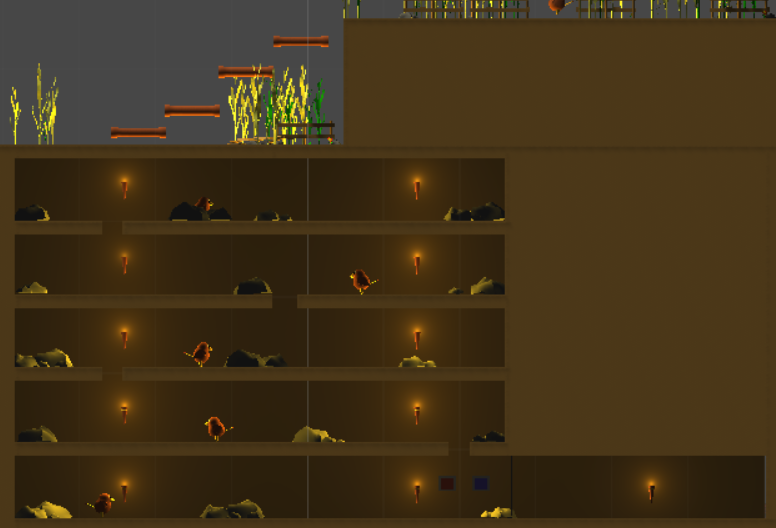
\includegraphics[scale=0.7]{Grafiken/Untergrund.png}
	\caption{Ansicht der Weggabelung zwischen dem nach oben f�hrenden Weg und dem Untergrund in 2D (f�r Spieler, die die Herausforderung meiden)}
	\label{grafik: untergrund}
\end{figure}

\subsubsection{Der Untergrund}

Auf seinem weiteren Weg gelangt der Spieler an die erste Weggabelung, welche in Abbildung \ref{grafik: untergrund} dargestellt wird. Der Weg nach oben ist hier der gew�nschte, w�hrend es sich bei dem Untergrund, der durch ein kleines Loch in der Erde betreten werden kann, um den unerw�nschten handelt.\\
Hier soll zun�chst mit Hilfe von auf die Spielereigenschaften abgestimmten Wegmerkmalen von dem unerw�nschten, unteren Weg abgelenkt werden. Dies geschieht f�r unaufmerksame Spieler, indem ein Stein, der jedoch vom Spieler zerst�rt werden kann, den Eingang blockiert, so dass diese nicht sofort auf ihn aufmerksam werden. Dahingegen besteht die Ablenkung f�r aufmerksame Spieler darin, dass die Baumst�mme zum oberen Weg gl�nzen, wodurch sie sich diesem zuwenden sollen.\\
Ist der dritte Baumstamm des oberen Weges einmal erreicht, st�rzt der Eingang zum Untergrund au�erdem vollst�ndig ein, so dass nicht mehr nachvollzogen werden kann, wohin er gef�hrt h�tte. Auf diese Art und Weise soll dem Spieler das Gef�hl vermittelt werden, dass ihm die Schuld daf�r zukommt, dass er nun diesen Weg nicht mehr erkunden kann, da er ihn zun�chst ignoriert hat.\\
F�r Spieler, die die Herausforderung suchen, gilt stets (auch f�r sp�tere Manipulationen), dass sich auf dem geplanten Weg mehr Gegner befinden als auf dem nicht vorgesehenen. Umgekehrtes z�hlt f�r Spieler, die Herausforderungen meiden. Bei dieser Manipulationsstrategie ist zu beachten, dass sie nicht vollst�ndig  auf den Abbildungen dargestellt werden kann, da die zus�tzlichen V�gel je nach Eigenschaft ein- oder ausgeblendet werden. So ist auf den Grafiken immer die Variante f�r Spieler zu sehen, die die Herausforderung meiden.\\
Dar�ber hinaus werden bei allen r�umlichen Manipulationen fortlaufend mehr Diamanten auf dem gew�nschten als auf dem nicht gew�nschten Weg platziert. Dabei wird nicht zwischen Sammlern und Nicht-Sammlern unterschieden, da nicht davon auszugehen ist, dass sich Nicht-Sammler von zu vielen Diamanten abschrecken lassen w�rden, aber Sammler sehr wohl von Wegen, die weniger Diamanten bereithalten als ein alternativer Pfad. �hnliches wurde f�r leichte Wege entschieden, so dass die nicht vorgesehenen Pfade stets schwieriger sind. In diesem Fall wird dies durch die sehr schmalen �berg�nge zwischen den Untergrundebenen erreicht. In der Platzierung der Diamanten zeigt sich au�erdem erneut die Manipulation des \textit{Anreizes durch die Beute}.

\subsubsection{Die Lava}

F�r den Fall, dass der Spieler sich dennoch daf�r entscheidet den Untergrund zu betreten, wurde eine weitere Manipulation eingebaut. So gelangt der Spieler am Ende des Weges an ein Gitter, neben dem sich zwei Schalter befinden. Auf diese Art und Weise soll suggeriert werden, dass hier ein weiterf�hrender Weg erreicht werden kann, indem das Gitter mit einem der Schalter ge�ffnet wird. Allerdings f�hren beide dazu, dass sofort t�dliche Lava aufsteigt, die den Spieler wieder an die Oberfl�che zwingt. Ist er hier angekommen, st�rzt der Eingang zum Untergrund ein. So soll erreicht werden, dass der Spieler sich selbst die Schuld daf�r gibt, dass er den falschen Schalter bet�tigt und somit die Falle ausgel�st hat, anstatt das Gitter zu �ffnen.\\
Diese Manipulation ist der Kategorie der \textit{Verschleierung des fehlenden alternativen Weges} (siehe Abschnitt \ref{subsec:ausgew�hlte strategien}) zuzuordnen.

\subsubsection{Ablenkung durch mehrere Wege}

In Abschnitt \ref{sec:dosierung von manipulationen} wurde bereits erl�utert, wie wichtig es ist, dass die Dosierung von Manipulationen nicht zu hoch wird, da sie sonst Gefahr laufen entdeckt zu werden. Aus diesem Grund wurde neben diesen Beeinflussungen auch versucht dem Spieler tats�chlich kleinere eigene Entscheidungen zu �berlassen, bei denen es sich jedoch letztendlich nur um kleine Abweichungen vom vorgesehenen Weg handelt (siehe Abschnitt \ref{subsec:ausgew�hlte strategien} \textit{Verschleierung des fehlenden alternativen Weges}). Genau dies wurde an der in Abbildung \ref{grafik: bruecken wege} gezeigten Stelle getan, an der der Spieler Br�cken erklimmen muss, die nur von unten durchl�ssig sind. Dabei sind die Wege so gestaltet, dass der Spieler beim Betreten des einen Weges den anderen nicht sehen kann, weil auf diese Art und Weise nicht offensichtlich wird, dass beide Wege schlie�lich zum selben Punkt f�hren. Da es au�erdem nicht m�glich ist von einem der beiden Wege den jeweils anderen zu erreichen oder wieder zur�ck zum Entscheidungspunkt zu gelangen, kann der Spieler diesen Verlauf auch nicht eindeutig nachvollziehen.

\begin{figure}[h]
	\centering
	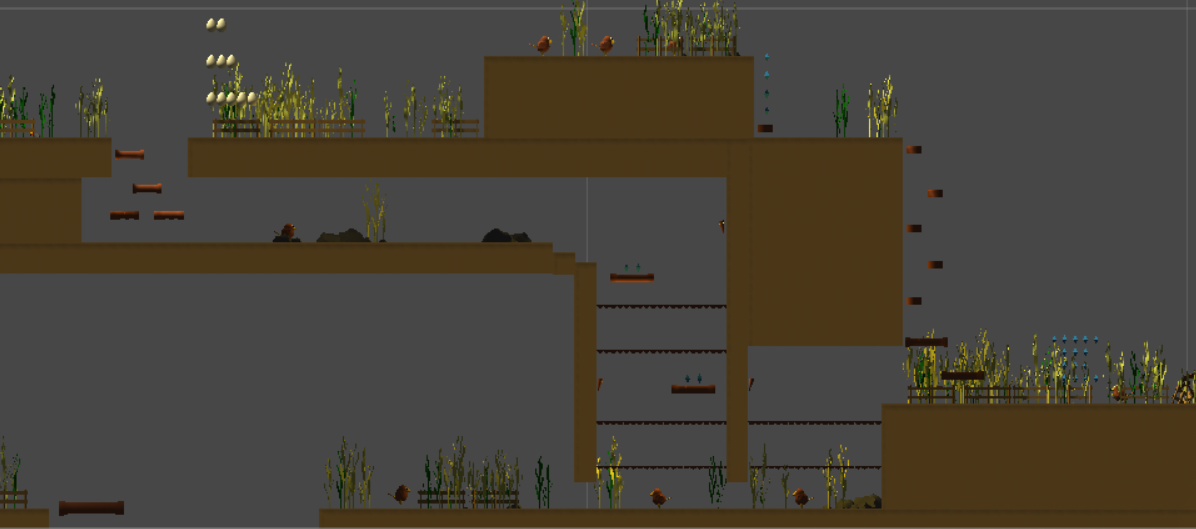
\includegraphics[scale=0.6]{Grafiken/Bruecken.png}
	\caption{2D-Darstellung der beiden m�glichen Wege �ber die Br�cken, die sich schlie�lich wieder treffen}
	\label{grafik: bruecken wege}
\end{figure}

\subsubsection{Das Versteck der V�gel}

Im weiteren Verlauf des Levels gelangt der Spieler durch einen Busch in das Versteck der V�gel, wo er einer erneuten Manipulation, die in Abbildung \ref{grafik: eingang versteck schr�ge} (a) gezeigt wird, gegen�bersteht. Hier soll er dazu gebracht werden nach rechts zu laufen. Zu diesem Zweck wird erneut das Prinzip verfolgt, dass sich auf dem richtigen Weg mehr Diamanten befinden, w�hrend der falsche unter anderem dadurch gekennzeichnet ist, dass er aufwendiger zu �berwinden ist. Auch das zuvor im Unterabschnitt \glqq Der Untergrund\grqq{} erkl�rte Vorgehen, dass je nach Auspr�gung der Herausforderungseigenschaft entweder mehr Gegner auf dem falschen oder dem richtigen Weg platziert sind, findet Verwendung. Der linke Weg ist au�erdem so gestaltet, dass sein Ende nicht abzusehen ist, um ungeduldige Spieler weiter von ihm abzulenken.\\
Die Hauptmanipulation besteht hier allerdings darin, dass von rechts eine Kiwano nach Hilfe ruft, was den Spieler auf den rechten, erw�nschten Weg aufmerksam machen soll. Diese Strategie geht auf das in Abschnitt \ref{subsec:ausgew�hlte strategien} beschriebene Konzept der \textit{Umgebungshinweise} zur�ck.

\begin{figure}[h]
	\centering
	\begin{minipage}[b]{0.55\linewidth}
		\centering
		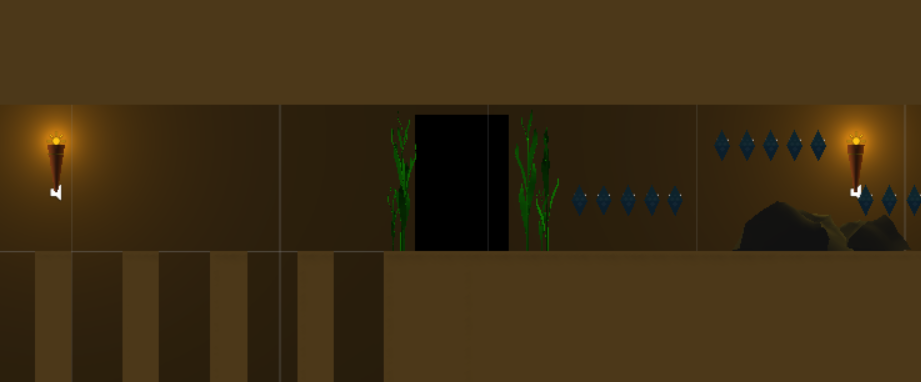
\includegraphics[width=\textwidth]{Grafiken/Eingang_Versteck.png}
		(a)
	\end{minipage}
	\begin{minipage}[b]{0.4\linewidth}
		\centering
		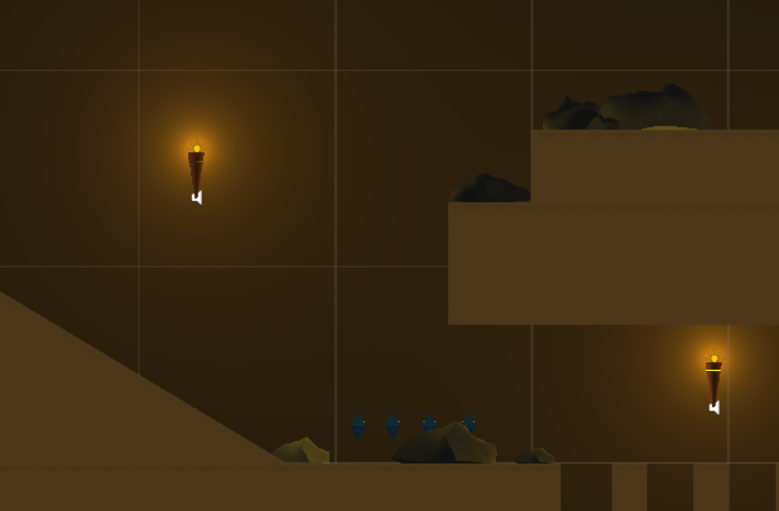
\includegraphics[width=\textwidth]{Grafiken/Schraege_in_Versteck.png}
		(b)
	\end{minipage}
	\caption{2D-Ansicht des Eingangs im Versteck der V�gel f�r Herausforderungen meidende Spieler (a) und der Schr�ge vor der Sackgasse (b)}
	\label{grafik: eingang versteck schr�ge}
\end{figure}

\subsubsection{Die Schr�ge}

Bei dieser Strategie handelt es sich um eine Absicherung zur vorhergehenden Manipulation. So gelangen Spieler, die trotz aller Ablenkung den linken Weg w�hlen, an eine Schr�ge, �ber der sich eine Plattform befindet (siehe Abbildung \ref{grafik: eingang versteck schr�ge} (b)). An dieser Stelle soll ihm suggeriert werden, dass es einen weiteren m�glichen Weg gibt, welcher jedoch in Wahrheit in einer Sackgasse endet, die der Spieler von hier aus jedoch nicht sehen kann. So wird er wahrscheinlich versuchen die Plattform �ber die Schr�ge zu erreichen, allerdings ist diese mit einer rutschigen Schicht �berzogen, durch die der Sprung stets ein wenig zu kurz ger�t, so dass das Plateau zwar unerreichbar bleibt, aber die Hoffnung des Spielers, dieses k�nne irgendwie noch bezwungen werden, nie ganz erlischt, wodurch er die Schuld erneut bei sich sucht und nicht beim Spiel. Um diesen Eindruck zu verst�rken sind auch auf der Plattform Dekorationsgegenst�nde platziert. Somit handelt es sich erneut um die \textit{Verschleierung des Fehlens eines alternativen Weges}.

\subsubsection{Der t�dliche Vogelschwarm}

Die n�chste Manipulationsstrategie bezieht sich auf das Konzept des \textit{Zeitdrucks} (siehe Abschnitt \ref{subsec:ausgew�hlte strategien}). So erreicht der Spieler bald ein nach oben f�hrenden Vogelhorst mit Nestern, die von V�geln bewacht werden, und von denen das obere auch die gesuchte Kurbel enth�lt. Beim Finden dieser ist die Decke des Verstecks noch nicht zu sehen, so dass der Spieler denken k�nnte, dass er hier eventuell weiterkommt. Doch bevor er genauer dar�ber nachdenken kann, naht ein riesiger, sofort t�dlicher Vogelschwarm von oben heran, so dass der Spieler, �hnlich wie bei \glqq Die Lava\grqq{}, gezwungen wird schnell das Versteck �ber den Ausgang zu verlassen. Auf diese Art und Weise soll erneut sichergestellt werden, dass er nicht dem Spiel, sondern sich selbst die Schuld daf�r gibt, dass er vor dem Aufheben der Kurbel nicht weiter das Versteck erkundete, indem er beispielsweise den linken Weg am Eingang genommen oder die nach oben offene Decke des Horstes untersucht h�tte. Somit handelt es sich auch um eine \textit{Verschleierung des Fehlens eines alternativen Weges}. Au�erdem wird davon ausgegangen, dass der Spieler nicht darauf kommt vielleicht doch noch den linken Weg am Eingang zu nehmen, da er in einem geschlossenen Versteck damit rechnen muss sonst irgendwann von dem Vogelschwarm in die Ecke gedr�ngt zu werden.

\subsubsection{Higgins}

Bei Higgins, einem von Black Sparrows Handlangern, handelt es sich um den Endboss des Levels. Er muss besiegt werden, bevor der Spieler von hier aus in den dunklen Wald (Abschnitt \ref{subsec: der dunkle wald}) gelangen kann.

\subsection{Level 3.1: Der dunkle Wald}
\label{subsec: der dunkle wald}

In diesem Level angekommen, muss der Spieler nur noch den dunklen Wald vor Black Sparrows Nest durchqueren, um schlie�lich zu ihm zu gelangen und Cherry retten zu k�nnen. Auch hier findet er einen Wegweiser. Dieser dient erneut dem Zweck, dass der Spieler sich gegebenenfalls noch umentscheiden und sich bei den anderen Fr�chten Verst�rkung holen kann, falls er dies noch nicht getan hat, was  ebenfalls wieder dem Zweck dient ein Gef�hl der Entscheidungsfreiheit zu schaffen.

\subsubsection{Die leuchtende H�hle}

Kurze Zeit nachdem der Spieler das Level betreten hat, gelangt er an die in Abbildung \ref{grafik: leuchtende h�hle} gezeigte Stelle. Hier wird eine andere Art von \textit{Umgebungshinweis} verwendet, indem dieses Mal mit Hilfe eines Leuchtens, welches aus der H�hle dringt, versucht wird auf den gew�nschten Weg aufmerksam zu machen.\\
Dar�ber hinaus werden auch hier wieder die auf die Spielereigenschaften abgestimmten �nderungen vorgenommen, so dass Herausforderungen meidende Spieler auf dem oberen Weg mehr Feinde zu sehen bekommen, w�hrend es f�r Herausforderungen suchende andersherum ist.\\
Dieses Mal wird auch versucht unaufmerksame Spieler damit zu k�dern, dass die nach oben f�hrenden Eier gl�nzen, so dass sie diese m�glicherweise gedankenlos zerst�ren und es ihnen so nicht mehr m�glich ist den unerw�nschten, oberen Weg zu erreichen. Gleichzeitig ist der Weg �ber die Eier so angelegt, dass er einiges Geschick verlangt, um ihn erfolgreich zu erklimmen und abermals befinden sich auf dem unteren Weg mehr Diamanten. Diese sind au�erdem so platziert, dass ungeschickte Spieler beim Einsammeln den Weg nach oben zerbrechen und somit wieder die Schuld f�r das Nicht-Erreichen dieses Weges bei sich selbst suchen.

\begin{figure}[h]
	\centering
	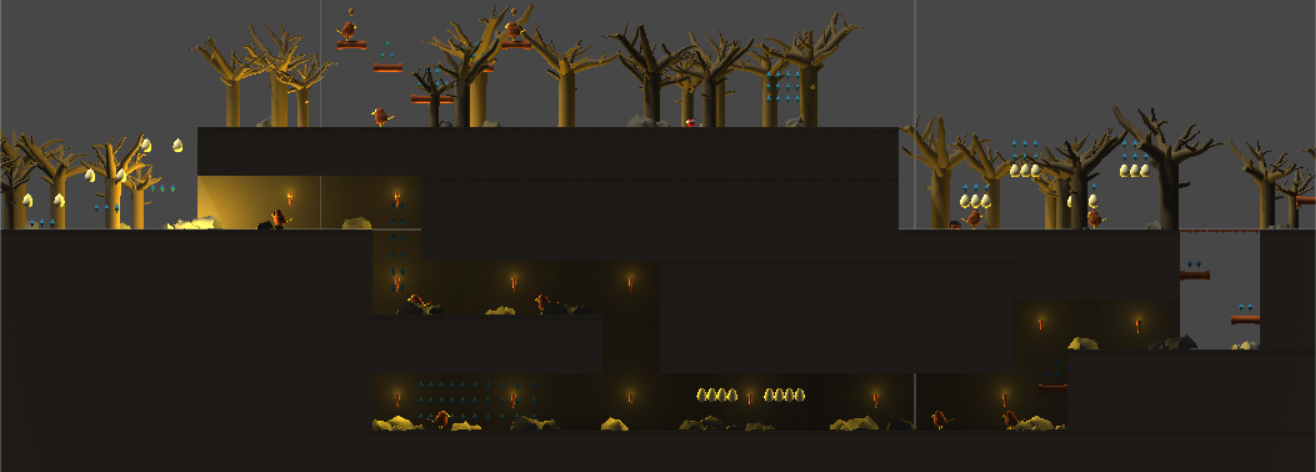
\includegraphics[scale=0.6]{Grafiken/Hoehle.png}
	\caption{2D-Ansicht der Weggabelung vor der H�hle sowie der weiteren Wegverl�ufe f�r einen Herausforderungen meidenden Spieler}
	\label{grafik: leuchtende h�hle}
\end{figure}

\subsubsection{Eine weitere Ablenkung}

An dieser Stelle (ebenfalls Abbildung \ref{grafik: leuchtende h�hle}) existiert eine weitere, die vorherige Manipulation absichernde \textit{Ablenkung des Spielers von dem Fehlen eines alternativen Weges}. So f�hrt auch der Weg nach oben letztendlich wieder auf den gew�nschten Weg zur�ck, wobei hier erneut darauf geachtet wurde, dass der Spieler nicht direkt sehen und nachvollziehen kann, ob beide Pfade zum selben Ziel f�hren. Dies wird einerseits dadurch verhindert, dass der Spieler die nur von unten durchl�ssige Br�cke �ber dem H�hlenweg nicht erneut durchqueren kann, und andererseits dadurch, dass die Erh�hung, auf der der obere Weg liegt, nicht von rechts erklommen werden kann, hat der Spieler sie einmal verlassen.\\
Dar�ber hinaus wird der kommende Questgeber je nach Entscheidung des Spielers auf dem oberen oder unteren Weg platziert, um ihn im Falle des oberen Weges nicht merken zu lassen, dass dieser unwichtig war.

\subsubsection{Manfreds verlorene Sachen}

Diese Manipulation geht auf den in Abschnitt \ref{subsec:ausgew�hlte strategien} beschriebenen Entwurf der \textit{Motivation zu Aufgaben durch Anfangserfolge} zur�ck. Daher wird sie bereits am Anfang des Levels eingeleitet, als der Spieler auf einen Hut st��t, den er aufheben kann. Tut er dies, fragt sich Antonio dabei laut, wem dieser wohl geh�rt, um den Spieler neugierig zu machen. Kurz darauf trifft er auf Manfred, eine verletzte Kirsche, die ihn bittet f�r ihn seine, von den V�geln gestohlenen, Sachen zur�ckzubringen. Auf diese Art und Weise soll das bereits im entsprechenden Unterabschnitt beschriebene Prinzip verfolgt und der Spieler animiert werden die fehlenden Sachen auch noch finden zu wollen.\\
Des Weiteren gibt es erneut eine Belohnung bei der Erledigung der Aufgabe, was jedoch nur eine weniger gewichtige, sekund�re Manipulation darstellen soll und eher ein Nebeneffekt ist, da Belohnungen im Allgemeinen �blich f�r das Erf�llen von Quests sind.

\subsubsection{Die Verfolgung}

Hier wird erneut das Mittel des \textit{Zeitdrucks} angewendet. So ger�t der Spieler in ein Gespr�ch zwischen zwei V�geln, in dem suggeriert wird, dass diese gerade auf dem Weg zu Black Sparrows Nest sind, womit sich ihm die Gelegenheit bietet ihnen unauff�llig zu folgen, um sich dann hinter ihrem R�cken in das Nest hineinzuschleichen. Doch da die beiden V�gel sich schnell bewegen, muss er sich beeilen, wodurch er dazu gedr�ngt werden soll die von ihrem Weg abweichenden Pfade zu ignorieren, um sie nicht zu verlieren. Um dieses Gef�hl zu verst�rken, wird der Spieler stets wieder an den Anfang des Dialogs zwischen den beiden V�geln versetzt, solle er ihnen zu nahe kommen und entdeckt werden oder sie aus den Augen verlieren.\\
Um diesen vermeintlich alternativen Wege au�erdem eine gewisse Attraktivit�t zu verleihen, werden auch auf diesen Gegenst�nde platziert, da sonst davon auszugehen ist, dass der Spieler sie auch ohne den Zeitdruck nicht als interessant genug wahrgenommen h�tte.

\subsection{Level 3.2: Black Sparrows Nest}
\label{subsec: black sparrow nest}

Black Sparrows Nest stellt das Endlevel des Spiels dar, in dem Billy Black Sparrow und Antonio besiegen muss, um schlie�lich Cherry retten zu k�nnen. Im Folgenden sollen die Manipulationen, die dabei eingesetzt werden, erl�utert werden. Wichtig ist auch hier wieder der am Anfang des Levels befindliche Wegweiser, wie sich im Unterabschnitt zum Kampf gegen Black Sparrow noch zeigen wird.

\subsubsection{Antonios kleiner Bruder}

An dieser Stelle soll die Manipulation durch die \textit{Anfrage von kameradschaftlichen Charakteren} getestet werden. So erz�hlt Antonio auf dem Weg zu Black Sparrow pl�tzlich davon, dass er noch einen kleinen Bruder habe, der ebenfalls von den V�geln entf�hrt worden sei, woraufhin er Billy bittet diesen f�r ihn zu suchen. Hier kann der Spieler zwar erneut in einem Dialog mit Antonio diskutieren auf welche Art und Weise oder ob sie diesen suchen wollen, aber letztendlich l�uft das Gespr�ch darauf hinaus, dass die beiden sich trennen, auch wenn der Spieler die Suche nach dem Bruder ablehnen sollte. Das eigentliche Ziel ist jedoch, dass der Spieler diese Anfrage annimmt, da er anhand von Antonios Verhalten, welches bereits in Abschnitt \ref{subsec:ausgew�hlte strategien} unter der entsprechenden Manipulation erl�utert wurde, eine gewisse Sympathie f�r ihn empfinden soll.

\subsubsection{Die einst�rzende Br�cke}

Um diesen \glqq harten\grqq{} Verlauf bei dem Gespr�ch zwischen Antonio und Billy ein wenig abzuschw�chen, kann der Spieler dem nach oben weglaufenden Antonio folgen. Er wird jedoch dadurch aufgehalten, dass dieser, auf einem Plateau angekommen, �ber eine Br�cke l�uft, die direkt hinter ihm zusammenst�rzt, so dass der Spieler die noch nicht eingest�rzten Segmente gerade so nicht erreicht, wodurch er erneut sich die Schuld geben k�nnte, da er Antonio vielleicht h�tte folgen k�nnen, w�re er ein wenig schneller oder geschickter gewesen. Das Plateau befindet sich au�erdem so weit oben, dass der Spieler abermals nicht sehen kann, dass die Br�cke eigentlich in eine Sackgasse f�hrt. Damit handelt es sich hier erneut um ein \textit{Verschleiern des Fehlens eines alternativen Weges}.

\subsubsection{Der Kampf gegen Black Sparrow}

Diese Szene geh�rt zu einer langfristigen Ablenkung davon, dass der Spieler eben doch nicht so frei entscheiden kann, was im Spiel geschieht (\textit{Verschleierung des Fehlens eines alternativen Weges}). So soll versucht werden den Spieler sp�testens im Kampf gegen Black Sparrow darauf zu bringen, dass es alleine zu aufwendig und langwierig ist diesen zu besiegen. Dadurch gilt es zu erreichen, dass er sich schlie�lich doch Hilfe bei den Kiwanos holt.\\
Die Schwierigkeit beim Kampf gegen Black Sparrow wird hier einerseits dadurch erreicht, dass sich der in Level 2.1 erw�hnte Higgins zu ihm gesellt, da dieser noch nicht vom Spieler im Dorf der Kiwanos besiegt wurde, und andererseits dadurch, dass das Schild tats�chlich einen wichtigen Schutz beim Kampf gegen den schweren Endboss bietet. Wesentlich ist bei dieser Strategie ebenfalls, dass der Spieler keinesfalls denken soll, dass Black Sparrow ohne die Hilfe unbesiegbar w�re, da er sich sonst zu sehr beeinflusst f�hlen k�nnte.\\
Das Zur�ckkehren in das Dorf der Kiwanos ist wieder �ber einen Wegweiser m�glich.

\subsubsection{Antonios Verrat}

Das Finale des Spiels findet statt, als Billy nach dem Kampf gegen Black Sparrow auf Antonio trifft, welcher Cherry bereits gefunden hat und sie nun f�r sich beanspruchen will, da er seit jeher in sie verliebt ist und immer eifers�chtig auf sie und Billy war. Aufgrund dieses Verrats soll der Spieler trotz seiner eigentlichen Sympathie zu Antonio dazu animiert werden, sich im Dialog mit ihm daf�r zu entscheiden ihn anzugreifen (siehe Abschnitt \ref{subsec:ausgew�hlte strategien} \textit{Nutzung des Gerechte-Welt-Glaubens}). Um dem Spieler auch hier noch eine gewisse \glqq Schein-Freiheit\grqq{} zu lassen, kann er allerdings auch Cherry entscheiden lassen oder versuchen Antonio nicht anzugreifen, was jedoch ebenfalls fr�her oder sp�ter dazu f�hrt, dass Antonio seinerseits den Spieler angreift.

\section{Zusammenfassung}
\label{sec:zusammenfassung konzeption}

In diesem Kapitel sind zun�chst, basierend auf den Grundlagen (siehe Abschnitt \ref{chap:grundlagen manipulation}), die allgemeinen Anforderungen und Einschr�nkungen, die bei der Auswahl geeigneter Manipulationen zu beachten waren, erl�utert worden. So wurde festgestellt, dass m�glichst positive Manipulationsstrategien, die f�r weniger Frust beim Spieler sorgen, zu verwenden sind sowie dass diese auch den Kriterien der Unauff�lligkeit und der Anwendbarkeit auf einen m�glichst weiten Personenkreis gen�gen m�ssen. Au�erdem war es notwendig aufgrund fehlender Ressourcen (wie z.B. der Entwicklungszeit) auf �ber eine l�ngere Zeitspanne aufzubauende sowie durch Emotionen bedingte Manipulationen zu verzichten. �hnliches gilt f�r die Verwendung der Theorie des sozialen Vergleichs und von Questtageb�chern, wobei Letzteres vor allem nicht zum Genre des Jump and Runs passte.\\
Anschlie�end wurden die Ergebnisse des Auswahlverfahrens pr�sentiert. Diese umfassten neben den Armes-Schwein-Spielen und der Nutzung des Gerechte-Welt-Glaubens ebenfalls die Verschleierung fehlender alternativer Wege, Umgebungshinweise sowie Anfragen von kameradschaftlichen Charakteren. Des Weiteren wurde auch das Prinzip des Anreizes durch die Beute und des Zeitdrucks als sinnvoll erachtet.\\
Dar�ber hinaus ist auch die Auswahl der Spielereigenschaften getroffen worden. Diese sollen dazu dienen die Manipulationen durch eine Abstimmung auf die Pers�nlichkeit des Spielers zu unterst�tzen. So schien es angemessen den Spieler sowohl nach seiner Sammelleidenschaft, seinem Ehrgeiz sowie seiner Geduld und Aufmerksamkeit zu beurteilen als auch darauf zu achten ob er Herausforderungen sucht und inwiefern er in der Lage ist Mitleid zu empfinden. Au�erdem spielte auch der Drang des Spielers nach Autonomie eine Rolle.\\
Den Abschluss bildete schlie�lich die auf den vorherigen Ergebnissen aufbauende Konzeption der Level des Prototypen.

%................................................................
					
	% Implementierung einbinden
	%#####################################################################################################################
% Datei	: Grundlagen.tex
% Autor	: Implementierung Worms
%#####################################################################################################################
\chapter{Prototypische Umsetzung}
\begin{itemize}
	\item Wieso die prototypische Umsetzung?
	\item Ziel der prototypischen Umsetzung
	\item �bersicht mit kurzer Erl�uterung der Implementierten Strukturen
\end{itemize}

\subsubsection*{Entwicklungsumgebung}
W�hrend der Anfangsphase der prototypischen Umsetzung m�ssen zun�chst die technischen Grundlagen und die eventuell 
vorhandenen Hilfsmittel abgesteckt und benannt werden. Die folgenden Varianten wurden auf Machbarkeit, Effizienz 
und Tauglichkeit hin f�r \textit{Billy's Payback} analysiert:
\begin{itemize}[itemsep=0pt] 
	\item ???: S�mtlich anfallende Aufgabenbereiche m�ssen von Grund auf entwickelt und implementiert werden. Die Variante bietet
	neben einem sehr hohen Aufwand gleichzeitig eine gute Flexibilit�t in Bezug auf die Gestaltungsfreiheiten an.
	\item Hybridsystem: Zu verallgemeinernde und wiederkehrende Strukturen werden mittels externen Fremdbibliotheken vereinfacht
	in Form von Bauteilen dem Anwender bereitgestellt. Das Zusammenspiel der unterschiedlichen Komponenten muss nach wie vor
	selbstst�ndig erarbeitet werden. Beispiele f�r Bibliotheken sind Grafik-, Audio- sowie Physikbibliotheken.
	\item Vollst�ndiger Toolchain: Das Management f�r das Zusammenspiel der einzelnen Komponenten wird (komplett) von einer
	sogenannten \textit{Game--Engine} bereitgestellt, sodass die Konzentration auf die alleinige Spielentwicklung und --Gestaltung
	gerichtet werden kann.
\end{itemize}
Basierend auf den zeitlichen Restriktionen f�r das Projekt ist die Variante mit dem vollst�ndigen Toolchain zum Einsatz gekommen.
Anl�sslich der hohen Anzahl von existierenden \textit{Game--Engines} wurde der nachstehende Anforderungskatalog aufgestellt
und f�r die Entscheidungsfindung zu Hilfe genommen:
\begin{itemize}[itemsep=0pt] 
	\item Kostenlose Version f�r Entwicklungen und Ver�ffentlichungen von Inhalten.
	\item Komprimierte und innovative Einarbeitung in grundlegenden Thematiken der \textit{Engine} m�glich.
	\item Realisierung von eigenen Scripten in einer bekannten Sprache ausf�hrbar (keine hauseigene Scriptsprache).
	\item Zuschnitt auf ein breites Spektrum von Genres (keine einschr�nkenden oder zeitaufwendigen Vorgaben).
\end{itemize}
Nach einer eingehenden Analyse vorhandener \textit{Game--Engines} hinsichtlich des Anforderungskatalogs, wie zum
Beispiel die \textit{CryEngine}~\cite{CryEngine} und die \textit{UnrealEngine}~\cite{UnrealEngine}, ist die
\textit{Unity--Engine}~\cite{Unity} f�r die prototypische Umsetzung ausgew�hlt worden.

\subsubsection*{Projektversionierung}
Bei gr��eren Softwareprojekten bietet sich die M�glichkeit an, die eingehenden �nderungen an der Struktur des Codes in
regelm��igen Abst�nden zu protokollieren. Ein weiteres, nicht zu untersch�tzendes Features stellt die Archivierung der durch die beteiligten
Entwickler eingetragenen Ver�nderungen dar, sodass ein vorheriger Stand der Arbeit unter bestimmten Voraussetzungen wiederherstellbar
ist.
\\
F�r die sogenannte \textit{Versionsverwaltung} existieren unterschiedliche Konzepte und Realisierungsans�tze, zu denen sowohl
\textit{Subversion (SVN)} als auch \textit{GIT} z�hlen. F�r den prototypischen Anteil der wissenschaftlichen Arbeit
diente \textit{GIT} aus den nachstehenden Gr�nden als Versionierungswerkzeug:
\begin{itemize}[itemsep=0pt] 
	\item Im Gegensatz zu \textit{SVN} stellt \textit{GIT} eine verteilte Versionierungsplattform dar. Hierbei werden die Daten
	nicht ausschlie�lich auf dem zentralen Verwaltungsserver archiviert, sondern jeder beteiligte Entwicklungscomputer enth�lt
	eine lokale Kopie des \textit{Repositories}.
	
	\item Die lokal gespeicherten \textit{Repositories} bieten die M�glichkeit bereits kleine lokale �nderungen zu
	protokollieren, ohne dass diese unmittelbar sichtbar f�r die anderen Entwickler werden. Die Arbeit an dem Projekt ohne eine
	bestehenden Internetverbindung wird ebenfalls durch die eigenst�ndigen \textit{Repositories} beg�nstigt.
\end{itemize}

\subsubsection*{Implementierte Strukturen}
Code:
\begin{itemize}
	\item Die wichtigsten Implementierung (bis auf 2 Partikelsysteme alles selber gemacht)
	\item Aufteilung in die unterschiedlichen Gamestates (Prototyp -> nur das notwendigste ausgef�llt)
	\item Ablaufsteuerung innerhalb des Spiel �ber eine FSM gel�st (kurze Erl�uterung, evtl. kleines Diagramm)
	\item Dialogsystem mit Integration in der FSM (flexibles Dateiformat "entwicklet" -> kurz Vorz�ge erl�utern)
	\item Aktoren (kurze Erl�uterung �ber generelle Funktionsweise)
	\item Screenshots im Anhang
\end{itemize}

%....................................................................................................................
% Hier die Sektionen f�r die Umsetzung
%....................................................................................................................
	
	% Evaluierung einbinden			
	%#####################################################################################################################
% Datei	: Evaluierung.tex
% Autor	: Byron Worms
%#####################################################################################################################
\chapter{Evaluierung}
\label{chap:evaluierung}

In diesem Kapitel soll zun�chst besprochen werden, wie gut die Auswertung der Eigenschaftenanalyse funktioniert hat. Die Probanden sollten gem�� den Eigenschaften Sammler, Geduld, Ehrgeiz, Herausforderung, Mitleid, Autonomie und Aufmerksamkeit beurteilt werden. Anschlie�end erfolgt die Auswertung des Interviews mit den Probanden, welche auch gezielte Fragen zu den einzelnen Manipulationen enthalten. Dabei werden positive Aspekte, Gr�nde und auch Verbesserungsm�glichkeiten vorgestellt. Abschlie�end wird auf die allgemeinen Fragen zum Spiel eingegangen und die Erfolgskriterien bewertet, sodass ein Fazit getroffen werden kann, wie erfolgreich insgesamt die verwendeten Manipulationen waren.

%................................................................
\section{Auswertung Eigenschaftenanalyse}
\label{sec:auswertung eigenschaftenanalyse}

\subsection{Fehlerquellen in der Umsetzung}
\label{subsec:fehlerquellen in der umsetzung}

Eine gro�e Fehlerquelle war die ung�nstige Platzierung der Trigger, die f�r die Analyse der Eigenschaften dienen sollten. Dies hatte zur Folge, dass manche Probanden falsch bewertet und die nachfolgenden Level nicht entsprechend korrekt aufgebaut wurden. Problematisch dabei war die Annahme, dass der Spieler immer linear weiter laufen und nicht vor- und zur�ckspringen bzw. beide Wege abdecken soll. So kann gleich bei dem ersten Diamanten im Spiel passieren, dass der Spieler zun�chst dar�ber springt und als Nicht-Sammler klassifiziert wird. Kehrt der Spieler dann aber zur�ck und sammelt den Diamanten ein, ist er offensichtlich doch ein Sammler. Bei der kleinen Kirsche, bei der der Spieler eine Aufgabe annehmen konnte, waren vier V�gel auf einem Plateau zu besiegen. Der Trigger wurde aber erst weiter hinten bei den Eltern der Kirsche gesetzt. Besiegt der Spieler die V�gel und geht nicht weiter zu den Eltern vor, l�st er den Trigger ggf. nicht aus. Eine weitere Problemstelle war der bewegliche Baumstamm unter den vielen kleinen Baumst�mmen. W�hlt der Spieler den oberen, schwierigeren Weg und f�llt dann runter auf dem Baumstamm, der ihn auf die andere Seite bringt, wird nicht das Nehmen des oberen, sondern das des unteren Weges gez�hlt. Die letzte Fehlplatzierung befand sich bei dem Pfeilschild, wo unter anderem die Geduld des Spielers getestet werden sollte, indem unter dem Baumstamm langsam V�gel hervorkamen. Der Trigger befand sich am Ende des unteren Baumstamms. Die meisten Spieler, die warteten, haben nur die V�gel besiegt und sich dann f�r den oberen Weg entschieden und haben so den vorgesehenen Trigger nicht erreicht. \\

Eine weitere Fehlerquelle ist die fehlende Sichtbarkeit einiger Punkte, die zur Verzerrung der Bewertung f�hrten. Dazu z�hlen zum Beispiel die Diamanten, die sich vor der gro�en Schlucht in einer kleinen Einbuchtung befinden. Auch die Kuhle mit den vielen V�geln wurde nicht als solches erkannt, sondern als eine Art Schlucht, �ber die man springen muss, um nicht zu sterben. Oftmals war es den Probanden nicht klar, dass der bewegliche Baumstamm auch zum Ziel f�hrt. Dieser war zun�chst mit dem Gedanken an 2D-Jump-and-Runs entworfen worden, wo der Querschnitt des Bodens ebenfalls sichtbar ist, sodass man den Baumstamm und das zu erreichende Ziel auch gleich erkennt. Am Ende des Levels ist die zu rettende Kirsche nicht mehr erreichbar, wenn der Spieler schon alle Eier zerst�rt hat, sodass auch bei Mitleid des Spielers diese Eigenschaft nicht mehr erfasst werden konnte. Auch die Hilfeschreie dieser Kirsche wurden von den Probanden eher als witzig und nicht als mitleiderregend aufgefasst. Daraus und dass der Schrei in manchen F�llen schlecht wahrnehmbar war, l�sst sich schlie�en, dass dies nicht der richtige Anreiz war, um Mitleid erzeugen zu k�nnen.

\subsection{Verbesserungsm�glichkeiten}
\label{subsec:verbesserungsm�glichkeiten}

Eine wichtige technische Verbesserung w�re, dass das Triggersystem adaptiv arbeiten muss. Es muss auch F�lle abdecken, in denen der Spieler r�ckw�rts l�uft oder beide Wege nimmt. Dies f�hrt allerdings auch zu mehr Komplexit�t.

\subsection{Folgen}
\label{subsec:folgen}

\subsubsection{Sammler}

Als Folge wurde das Sammeln meist falsch bewertet. Die meisten Probanden sammelten viel bis sehr viel, bekamen aber negative Bewertungen auf die Eigenschaft Sammeln. Positiv zu erw�hnen ist, dass die Spieler tats�chlich bem�ht waren, die Diamanten zu sammeln. Diese boten also einen entsprechenden Anreiz. Manche Probanden haben allerdings nicht mitbekommen, dass sie dadurch mehr Leben bekommen, haben aber trotzdem gesammelt. Der zu schnelle Text k�nnte daf�r ein Grund sein. Weitere Gr�nde f�r die falsche Auswertung der Sammel-Eigenschaft liegen auch an dem bereits schon angesprochenen ersten Diamanten, der nachtr�glich noch eingesammelt werden konnte, sowie an den Diamanten, die sich in der Schlucht befanden, aber von den Probanden nicht gesehen wurden. Diese Stellen zu verbessern, w�rde eine korrektere Auswertung nach sich ziehen. Noch besser w�re aber die Analyse mittels eines Schwellenwertes, bei dem die Anzahl der gesammelten Diamanten mit der Anzahl der im Spiel befindlichen Diamanten verglichen wird. So ist die Sammeleigenschaft nicht nur an den Triggern festgemacht.

\subsubsection{Geduld}

Die gr��te Abweichung in der Analyse betraf die Eigenschaft Geduld. Bei einigen Probanden stimmte die Analyse mit dem Fragebogen �berein. Bei anderen ergab sie Ungeduld, obwohl sich die Probanden selbst als geduldig eingestuft hatten. Hierbei ist zu erw�hnen, dass die Einsch�tzung der Geduld im Fragebogen sehr subjektiv erfolgte und es nicht sicher ist, ob sich der Spieler richtig einsch�tzen konnte. Als weiterer Grund fehlte ein zus�tzlicher Anreiz an entsprechenden Stellen (z.B. durch Diamanten), um auch wirklich geduldig sein zu m�ssen. Der von uns gew�hlte Ansatz, dass der geduldigere Weg angenehmer ist, da der andere Weg schwieriger oder durch V�gel blockiert ist, funktioniert nur, wenn der Spieler Feinde und schwere Wege scheut. Auch der bereits oben erw�hnte falsch gesetzte Trigger bei dem Warten auf die V�gel bzw. das falsche Deuten des sich bewegenden Baumstammes sind m�gliche Gr�nde der Fehlanalyse. Verbesserungen k�nnten einerseits durch besseres Setzen der Trigger und das Geben von mehr Anreizen f�r die Wahl des geduldigen Weges erzielt werden. 

\subsubsection{Ehrgeiz}

Eher geringe bis gar keine Abweichungen gab es bei der Eigenschaft, ob der Spieler den schweren Weg eher nimmt als den leichten. Dies f�hrt zu der Schlussfolgerung, dass der schwere Weg am Anfang auch tats�chlich als solcher wahrgenommen wurde. Kaum ein Proband hat ihn gew�hlt. Wenn doch, dann wegen der sich dort befindlichen Diamanten oder der Proband sah diese Strecke als Herausforderung an und w�hlte sie deshalb, was auch so vorgesehen war. F�r die geringen Abweichungen sei wieder auf das bereits erw�hnte Herunterfallen vom schweren Weg auf den sich darunter bewegenden Baumstammes verwiesen. Auch ist die Wahrnehmung, ob ein Weg schwer oder leicht ist, abh�ngig vom Spieler und k�nnte so die Abweichungen im Fragebogen erkl�ren.

\subsubsection{Herausforderung}  

Auch bei der Eigenschaft der Herausforderung gab es meist nur geringe Abweichungen bei der Analyse. Die Analyse hat also diesbez�glich allgemein gut geklappt. Es gab nur einen Ausrei�er, der bei der Anzahl an Probanden vernachl�ssigbar ist. Positiv war hierbei, dass die Stellen bei der kleinen Kirsche und �ber dem matschigen Weg gut umgesetzt wurden. Der Spieler hatte bei der Aufgabe der kleinen Kirsche jederzeit die Wahl, aus Angst vor der Herausforderung auch abbrechen zu k�nnen. Der �berwiegende Teil der Spieler hat sich als mehr Herausforderung suchend empfunden (im Fragebogen) als dies von der Analyse bewertet wurde. Ein Grund ist einmal die Kuhle mit vielen Feinden drin, die als solche nicht erkannt wurde. Ein weiterer Grund ist das lange Warten auf die V�gel und die darauf folgende Wahl, trotzdem oben lang zu gehen, sodass der richtige Trigger nicht ausgel�st wurde. Verbesserungsm�glichkeiten sind somit das Beheben des Triggerproblems, sowie die Verbesserung der Sichtbarkeit der Kuhle.  

\subsubsection{Mitleid}

Bei der Mitleids-Eigenschaft gab es einige Abweichungen bei der Analyse, sowohl zu mehr als auch zu weniger Mitleid. Positiv hervorzuheben ist, dass erreicht werden konnte, dass ein Proband tats�chlich Mitleid mit der kleinen Kirsche hatte. Einige Gr�nde f�r die Abweichungen wurden bereits angesprochen. Dazu z�hlen der Weg zur Kirsche, der durch zerst�rte Eier unm�glich wurde, der nicht als Hilferuf wahrgenommene Schrei und der sich erst bei den Eltern befindliche Trigger. Alle drei Situationen sind Gr�nde daf�r, dass jemand als weniger mitleidig eingestuft wurde, als er eigentlich ist. Wie mitleidig sich der jeweilige Spieler selbst einstuft ist zudem wieder sehr subjektiv. M�glicherweise wollten die m�nnlichen Probanden ihr Mitleid nicht im Fragebogen zugeben. Auch ist oft die eigene Erfahrung ausschlaggebend, ob sich eine Person in die jeweilig Situation hineinversetzen kann (z.B. wie die Kirsche selbst Eltern verloren, etc.). Dies k�nnen sowohl Gr�nde f�r mehr als auch f�r weniger analysiertes Mitleid sein. Generell ist es schwierig, sich mit derart prototypischen und abstrakten Charakteren zu identifizieren. Es gibt einige Verbesserungsm�glichkeiten, die in diesem Fall getroffen werden k�nnen. Ein realistischerer Sound f�r den Schrei der Kirsche k�nnte beim Probanden mehr Mitleid erzeugen. Dies war f�r den Prototypen schwierig, da kostenlose Sounds nur schwer zu bekommen sind. Und auch das Einsprechen eines solchen ber�hrenden Schreis erfordert ebenfalls Geschick, welches nicht jeder besitzt. Als weiterer Punkt kann die Kombination mit den Eiern verbessert bzw. vermieden werden. Da der Spieler vorab lernt, die Eier zu zerst�ren, ist es nicht zielf�hrend, diese f�r den Weg zur Kirsche zu verwenden. Wichtiger w�re gewesen, beide Eigenschaften einzeln zu testen (einmal Mitleid f�r die Kirsche und einmal Aufmerksamkeit durch die gl�nzenden Eier). Allerdings bleibt zu sagen, dass es eher schwer ist, subjektive und individuelle Abweichungen bei der Bewertung und Analyse des Mitleids zu umgehen. Es kann maximal versucht werden, die Charaktere realistischer zu gestalten und �ber eine l�ngere Zeit eine Beziehung zu ihnen aufzubauen, damit der Spieler eine parasoziale Beziehung eingeht. Dies ist jedoch im Rahmen eines kurzen Prototypen nicht m�glich. Auch m�sste die Story bunter und vielf�ltiger ausgebaut werden, damit sich der Spieler besser hineinf�hlen kann, was wiederum erst in fertigen Spielen wirklich m�glich ist.

\subsubsection{Autonomie} 

Bei der Autonomie gab es teilweise gr��ere Abweichungen. Die Spieler haben sich gr��tenteils autonomer eingesch�tzt als sie eigentlich analysiert wurden. Positiv ist, dass keine Fehler durch die Trigger zur Autonomiemessung auftauchten. F�r die Abweichung mag der Hauptgrund sein, dass die Spieler es gewohnt sind, den Anweisungen in einem Tutorial zu folgen. Wenn ihnen gesagt wird, dass sie Dinge ausprobieren sollen (zum Beispiel Besiegen eines Gegners), machen sie es vor allem, um erste Erfahrungen mit der Steuerung, etc. zu bekommen. Somit sollte die Autonomie au�erhalb des Tutorials getestet werden, indem zum Beispiel Antonio irgendwann auf einen Weg hinweist und Billy auffordert, diesen zu gehen.

\subsubsection{Aufmerksamkeit} 

Die Eigenschaft Aufmerksamkeit hatte die geringste mittlere Abweichung. Teilweise wurde der Spieler als weniger aufmerksam analysiert, meistens aber als aufmerksamer, wenn es �berhaupt eine Abweichung gab. Die Situationen, in denen die Aufmerksamkeit gemessen wurden, waren kaum falsch zu verstehen und durch Fehler zu umgehen, sodass dies als positiv zu werten ist. Dennoch gab es auch hier Schwankungen, da auch Aufmerksamkeit eher eine subjektive Eigenschaft ist. Es ist auch denkbar, dass die Eier nicht aufgrund des Leuchtens, sondern zwecks Belohnung zerst�rt wurden. Durch zwei Verbesserungsm�glichkeiten k�nnte die Schwankung verringert werden. Das Pfeilschild war eher auff�llig, auch wenn dies nicht unbedingt nach sich zog, dass der unsichtbare Baumstamm entdeckt wurde. Eine weniger auff�llige M�glichkeit h�tte zum Beispiel darin bestanden, eine kleine Pyramide dorthin zu stellen. Des weiteren wurde die Aufmerksamkeit in der Aush�hlung vor der Schlucht getestet. Da diese relativ schwer zu sehen und nur durch genaues Erkunden des Levels zu entdecken war, h�tte das eine h�here Anforderung an die Aufmerksamkeit des Spielers bedeutet.



\section{Auswertung Interview}
\label{sec:auswertung interview}

	
\subsubsection{1. Inwiefern hast du dich durch die Gespr�che mit den Charakteren beeinflusst gef�hlt? Gab es Unterschiede zwischen dem Level 2.1 und den anderen Leveln?}

Die Frage nach der Beeinflussung wurde sehr ausgewogen beantwortet. Ein Teil der Probanden hat sich beeinflusst gef�hlt, der andere nicht. Ein Grund daf�r ist einerseits die fehlende Beziehung zu den Charakteren. Dadurch fiel die Beeinflussung nicht sehr stark aus. Allerdings ist das auch wiederum eine Einstellungssache, da sich einige Spieler durchaus beeinflusst gef�hlt haben. Ein paar wenige hatten sogar Mitleid mit den Figuren. Ein weiterer Grund f�r die geringe Beeinflussung war der zu schnelle Text, aufgrund dessen die Spieler der Geschichte nicht ganz folgen konnten. Verbesserungen k�nnen durch den Ausbau des Prototypen bez�glich der Story und des Beziehungsaufbaus zu den einzelnen Figuren erreicht werden. Zwischen dem langen, auf die Eigenschaften ausgerichteten Gespr�ch und den anderen Gespr�chen, in denen nicht mehr zwischen den analysierten Eigenschaften differenziert wurde, wurden von den Probanden keine Unterschiede festgestellt. Nur ein Proband bemerkte, dass die Gespr�che l�nger bzw. detaillierter waren. Im Allgemeinen scheint die Differenzierung nach Merkmalen in den Gespr�chen bei den Spielern nicht bewusst aufgefallen zu sein. Dies kann als positiv gewertet werden, da so die versuchte Manipulation nicht bemerkt wurde. Auf der anderen Seite schien der Einfluss laut dem Interview nicht allzu gro� zu sein. Hierbei ist besonders die noch folgende Befragung der Probanden zu den einzelnen Quests zu beachten, da es schwer einzusch�tzen ist, was der wahre Grund f�r die Annahme der Quest war. Letztendlich haben die Spieler die Quests nicht abgelehnt, wodurch das angestrebte Ziel erreicht wurde und somit als Teilerfolg zu werten ist. \\

\textbf{Schlussfolgerungen f�r die Wirksamkeit der angepassten Gespr�che} \\

Nur zwei Spieler wurden als Herausforderung suchend eingestuft und haben beide die Quests in Level 2.1 und 3.1 angenommen. Das k�nnte bedeuten, dass die Anpassung des Gespr�chs keinen Einfluss hatte. Alle anderen Spieler bekamen den Text f�r Mitleid bzw. alle restlichen Eigenschaften zu sehen. Bis auf zwei davon haben alle Spieler sowohl in 2.1 als auch in 3.1 die Quests angenommen. In 2.1 lag die Begr�ndung daf�r bei der angepriesenen Belohnung. Diese war weitaus besser als die Belohnung in 3.1. Die Gespr�chsanpassung scheint ebenfalls unwirksam, da Mitleid nicht der Grund des Annehmens war, sondern die bessere Belohnung. Im Allgemeinen l�sst sich sagen, dass die Anpassung der Gespr�che weniger sinnvoll war, denn die Wirkung war nicht dem Aufwand entsprechend, sodass ein weiteres Mal darauf verzichtet werden kann. Es gelten hier dieselben Gr�nde wie bereits bei der Beeinflussung genannt. Eine Verbesserung kann man h�chstens durch den Ausbau des Prototypen erzielen, oder man schafft aufgrund des Aufwandes die Gespr�chsdifferenzierung generell ab. \\

\textbf{Fazit:} 
Die Anpassung der Gespr�che an die Eigenschaften der Spieler war nicht erfolgreich. 


\subsubsection{2. Findest du, dass du dich an einem Wegpunkt falsch entschieden hast?}

Diese Frage sollte dazu dienen, herauszufinden, ob die Manipulationen unauff�llig genug waren. Die meisten Spieler haben sich insofern ge�u�ert, dass sie einen alternativen Weg noch f�r m�glich gehalten h�tten bzw. sagten nicht explizit, dass sie ihn f�r unm�glich gehalten haben. Nur zwei Spieler haben entweder nicht gemerkt, dass es Alternativen gab oder gemerkt, dass der Entwickler nicht wollte, dass ein spezieller Weg genommen wird. Auf Verbesserungsm�glichkeiten bez�glich einzelner Manipulationen wird nachfolgend noch genauer eingegangen. \\

\textbf{Fazit:} 
Die verwendeten Manipulationen erf�llen das Kriterium der Unauff�lligkeit und der Wirksamkeit bei einer m�glichst gro�en Personenanzahl.


\subsubsection{3. Glaubst du, du h�ttest ein alternatives Ende erreichen k�nnen? Warum?}

Die meisten Spieler hielten kein alternatives Ende f�r m�glich. Ein Spieler konnte nicht gewertet werden, da es einen technischen Fehler ab dem Kampf mit Black Sparrow gab, weshalb das Spiel nicht zu Ende gespielt werden konnte. Mithilfe von komplexeren Leveln k�nnten noch mehr unterschiedliche Wege eingebaut werden, sodass es nicht einfach �berpr�fbar ist, ob es andere m�gliche Wege gegeben h�tte. Auch eine komplexere Story und Interaktionsm�glichkeiten (z.B. umfangreichere Gespr�che mit den Charakteren) kann zu einer Verbesserung f�hren. \\

\textbf{Fazit:} 
Es besteht kein gro�er Unterschied zwischen der Zahl von Spielern, die ein alternatives Ende f�r m�glich hielten und denen, die dies nicht taten. Somit ist davon auszugehen, dass vorhandene L�sungen durchaus Potenzial haben, die durch Umsetzung der Verbesserungsvorschl�ge sogar zu guten Ergebnissen f�hren k�nnten.


\subsubsection{4. Warum hast du Bob nicht geholfen? Wenn doch, warum?}

Viele Spieler gaben an, dass sie nicht genau wussten, was im zweiten Level zu tun ist. Dies kann zum Beispiel an dem zu schnellen Text liegen. Einige Probanden sagten, dass sie dadurch die Handlung nicht mitbekommen haben. Auch der Wegweiser und seine Funktion war den Spielern nicht bekannt. Au�erdem wurde von einigen Spielern Bob und die Interaktionsm�glichkeit mit ihm �bersehen. Verbesserungsm�glichkeiten liegen bei der Einstellung eines langsameren und deutlicherer erkennbaren Text. Auch k�nnte Bob den Spieler beim Vorbeigehen automatisch ansprechen, sodass der Interaktionshinweis wegfallen kann. Dies k�nnte allerdings wieder die Selbstst�ndigkeit des Spielers beeinflussen. Daher w�re eine andere M�glichkeit, den Spieler durch Rufen oder �hnliches auf Bob aufmerksam zu machen. Allgemein erscheint es besser, wenn die Figuren nicht durch Text, sondern mittels einer Stimme sprechen w�rden. Die Funktion des Wegweiser sollte schon am Anfang eingef�hrt werden, damit der Spieler wei�, wozu dieser gut ist. Noch besser w�re es allerdings, wenn der Wegweiser durch eine kleine Karte ersetzt werden w�rde, auf der sich der Spieler bewegen und dann das entsprechende Level betreten kann. Diese sollte au�erdem schon ab Billys Haus zug�nglich sein, um Verwirrung durch das automatische Weiterleiten zu 2.1 zu vermeiden. \\


Die urspr�ngliche Manipulation basierte auf \grqq Armes-Schwein-Spiel\grqq. Der Spieler sollte Mitleid mit Bob haben, da sein Dorf solche Schwierigkeiten hatte. Deshalb bekam auch jeder Spieler, es sei denn er war Herausforderung suchend, den Mitleidstext angezeigt. Als Ausweg war gedacht, dass der Spieler ohne das bei Bob erh�ltliche Schild nicht weiterkommt und so im Zweifelsfall gezwungen wird, dieses zu holen. Vier Spieler gaben letztendlich an, dass sie aus Hilfsbereitschaft/Verantwortungsgef�hl/ Mitleid geholfen haben. Aber der am h�ufigsten genannte Grund (der auch zweimal in Kombination mit Mitleid/Verpflichtung auftrat) war die Belohnung, die der Spieler bei Hilfe erhalten w�rde. Meist hat also die sekund�re Manipulation angeschlagen und war somit wirksamer als die prim�re, auch wenn einige auf diese eingingen. 50\% der als mitleidig eingestuften Spieler haben tats�chlich aus Mitleid gehandelt, die restlichen 50\% wegen der Belohnung. Einer der Nicht-Mitleidigen hat mitleidig gehandelt. Insgesamt scheint die Mitleidseigenschaft kaum Einfluss genommen zu haben, was wiederum unter anderem daran liegen kann, dass Bob als nicht sehr mitleiderregend wahrgenommen wurde. Die bereits vorgestellten Verbesserungsm�glichkeiten bzgl. der Gespr�che und dem Realismus des Prototypen w�ren hier wieder hilfreich.


\subsubsection{5. Denkst du, dass du Bob zu mehr Unterst�tzung h�ttest �berreden k�nnen, wenn du das Gespr�ch anders gef�hrt h�ttest?}

Ungef�hr die H�lfte der Probanden meinte, dass sie Bob h�tten �berreden k�nnen. Die andere H�lfte hielt dies f�r nicht m�glich. Und ein Proband gab eine Antwort, die nicht interpretierbar ist. Auch hier k�nnten zum Beispiel komplexere Gespr�che und Figuren zu einem besseren Ergebnis hinsichtlich des Manipulationsversuches f�hren. \\

\textbf{Fazit:}
Es kann keine eindeutige Aussage getroffen werden, da es weder in die eine noch die andere Richtung eine Tendenz gibt.


\subsubsection{6. (Spieler hat den Untergrund ignoriert) Hast du den zerst�rbaren Block gesehen? Wenn ja, wieso hast du dich dagegen entschieden?}

Fast alle Spieler haben den versteckten Eingang nicht bemerkt. Ein Proband hat ihn zu sp�t gesehen, sodass dieser bereits eingest�rzt war. Daraus folgt, dass die Umsetzung zu unauff�llig war. Die zerst�rbaren Bl�cke m�ssten zu einem fr�heren Zeitpunkt des Levels eingef�hrt werden, damit der Spieler mit dem Prinzip bereits vertraut ist. Dar�ber hinaus m�sste der Block besser erkenntlich gemacht werden, damit er nicht so leicht zu �bersehen ist, zum Beispiel durch eine andere Farbe, Struktur oder �hnliches. \\

\textbf{Fazit:}
Aufgrund der Tatsache, dass der gew�nschte Bereich nicht wahrgenommen wurde, l�sst sich auch hier keine Einsch�tzung zu der Manipulation treffen.


\subsubsection{7. (Spieler hat den Untergrund nicht ignoriert) Warum hast du dich nicht f�r den oberen Weg entschieden?}

Es k�nnen keine Aussagen gemacht werden, da kein Spieler diesen Weg erreicht hat.


\subsubsection{8. Warum hast du dich f�r diesen (Br�cken-)Weg entschieden? H�ttest du lieber den anderen Weg genommen?}

F�nf Probanden haben nicht mitbekommen, dass der rechte Weg wieder auf den Hauptweg zur�ckf�hrt. Sechs Probanden haben den rechten Weg nicht gesehen. Davon wurden alle durch den Vogel unter der Br�cke gezwungen, den ersten Weg zu nehmen. Ein zus�tzlicher Spieler hat zwar den rechten Weg gesehen, wurde aber ebenfall durch den Vogel nach oben gezwungen. Zwei Probanden haben gleich den rechten Weg genommen. Einer davon gleich beim ersten Mal, der andere erst im Nachhinein. Letzterer hat au�erdem mitbekommen, dass beide Wege zum gleichen Ziel f�hren, w�hrend ersterer dies nicht tat. Somit sollte als Verbesserung erst einmal der Vogel nicht unter die Br�cke gesetzte werden. Die Spieler waren so nicht in der Lage die zweite Wegm�glichkeit zu sehen, wodurch die Ablenkung von den vielen Manipulationen nicht so gut wie geplant erfolgen konnte. Der Spieler f�hlte sich au�erdem durch den Vogel gen�tigt, die linke Br�cke zu nehmen. Zudem h�tte das Einf�hren des Spielelements Br�cke schon fr�her erfolgen m�ssen, damit kein Spieler \grqq aus versehen\grqq \ die Br�cke hochspringt, ohne dass er diesen Weg nehmen wollte. Besonders die Kombination mit dem Vogel war daher sehr ung�nstig. \\

\textbf{Fazit:}
Die Ablenkung von den Manipulationen konnte nicht ihre volle Wirkung entfalten, da die meisten Spieler den alternativen Weg nicht sahen und/oder vom Vogel auf den linken gezwungen wurden.


\subsubsection{9. (Spieler ist gleich rechts lang) Warum hast du den linken Weg unbeachtet gelassen? }

Fast alle Spieler wurden von dem schwierigen Weg abgeschreckt. Einer von ihnen hat mitbekommen, dass dies so war, weil der Entwickler nicht wollte, dass der Spieler den Weg nimmt. Nur ein Proband hat den schweren Weg genommen, weil er etwas gro�es dahinter vermutete. Vier Spieler sind zur sekund�ren Manipulation gelangt. Nur einer davon hat gemerkt, dass diese nicht zu �berbr�cken war. Die anderen dachten, dass es irgendwie m�glich w�re, aber sie noch keinen geeigneten Weg zur �berbr�ckung gefunden haben. Nur ein Spieler hat den Schrei bemerkt und ihn mit in seine Entscheidung einbezogen, sodass sich sagen l�sst, dass diese zus�tzliche Manipulation nicht wirksam war. Der Schrei war m�glicherweise zu unauff�llig (zu leise, wiederum keine Sprache).  \\

\textbf{Fazit:}
Insgesamt wurden die Manipulationen kaum durchschaut und sind dadurch erfolgreich zum Abschrecken vieler Personen, w�hrend dieses nicht auf die Manipulation durch den Schrei zutrifft.


\subsubsection{10. (Spieler ist bei Vogelschwarm nicht aus dem Nest raus) Warum hast du das Nest nicht durch die T�r verlassen?}

So gut wie alle Spieler sind aus der T�r raus als der Vogelschwarm kam. Nur ein Spieler ist nach links gerannt, weil er die T�r nicht als solche erkannt hatte. An dieser Stelle sollte besser kenntlich gemacht werden, dass es sich um einen gef�hrlichen Vogelschwarm handelt, der nicht besiegt werden kann, um den Spieler nicht zu verwirren. Zus�tzlich w�rde ein Feedback beim Tod durch den Vogelschwarm helfen. \\

\textbf{Fazit:}
Trotz der technischen/grafischen M�ngel war die Manipulation f�r die Zwecke des Prototypen ausreichend und hat die meisten Spieler dazu gebracht, das Nest zu verlassen.


\subsubsection{11. (Spieler hat die Kiwano ignoriert) Warum hast du die Kiwano nicht gerettet? Und wenn doch, warum?}

Ungef�hr die H�lfte der Spieler wurde durch den Schrei veranlasst, der Kiwano zu helfen. Ein Proband war allerdings vom Schrei genervt. Der Schrei wurde im Zusammenhang mit dem Charakter als Zeichen daf�r gesehen, dass geholfen werden muss. Der Schrei alleine scheint nicht auszureichen.
Fast alle Probanden haben der Kiwano geholfen bzw. wollten ihr helfen.  Drei Probanden gaben an, geholfen zu haben, weil sie sowieso schon da waren. \\

\textbf{Fazit:}
Im Vergleich zu der vorherigen Situationen, wo nur der Schrei zu h�ren war, ist davon auszugehen, dass die Unauff�lligkeit des Schreis ein entscheidender Faktor ist, da haupts�chlich im Zusammenhang mit Sicht auf die schreiende Figur geholfen wurde. Dies wird dadurch best�tigt, dass ein paar wenige Probanden den Schrei nicht zuordnen konnten (sowohl in 1.1 als auch in 2.1). Ansonsten scheint diese Kombination aus Sicht und Schrei den meisten Spielern zu suggerieren, dass sie helfen m�ssen/sollen.


\subsubsection{12. Warum bist du in die H�hle gegangen? Wenn nicht, warum nicht?}

Mehr als die H�lfte der Spieler sind gleich in die H�hle gegangen, der Rest w�hlte den Weg nach oben, wovon zwei Spieler sp�ter noch die H�hle erkundet haben. Dadurch bekamen diese beiden Probanden mit, dass beide Wege zum selben Ziel f�hrten. Keiner der Spieler gab an, wegen des Scheins aus der H�hle diesen Weg gew�hlt zu haben. Vier Probanden empfanden den Weg nach oben schwerer, einer davon hatte ihn genau deswegen genommen, die anderen drei vermieden. Zwei Probanden haben die Eier zerst�rt, sodass sie den Weg nach oben nicht mehr nehmen konnten. Einer davon wurde als unaufmerksam gewertet, der andere empfand den Weg nach oben als zu schwer. Die H�hle wurden von zwei Spielern sogar als gef�hrlich eingestuft. Und wiederum zwei Spieler haben erst gar nicht ihre Aufmerksamkeit nach oben gerichtet. Der Schein der H�hle sollte die Spieler anlocken. Anscheinend wurde dieser aber zu unauff�llig dargestellt, sodass der Unterschied zwischen unterem und oberen Weg nicht gro� genug war. Deshalb sollte f�r eine Verbesserung ein dominanterer visueller Umgebungshinweis als der Schein verwendet werden bzw. der Schein sich z.B. durch eine andere Farbe auff�lliger von der Umgebung abheben. Auch der Weg nach oben sollte schwieriger zu entdecken sein. Die Stufen k�nnten dem Spieler assoziiert haben, dass er sich nach oben begeben soll, zumal dieser ein ganzes St�ck vor der H�hle angefangen hat.  \\

\textbf{Fazit:}
Das Konzept des Zusammenspiels der Manipulationen funktionierte potenziell gut. Der Weg nach oben wurde zum Beispiel durch die Eier erschwert. Diese konnten durch Unaufmerksamkeit zerst�rt werden und die H�hle wurde durch Diamanten interessanter.
Die Manipulation durch den Schein verlief allerdings besonders schlecht.


\subsubsection{13. Warum hast du den Hut am Anfang nicht aufgenommen? Und wenn doch, warum?}

Nur vier Probanden entschieden sich daf�r, den Hut nicht aufzunehmen. Davon haben zwei Probanden ihn nicht erkannt. Ein weiterer Proband wollte sich von diesem nicht ablenken lassen und der letzte fand ihn generell einfach uninteressant. Die restlichen Spieler haben den Hut aufgrund von Neugier, aufgrund des Questgedankens oder einfach weil das Interface es so suggeriert hat, aufgenommen. Um noch mehr Probanden zur Aufnahme des Hutes zu motivieren, k�nnte dieser auff�lliger gestaltet werden, zum Beispiel durch Leuchten oder anderweitigem Abgrenzen von der Umgebung. \\

\textbf{Fazit:}
Ein Fazit kann erst gezogen werden, wenn die dazugeh�rige Quest behandelt wird. Nachdenkbar w�re hier allerdings, die Neugier der Leute bei solchen Sachverhalten zum Zwecke weiterf�hrender Manipulationen auszunutzen (zum Beispiel zum Leiten, �hnlich wie bei den Diamanten).


\subsubsection{14. Warum hast du die Quest ignoriert? Wenn nicht, warum nicht?}

Nur zwei Probanden haben die Quest ignoriert, weil sie kein Mitleid mit Manfred hatten. Die restlichen nahmen die Quest wegen der Belohnung, aus Mitleid oder auch aus Neugier an. F�nf Probanden haben allerdings die Quest nicht beendet, einerseits weil sie vorher in den Zustand der Vogelverfolgung gerieten und andererseits weil es vergessen wurde. Positiv hier zu erw�hnen ist, dass bis auf zwei Spieler alle die Quest annahmen, davon sagte auch nur einer, dass er es tat, weil er eh schon den Hut hatte. Bei einer �berarbeitung k�nnten die Objekte auff�lliger gestaltet werden, um diese besser finden zu k�nnen, da es ein paar Aussagen diesbez�glich gab. Au�erdem sollte verhindert werden, dass der Spieler unbewusst vor Beendigung der Quest weiterkommt. \\

\textbf{Fazit:}
Die Manipulation hat gut funktioniert, wenn auch m�glicherweise aus den falschen Gr�nden (Belohnung und Mitleid gr��tenteils). Aber es ist nicht eindeutig auszuschlie�en, dass sich nicht schon ein in Besitz befindlicher Hut auch ausgewirkt hat.


\subsubsection{15. (Spieler vom Weg abgewichen) Warum bist du den V�geln nicht gefolgt?}

Viele Spieler haben nicht den Sinn der Vogelszene verstanden, denn sie wussten nicht, dass sie ihnen h�tten folgen sollen. Hierbei ist jedoch zu beachten, dass bei sechs Spielern Bugs auftraten, durch die f�nf von ihnen nicht wussten, was zu tun ist. Auff�llig dabei ist, dass bei allen, die verstanden haben, was zu tun ist, auch keine Bugs mehr auftraten. Nach �berarbeitung waren die V�gel n�mlich sichtbar und Antonio hat darauf hingewiesen, ihnen zu folgen. Von den Probanden sind zehn vom Weg abgewichen. Sie gaben an, die Umgebung des Weges zu interessant zu finden und versuchten deshalb z.B. noch schnell alle Diamanten einzusammeln. Au�erdem sind einige den Weg nach oben gegangen, weil sie entweder den Weg nach unten als t�dliche Schlucht ansahen oder weil sie dachten, dass die V�gel nach oben fliegen. Nur drei Probanden sind dem Pfad von Anfang an gefolgt, weil sie sich unter anderem von den V�geln gezwungen f�hlten, nicht abzuweichen. Insgesamt l�sst sich feststellen, dass die Vielzahl von Bugs die Wirkung sehr verf�lscht hat. Die Verfolgungssituation war nicht offensichtlich genug, die V�gel zu schlecht sichtbar und der unerw�nschte Weg war deutlich attraktiver als der gew�nschte. Diese Gr�nde sollten deshalb behoben werden, indem die Verfolgung besser eingeleitet und offensichtlicher gemacht wird, der Weg weniger attraktiv gestaltet wird und auch die V�gel von Anfang an sichtbar sind. \\

\textbf{Fazit:}
Es ist kaum eine Aussage �ber die Qualit�t der eigentlichen Manipulation m�glich, da der Sachverhalt zu sehr durch Bugs verzerrt wurde, aber vor allem der unerw�nschte Weg zu attraktiv im Gegensatz zum erw�nschten ausgearbeitet wurde. Es ist aber abzusehen, dass weitere Tests mit dem Konzept sinnvoll sind, da Spieler, die keine Bugs hatten, die Situation besser bew�ltigen konnten.


\subsubsection{16. Warum hast du den Bruder gesucht? Wenn nicht, warum?}

Weniger als die H�lfte der Spieler hat die Quest nicht angenommen, weil sie entweder zu sehr auf Cherry fixiert waren und nicht abweichen wollten oder einfach neugierig waren, was denn passieren w�rden, wenn abgelehnt wird. Die restlichen Probanden nahmen die Quest an, weil sie Antonio als einen Freund oder Begleiter empfanden und ihm deshalb helfen wollten oder weil sie sich dadurch weitere Unterst�tzung erhofft hatten. Als Verbesserung k�nnte generell besser erkenntlich gemacht werden, dass Antonio dem Spieler mit Herzen und Schilden hilft. Antonio muss ein eigenst�ndigerer Charakter werden und mehr interagieren bzw. mitk�mpfen und nicht nur an Billy h�ngen, damit die Spieler besser bemerken, dass er ihnen hilft.. F�r einen Prototypen w�re diese Umsetzung allerdings zu komplex. \\

\textbf{Fazit:}
Das Konzept der Manipulation scheint erfolgsversprechend bei besserer Umsetzung des Charakters von Antonio zu sein. Viele Spieler haben ihn schon allein wegen der Begleitung und den bisher vorhandenen Interaktionen als Begleiter angesehen, was ihn ihnen n�her brachte.


\subsubsection{17. Warum wolltest du Antonio trotz des Verrats nicht angreifen? Und wenn doch, warum?}

F�r den Angriff auf Antonio haben sich mehr als die H�lfte der Probanden entschieden. Davon wollten f�nf ihn f�r seinen Verrat bestrafen. Die restlichen gaben an, sowieso keine Beziehung zu ihm aufgebaut zu haben. F�nf Spieler wollten Antonio aus folgenden Gr�nden nicht angreifen. Entweder wollten sie die Entscheidung Cherry �berlassen, weil sie hofften, dass dadurch der Streit anders geschlichtet werden kann oder sie hofften generell, ein alternatives Ende erreichen zu k�nnen. Ein Proband gab an, eine zuf�llige Entscheidung getroffen zu haben. Bei dieser Manipulation k�nnte der Verrat noch schwerwiegender gestaltet werden, um noch mehr Spieler zum Angriff zu bewegen. Allerdings liegt die Schwere des Verrats wiederum beim Betrachter, weshalb manche reagierten und manche nicht. \\

\textbf{Fazit:}
Dieses Konzept der Manipulation ebenfalls erfolgsversprechend, da die Mehrzahl der Spieler Antonio angegriffen hat. Au�erdem hielten die, die nicht angegriffen haben, gr��tenteils ein anderes Ende f�r m�glich. Auch bei den angreifenden Spielern war nicht auszuschlie�en, dass sie ein alternatives Ende f�r m�glich halten. Insgesamt waren die  Manipulationen nicht zu auff�llig.





\section{Auswertung der Erfolgskriterien und der allgemeinen Fragen}
\label{sec:auswertung der erfolgskriterien und der allgemeinen fragen}


\subsubsection{Erfolgskriterien}

Die vorab gesetzten Erfolgskriterien konnten mit dem Prototypen erf�llt werden. 
Zun�chst gaben 85\% der Spieler an, Spa� beim Spielen gehabt zu haben. Von den Probanden h�tten 77\% bei erneutem Durchlauf einen anderen Weg gew�hlt. Der Mittelwert lag dabei bei 4.08 (von 5), wodurch davon ausgegangen werden kann, dass die Manipulationen unauff�llig genug waren, um den Spielern nicht unangenehm aufzufallen. 61\% der Spieler hielten ein anderes Ende f�r m�glich. Hierbei lag der Mittelwert bei 3.69, was darauf hindeutet, dass die meisten Spieler gemerkt haben, dass kaum ein anderes Ende m�glich ist. Allerdings konnten sie es auch nicht ganz ausschlie�en. Ein Proband hatte die Fragestellung falsch verstanden. Er dachte, dass die zuk�nftige Implementierung eines anderen Endes m�glich ist. Z�hlt man diesen Probanden mit, kommt es zu einer Verschlechterung (3.38), was allerdings das Ergebnis nicht wesentlich beeinflusst, da ein alternatives Ende insgesamt immer noch f�r m�glich gehalten wird. Insgesamt hielten damit 92\% der Probanden ein alternatives Ende oder einen alternativen Weg f�r m�glich, was auch dieses gesetzte Erfolgskriterium erf�llt. Bei dem Erfolgskriterium f�r das Nehmen der gew�nschten Wege l�sst sich prinzipiell sagen, dass alle Manipulationen von 3D auf 2,5D-Jump-and-Runs �bertragbar sind. Das Ergebnis l�sst sich folgenderweise einteilen:

\begin{itemize}
	\item Bereits gut funktionierte bzw. erfolgsversprechende Manipulationen:
	\begin{itemize}
		\item Wegentscheidung am Nesteingang des zweiten Levels und Schr�ge
		\item Vogelschwarm im Nest
		\item Hut-Quest
		\item Verlorener Bruder
		\item Verrat von Antonio
	\end{itemize}
	\item Schlecht funktionierte Manipulationen:
	\begin{itemize}
		\item An Spielereigenschaften angepasste Gespr�che
		\item \grqq Armes-Schwein-Spiel\grqq \ bei Bob
		\item Zerst�rbarer Block vor Untergrund
		\item Umgebungshinweise (Kiwano, H�hle)
		\item Verfolgung der V�gel
	\end{itemize}
	\item Nicht bewertbar:
	\begin{itemize}
		\item Manipulation im Untergrund, da niemand diesen erreicht hat
	\end{itemize}
\end{itemize}

Viele Manipulationen sind an die Beschr�nkungen (Audio, Charaktere, usw.) des Prototypen und Bugs (insbesondere das Folgen der V�gel) gesto�en. Wenn diese behoben werden,  ist jedoch zu erwarten, dass diese funktionieren. Die Analyse der Spielereigenschaften ist vom Ansatz her in Ordnung und auch sinnvoll, muss jedoch dringend erweitert werden. Da die Gespr�che zu wenig differenziert waren, hatten diese auch keinen sonderlichen Einfluss auf den weiteren Verlauf. Das Ergebnis f�r die Umgebungshinweise best�tigt das Ergebnis des Papers \grqq Player Manipulation\grqq, wobei der visuelle Umgebungshinweis m�glicherweise an der Umsetzung gescheitert ist. \\

Insgesamt kann der Prototyp als erfolgreich bezeichnet werden, da einige Manipulationen auch trotz der Beschr�nkungen gut funktioniert haben und auch die zuvor festgelegten Erfolgskriterien in Bezug auf Spa� und Unauff�lligkeit der Manipulationen erf�llt wurden. Das Erfolgskriterium f�r das Nehmen der gew�nschten Wege betrug allerdings nur 77\% aufgrund der Bugs beim Verfolgen der V�gel, w�rde aber ansonsten bei 81\% liegen und somit auch dieses Erfolgskriterium erf�llen. Die Ergebnisse haben auch gezeigt, dass das Verh�ltnis zwischen positiven und negativen Manipulationen, wie in der Konzeption gefordert, angemessen war, da es kaum zu Frustrationen seitens der Probanden kam.


\subsubsection{Allgemeine Fragen}

Der Mittelwert bei der Identifizierung mit den Charakteren liegt bei 2.85, was die bereits vorher gemachte Einsch�tzung dahingehend best�tigt, dass die Charaktere aufgrund der prototypischen Umsetzung zu abstrakt ausgefallen sind. Die Sympathie f�r Antonio erlangte den niedrigsten Mittelwert mit 2.46. Positiv war dabei der Ansatz zur Interaktion zwischen Antonio und Billy. Die geringe Sympathie basiert darauf, dass kaum ein Spieler mitbekam, dass Antonio Billy Hilfe in Form von Herzen und Schildern zukommen l�sst. Somit konnte diese Methode kaum ihre Wirkung entfalten. Auch hier ist ein Grund die sehr prototypische Umsetzung. Zudem war der gesprochene Text sehr schnell, sodass viele Probanden kaum mitkamen und so auch den Inhalt nicht voll erfassen konnten. Um bessere Werte zu erzielen, m�sste Antonio mehr mit Billy interagieren, sodass eine Beziehung aufgebaut werden kann. Der gesprochene Text muss langsamer und auch auff�lliger dargestellt werden. Au�erdem sollte die Unterst�tzung durch Antonio besser zu erkennen sein, indem der Spieler auf die Handlung an sich besser fokussiert wird oder bessere Grafik- und Soundeffekte gew�hlt werden. Der Mittelwert zur Frage, ob die Story des Spiels gefallen hat, lag bei 4.15. Dies zeigt, dass der Ansatz des Spielkonzepts Potenzial hat und dieser bei einem Ausbau �ber den Prototypen hinaus durchaus entfaltet werden kann. Eine zus�tzliche Best�tigung dazu liefert der Mittelwert von 4.31 bei der Frage nach dem Potenzial des Spiels bei einer Weiterentwicklung. Der Ansatz bei einem Ausbau erscheint f�r die Probanden sehr erfolgsversprechend.

%................................................................
	
	% Zusammenfassung einbinden		
	%#####################################################################################################################
% Datei	: Zusammenfassung.tex
% Autor	: Byron Worms
%#####################################################################################################################
\chapter{Zusammenfassung und Ausblick}
Einleitung zu der Zusammenfassung. 

%................................................................
% Hier die Sektionen f�r die Zusammenfassung

%................................................................				
%................................................................
	\printbibliography[title={Literaturverzeichnis}]
	%#####################################################################################################################
% Datei	: 	Anhang.tex
% Autor	:	Byron Worms
%#####################################################################################################################
\begin{appendices}

\chapter{Aufbau des Analyselevels}
\label{chap:anhang analyse level}

\section{Der erste Diamant}

Die erste Entscheidung hat der Spieler zu treffen, als Antonio ihm erkl�rt, warum es stets n�tzlich ist die Diamanten zu sammeln, denn hier wird er aufgrund dessen dazu aufgefordert den ein paar Schritte von ihm entfernten Diamanten aufzusammeln. Tut er das, erh�lt er einen Punkt Abzug auf Autonomie, da er Antonios Rat befolgt und nicht aus Prinzip beschlossen hat, nicht auf ihn zu h�ren. Aus dem umgekehrten Grund bekommt der Spieler einen Punkt auf Autonomie, wenn er den Diamanten nicht einsammelt.

\section{Antonios Sprunganweisung}

An dieser Stelle gilt das gleiche Prinzip wie schon zuvor bei dem Diamanten. So wird der Spieler hier von Antonio dazu aufgefordert seine Sprungf�higkeit zu erproben, indem er auf einen schwebenden Baumstamm springt. Tut er das, bekommt er erneut einen Punkt Abzug auf Autonomie oder einen Punkt plus auf diese Eigenschaft, wenn er darunter durch l�uft.

\section{Der Weg mit den vielen kleinen L�cken}

Wie in Abbildung \ref{grafik: weg mit vielen l�cken kleine kirsche} (a) zu sehen, hat der Spieler hier die Wahl zwischen dem steuerungstechnisch schweren, unteren Weg und dem leichten oberen Pfad. Dabei befinden sich auf dem unteren Weg Diamanten, um dem Spieler �berhaupt einen Anreiz zu geben sich an dem schwereren Weg zu versuchen, der ohne diese keine Vorteile gegen�ber dem oberen Weg bes��e und sonst kaum jemanden reizen w�rde. Daher gibt es beim Nehmen des unteren Pfades sowohl einen Punkt auf Ehrgeiz als auch einen auf die Sammlereigenschaft. Umgekehrt erh�lt der Spieler auf beides einen Punkt Abzug.

\begin{figure}[h]
	\centering
	\begin{minipage}[b]{0.45\linewidth}
		\centering
		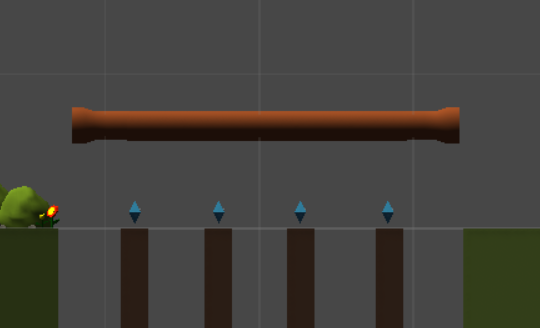
\includegraphics[width=\textwidth]{Grafiken/Weg_mit_vielen_Luecken.png}
		(a)
	\end{minipage}
	\begin{minipage}[b]{0.45\linewidth}
		\centering
		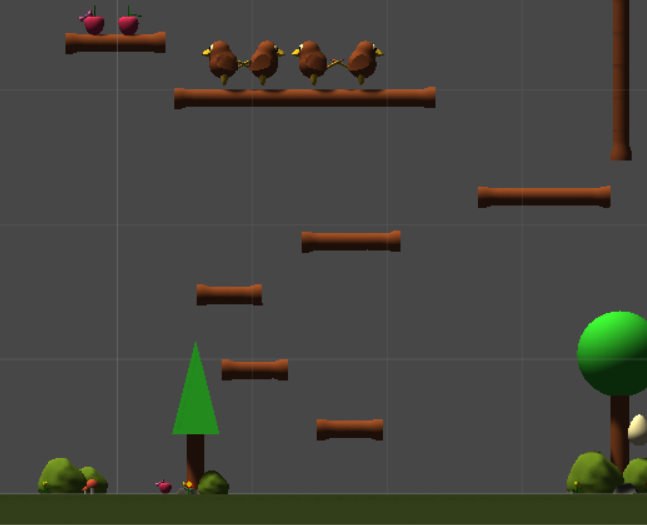
\includegraphics[width=\textwidth]{Grafiken/Kleine_Kirsche.png}
		(b)
	\end{minipage}
	\caption{2D-Ansicht des Weges mit den vielen L�cken (a) und der Szene mit der kleinen Kirsche (b)}
	\label{grafik: weg mit vielen l�cken kleine kirsche}
\end{figure}

\section{Die kleine Kirsche}

Im n�chsten Abschnitt (siehe Abbildung \ref{grafik: weg mit vielen l�cken kleine kirsche} (b)) befindet sich eine kleine Kirsche, deren Eltern von den V�geln verschleppt wurden, und die nun dringend Hilfe braucht. Um der Kirsche seine Hilfe anzubieten, muss der Spieler diese jedoch zun�chst ansprechen. Damit er diese M�glichkeit �berhaupt wahrnehmen kann, wird ihm von Antonio vorher erl�utert, dass er mit Hilfe einer bestimmten Taste andere Charaktere ansprechen kann. Au�erdem macht er darauf aufmerksam, dass die kleine Kirsche wom�glich Hilfe braucht. Bei diesem Test liegt der Fokus darauf, dass der Spieler Mitleid mit der Kleinen entwickeln soll. Daher muss, wenn er sie nicht anspricht, davon ausgegangen werden, dass er keines hat, weshalb dies einen Punkt Abzug auf diese Eigenschaft bedeutet. Ebenfalls einen Punkt Abzug bekommt er, wenn er die kleine Kirsche anspricht, aber ihre Bitte, die Eltern zu retten, ablehnt. Wenn dies passiert, wird sie au�erdem versuchen den Spieler durch Betteln umzustimmen. Wirkt dies nicht, gibt es einen zus�tzlichen Punkt Abzug auf Mitleid. Nur wenn der Spieler bei einer dieser beiden M�glichkeiten verspricht die Eltern zu retten und dies auch tut, kann er einen Punkt auf Mitleid bekommen. Da diese au�erdem von einer gro�en Menge Feinde bewacht werden, gibt es in diesem Fall auch einen Punkt auf Herausforderung.

\section{Die zerst�rbaren Bl�cke}

An dieser Stelle findet der Spieler eine Reihe zerst�rbarer Eier vor, zu denen Antonio ihm erkl�rt, dass sich in ihnen manchmal n�tzliche Gegenst�nde befinden und ihn auffordert diese zu zerbrechen. Kommt der Spieler dieser Aufforderung nach, gibt es sowohl einen Punkt auf die Sammlereigenschaft als auch einen Punkt Abzug auf Autonomie. Letzteres l�sst sich erneut auf dieselbe Art und Weise erkl�ren, wie schon bei dem ersten Diamanten und der Sprunganweisung, w�hrend Ersteres vergeben wird, da dies ein Hinweis darauf ist, dass sich der Spieler mit Hilfe von n�tzlichen Gegenst�nden, im Falle der zerbrechlichen Eier Diamanten, k�dern l�sst. Zerbricht der Spieler die Eier also nicht, erfolgt daher eine umgekehrte Punktevergabe.

\section{Die Diamanten am Abgrund}

Kurze Zeit sp�ter kommt der Spieler in die in Abbildung \ref{grafik: diamanten vor abgrund matschiger weg} (a) gezeigte Situation. Da es relativ aufwendig ist in die Einbuchtung mit den Diamanten zu gelangen, bringt die Entscheidung des Spielers, dies trotzdem zu tun, einen Punkt auf den Ehrgeiz und einen auf die Sammeleigenschaft. �berspringt er diese Stelle dahingegen einfach, gibt es auf beide Eigenschaften einen Punkt Abzug.

\begin{figure}[h]
	\centering
	\begin{minipage}[b]{0.45\linewidth}
		\centering
		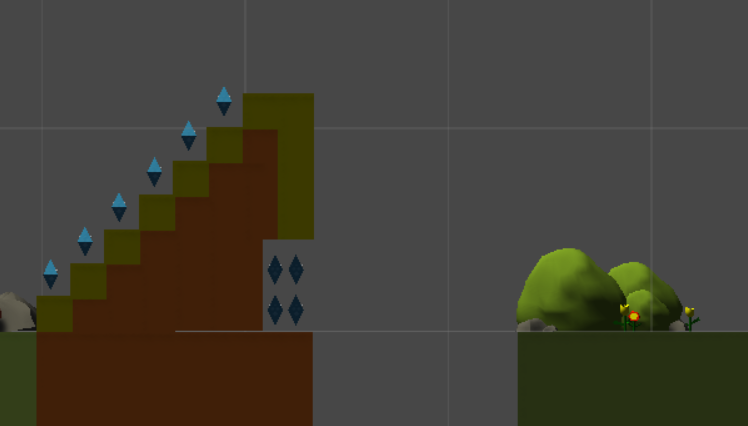
\includegraphics[width=\textwidth]{Grafiken/Abgrund_mit_Diamanten.png}
		(a)
	\end{minipage}
	\begin{minipage}[b]{0.45\linewidth}
		\centering
		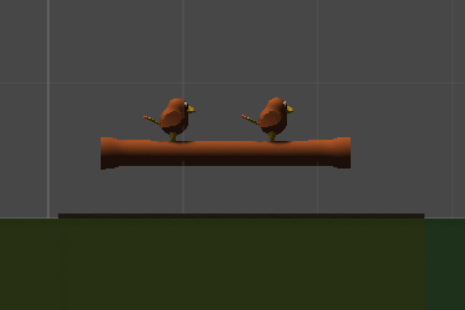
\includegraphics[width=\textwidth]{Grafiken/Matschiger_Weg.png}
		(b)
	\end{minipage}
	\caption{Ansicht der Schr�ge vor dem Abgrund zusammen mit der Einbuchtung, die die Diamanten enth�lt (a) und des Abschnittes mit dem matschigen Weg in 2D (b)}
	\label{grafik: diamanten vor abgrund matschiger weg}
\end{figure}

\section{Der matschige Weg}

Nach dem �berqueren des Abgrunds gelangt der Spieler an die durch Abbildung \ref{grafik: diamanten vor abgrund matschiger weg} (b) dargestellte Stelle. Der untere Weg erfordert dabei viel Geduld, da er mit einem matschigen Boden �berzogen ist, der den Spieler sehr viel langsamer macht. Aus diesem Grund erh�lt er einen Punkt auf Geduld, sollte er sich daf�r entscheiden diesen den oben patrouillierenden V�geln vorzuziehen. Allerdings resultiert daraus auch ein Punkt Abzug auf Herausforderung. Durch die Platzierung der V�gel sollte hier f�r den entsprechenden Spielertypen auch genau dieser Anreiz gegeben werden, da es ohne diese gar keinen Grund geben w�rde den langsameren, unteren Weg zu nehmen. Spieler, die sich dahingegen daf�r entscheiden lieber die V�gel zu besiegen, um schneller zu sein, bekommen hierf�r sowohl einen Punkt auf Herausforderung als auch einen Abzug auf Geduld.

\section{Die gl�nzenden, zerbrechliche Bl�cke}

Der kommende Abschnitt h�lt ebenfalls die bereits bekannten, zerbrechlichen Eier bereit. Einige von diesen gl�nzen nun, um die Aufmerksamkeit des Spielers zu pr�fen. So bekommt er einen Punkt auf das Merkmal Aufmerksamkeit, wenn er diese zerst�rt und entsprechend einen Punkt Abzug, wenn er dies nicht tut. Diese Art Test tritt au�erdem noch einmal am Ende des Analyse-Levels auf.

\section{Der bewegliche Baumstamm �ber dem Abgrund}

Abbildung \ref{grafik: beweglicher baumstamm gef�hrliche grube} (a) zeigt eine Stelle, an der der Spieler nochmals auf Geduld und Ehrgeiz getestet werden soll. Bringt er auf dem unteren Weg die Geduld auf mit dem beweglichen Baumstamm langsam �ber den Abgrund zu fahren und umgeht somit den steuerungstechnisch schwereren, oberen Weg, erh�lt er nicht nur einen Punkt auf Geduld, sondern auch einen Punkt Abzug auf die Eigenschaft Ehrgeiz. Umgekehrt gibt es einen Punkt auf Ehrgeiz und einen Abzug auf Geduld.

\begin{figure}[h]
	\centering
	\begin{minipage}[b]{0.45\linewidth}
		\centering
		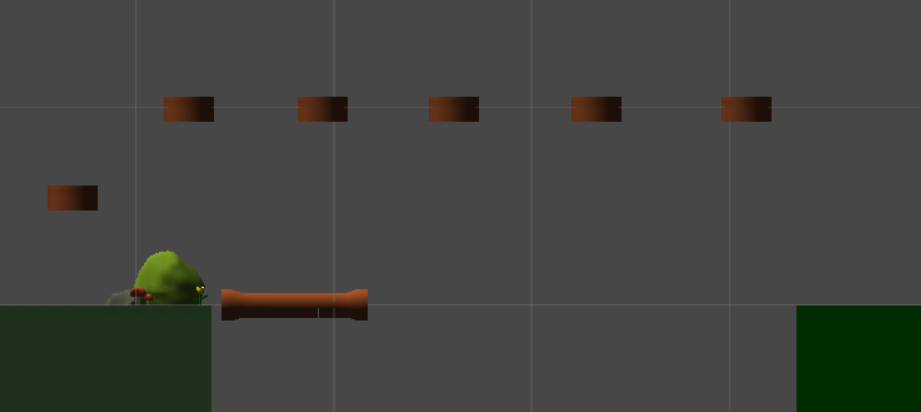
\includegraphics[width=\textwidth]{Grafiken/Beweglicher_Baumstamm_ueber_Abgrund.png}
		(a)
	\end{minipage}
	\begin{minipage}[b]{0.45\linewidth}
		\centering
		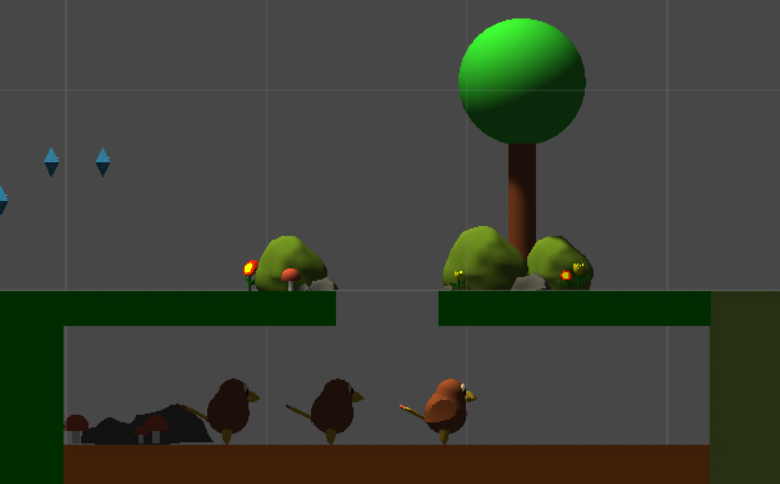
\includegraphics[width=\textwidth]{Grafiken/Gefaehrliche_Grube.png}
		(b)
	\end{minipage}
	\caption{2D-Ansicht des Abgrundes mit dem beweglichen Baumstamm (a) und der unterirdischen Grube, in der es viele Feinde zu besiegen gibt (b)}
	\label{grafik: beweglicher baumstamm gef�hrliche grube}
\end{figure}

\section{Die gef�hrliche Grube}

An diesem Punkt (siehe Abbildung \ref{grafik: beweglicher baumstamm gef�hrliche grube} (b)) angekommen, kann der Spieler sich in eine unter der Erde befindliche Grube begeben, um dort viele Gegner zu besiegen. Tut er dies, bekommt er somit einen Punkt auf Herausforderung, w�hrend er im umgekehrten Fall einen Punkt Abzug auf dieses Merkmal erh�lt.

\section{Die Geduldsprobe mit den V�geln}

Eine weitere Geduldsprobe (dargestellt in Abbildung \ref{grafik: unsichtbarer weg geduldsprobe kirsche in not} (a)) erwartet den Spieler schlie�lich in Form langsam unter einem Baumstamm herannahender Feinde, die erst besiegt werden k�nnen, wenn sie unter diesem hervorkommen. Wartet der Spieler auf diesen Moment, um die V�gel zu besiegen, gibt es daher einen Punkt auf Herausforderung und einen auf Geduld. Andernfalls erh�lt er auf beide Merkmale einen Punkt Abzug. 

\section{Der unsichtbare Weg}

Auch in Abbildung \ref{grafik: unsichtbarer weg geduldsprobe kirsche in not} (a) dargestellt, ist ein zu vielen Diamanten nach oben f�hrender Weg, der f�r den Spieler erst sichtbar wird, wenn er von unten gegen die schmalen, ebenfalls noch unsichtbaren, Bl�cke springt. In diesem Fall gibt es einen Punkt auf Aufmerksamkeit, da die Idee dem Spieler nur kommen kann, wenn er auf das am Anfang des Weges befindliche Schild mit dem Pfeil darauf geachtet hat. Erklimmt er diesen Weg nicht, gibt es einen Punkt Abzug auf die Eigenschaft Aufmerksamkeit.

\begin{figure}[h]
	\centering
	\begin{minipage}[b]{0.45\linewidth}
		\centering
		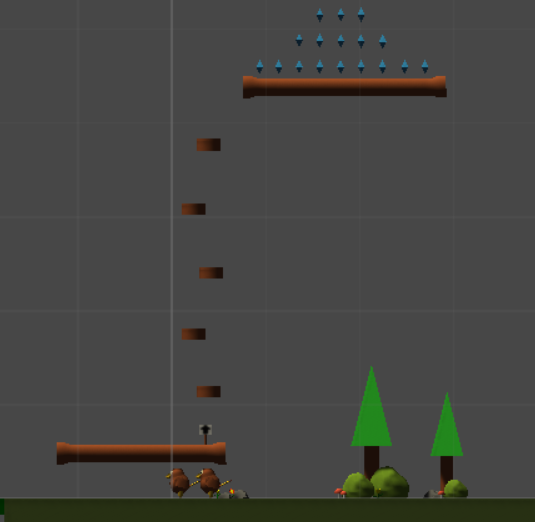
\includegraphics[width=\textwidth]{Grafiken/Unsichtbarer_Weg_Geduldsprobe_Voegel.png}
		(a)
	\end{minipage}
	\begin{minipage}[b]{0.45\linewidth}
		\centering
		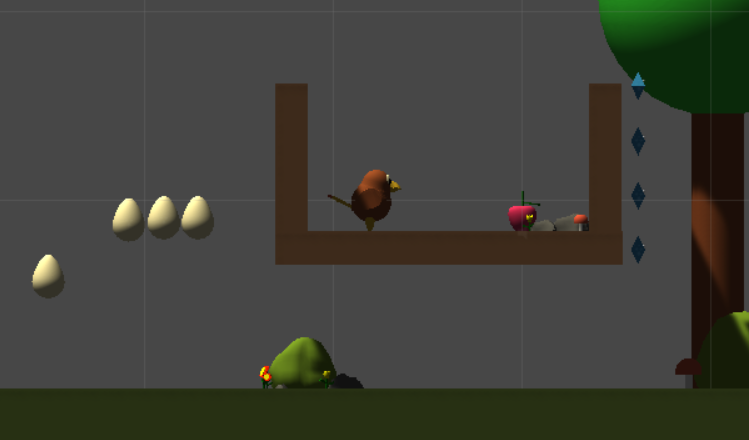
\includegraphics[width=\textwidth]{Grafiken/U_foermige_Einbuchtung_mit_Kirsche.png}
		(b)
	\end{minipage}
	\caption{Szene f�r die Geduldsprobe und den unsichtbaren Weg (a) sowie f�r die in Not geratene Kirsche in 2D (b)}
	\label{grafik: unsichtbarer weg geduldsprobe kirsche in not}
\end{figure}

\section{Die in Not geratene Kirsche}

In dieser Szene (siehe Abbildung \ref{grafik: unsichtbarer weg geduldsprobe kirsche in not} (b)) bekommt der Spieler den Schrei einer durch einen Vogel bedrohte Kirsche zu h�ren. Hat er daraufhin Mitleid und eilt ihr zu Hilfe, erh�lt er einen Punkt auf die Eigenschaft Mitleid, w�hrend das Ignorieren der Kirsche zu einem Punkt Abzug auf dieses Merkmal f�hrt.

\chapter{Abbildungen}
\label{chap:anhang_abbildungen}
\hideInContents
% Abbildung: Screenshots
\section{Screenshots}
%---------------------------------------------------------------------------------------------------------------------
\subsection{Hauptmen�}
\begin{figure}[H]
	\begin{center}
		\fbox{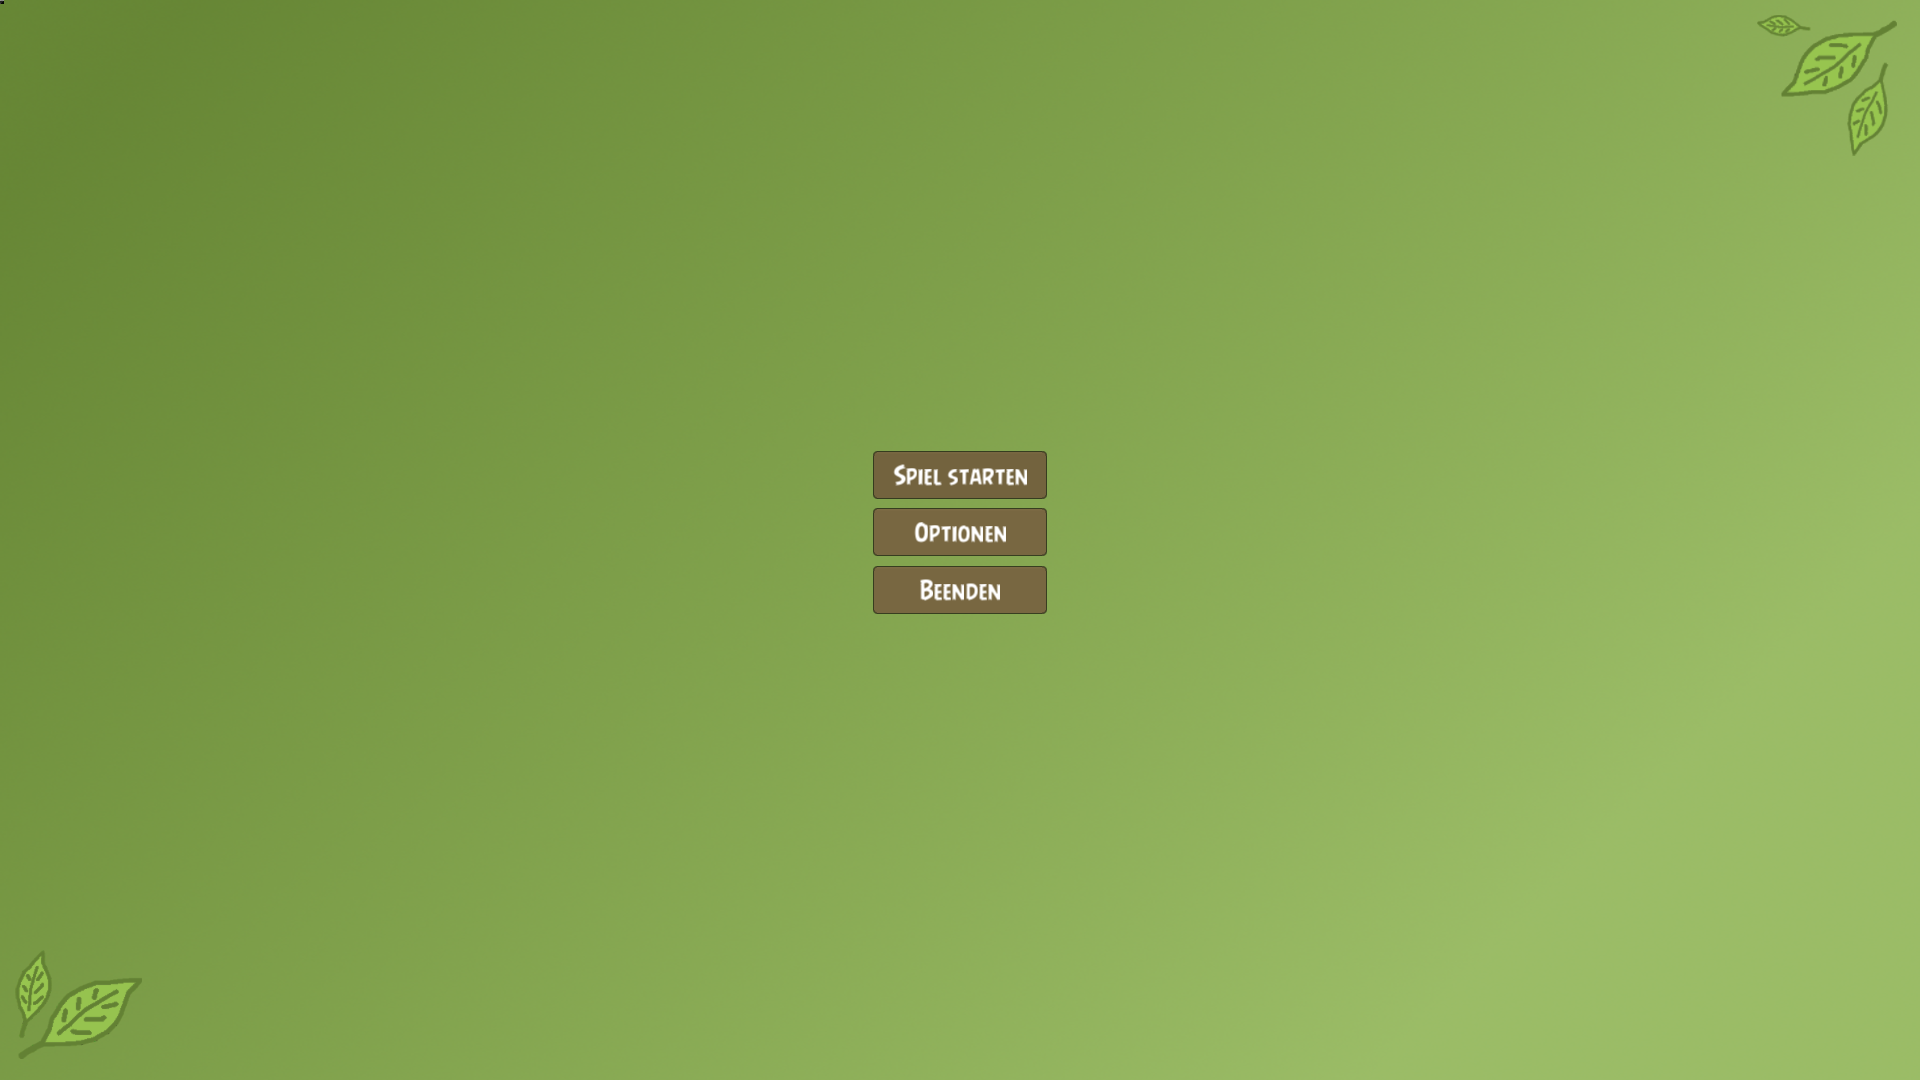
\includegraphics[page=1,width=0.98\linewidth]{Inhalt/Anhang/Screenshots/screenshot_0.png}}
	\end{center}	
	\caption[Hauptmen�]{Hauptmen� (Eigene Darstellung)}
	\label{fig:anhang_screenshots_menu}
\end{figure}
%---------------------------------------------------------------------------------------------------------------------
\subsection{Analyse--Level}
\begin{figure}[H]
	\begin{center}
		\fbox{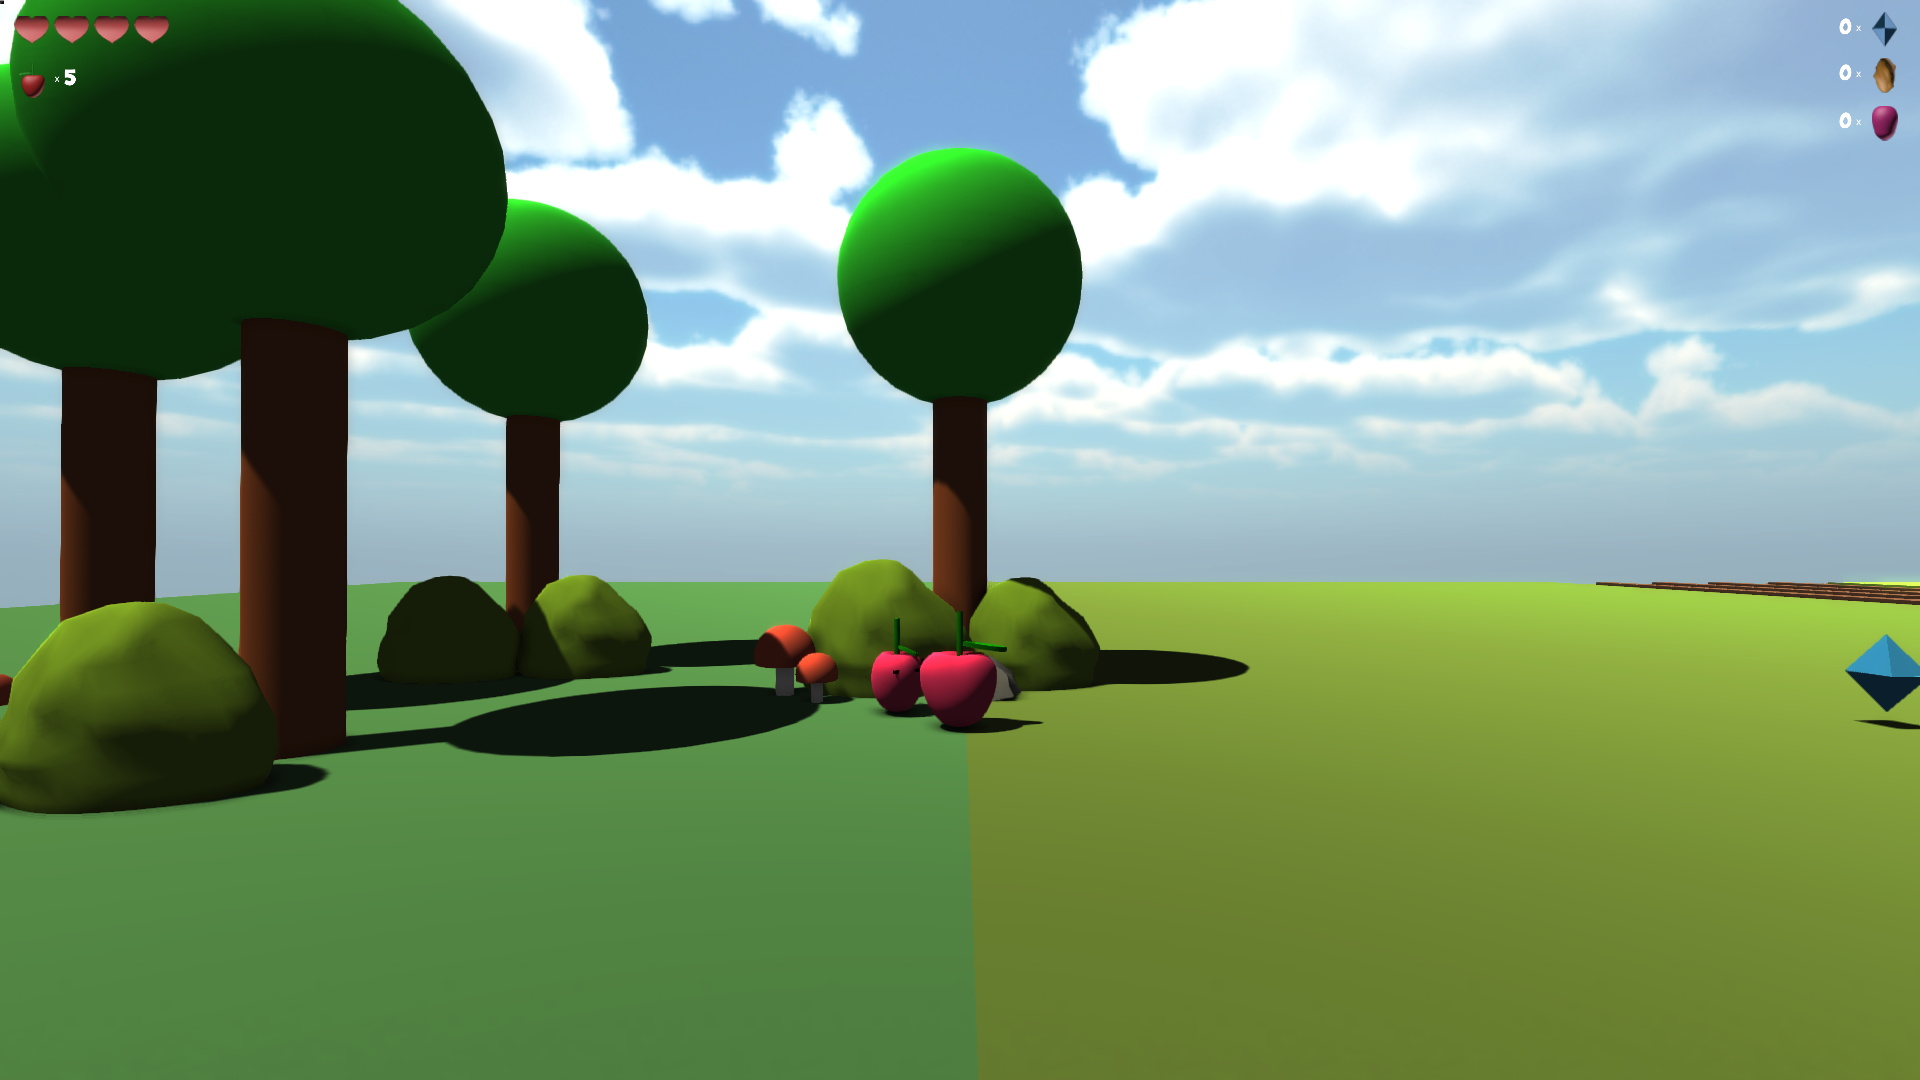
\includegraphics[page=1,width=0.98\linewidth]{Inhalt/Anhang/Screenshots/screenshot_1.png}}
	\end{center}	
	\caption[Am Fu�e des Baums]{Am Fu�e des Baums (Eigene Darstellung)}
	\label{fig:anhang_screenshots_level1_baum}
\end{figure}
%
\begin{figure}[H]
	\begin{center}
		\fbox{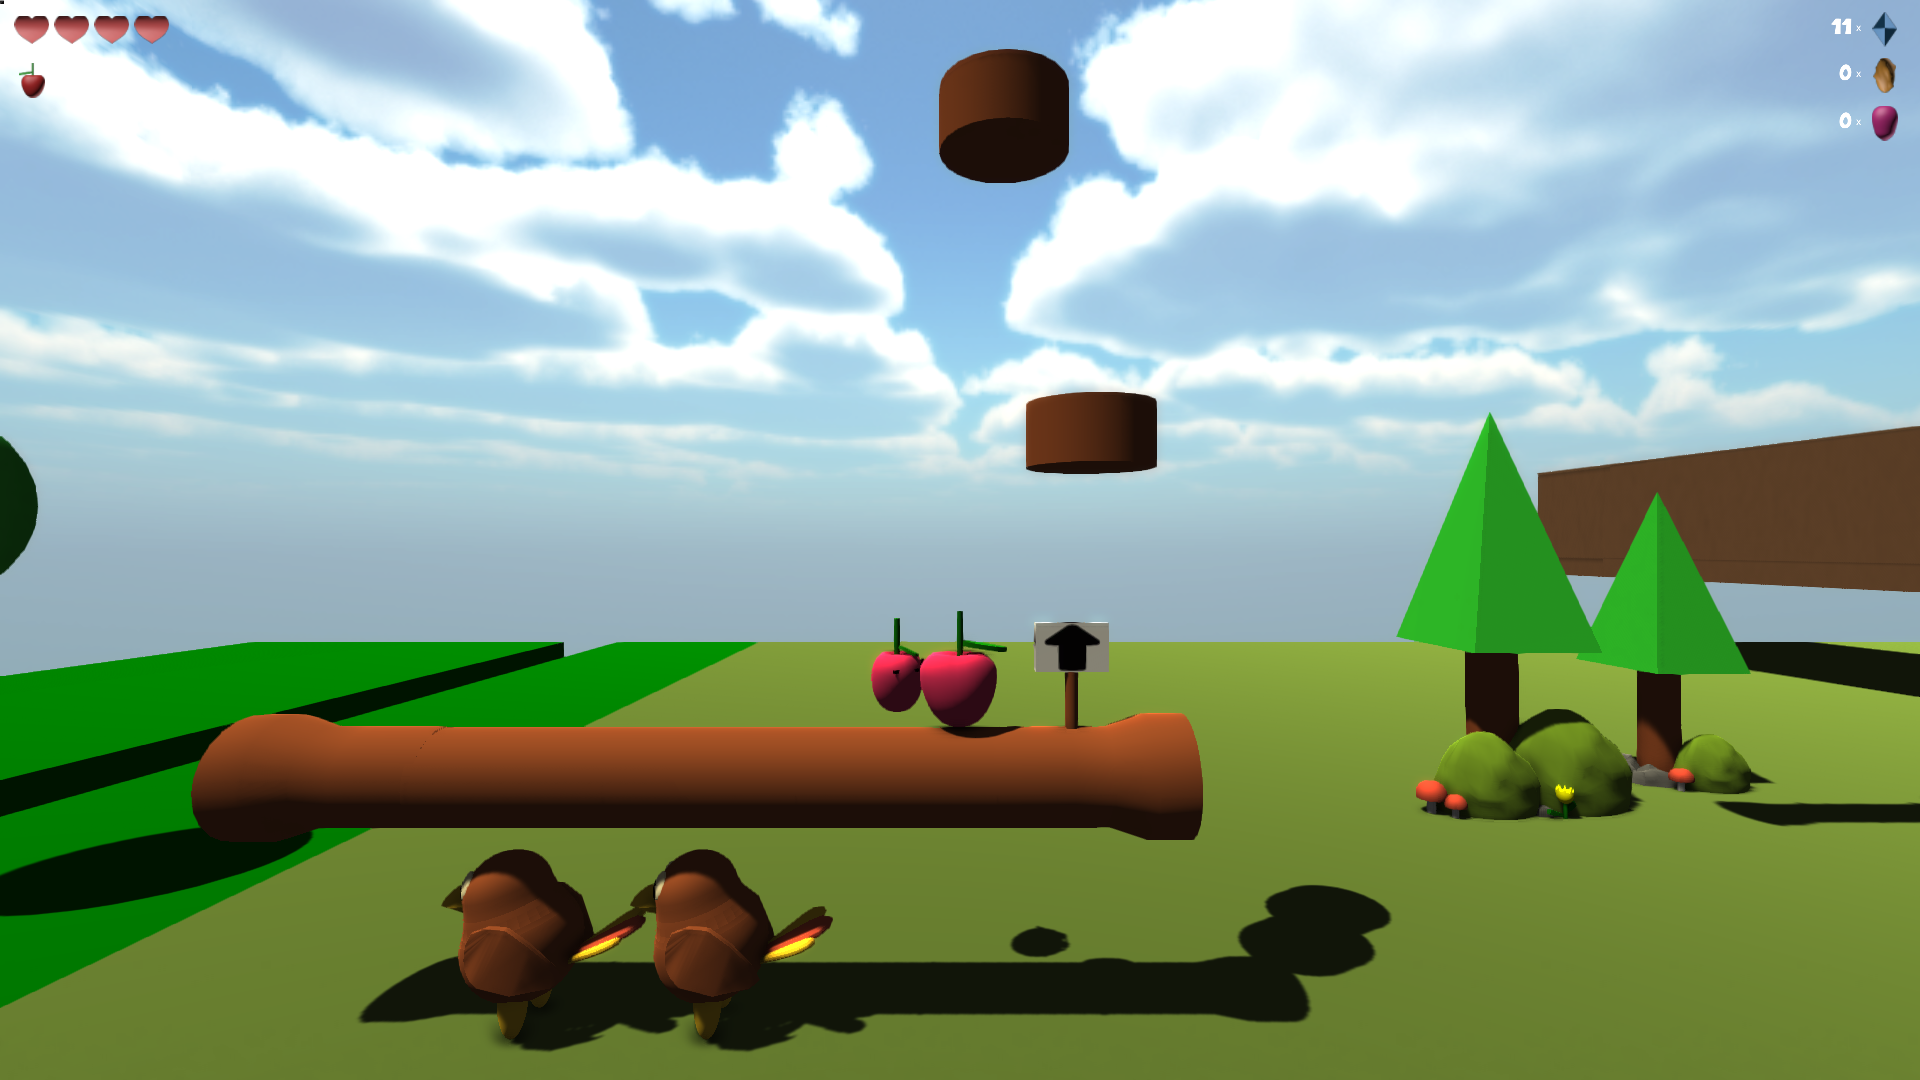
\includegraphics[page=1,width=0.98\linewidth]{Inhalt/Anhang/Screenshots/screenshot_4.png}}
	\end{center}	
	\caption[Versteckter Weg]{Versteckter Weg (Eigene Darstellung)}
	\label{fig:anhang_screenshots_level1_weg}
\end{figure}
%---------------------------------------------------------------------------------------------------------------------
\subsection{Der kaputte Brunnen}
\begin{figure}[H]
	\begin{center}
		\fbox{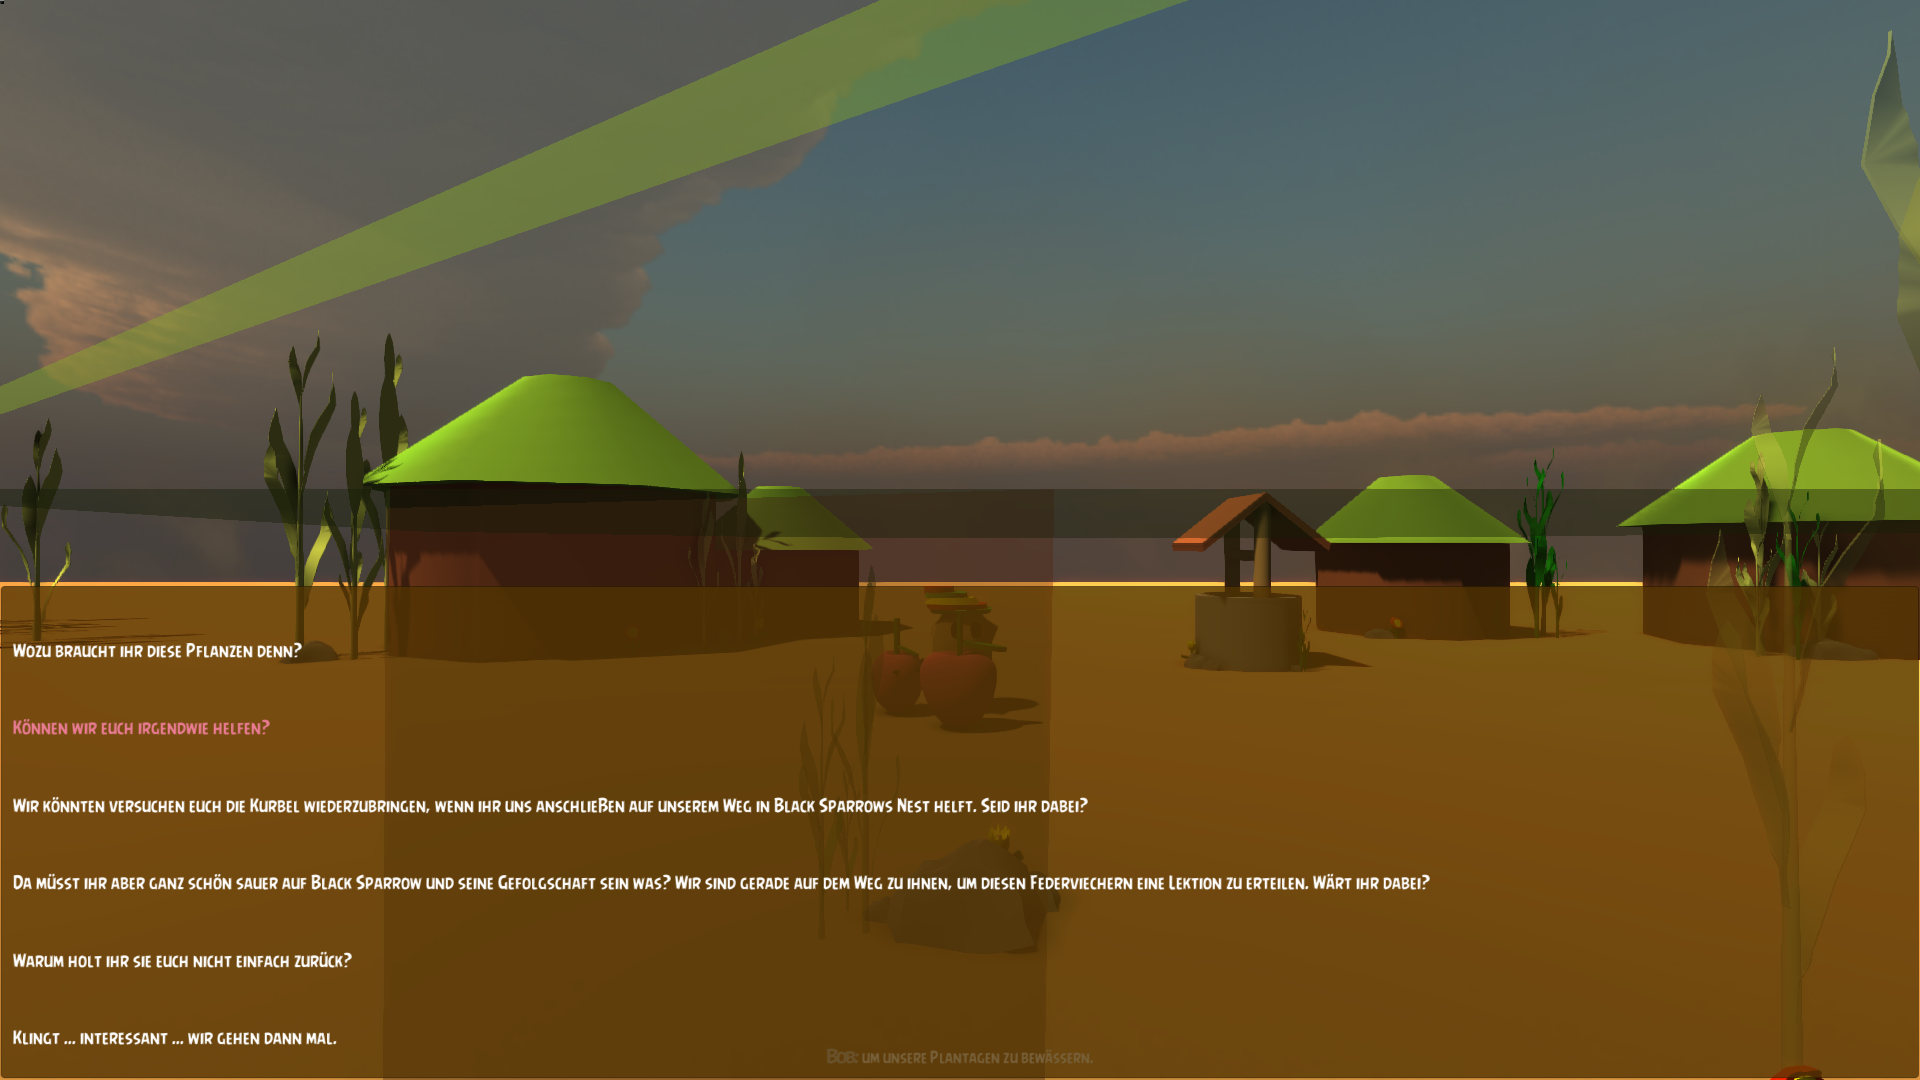
\includegraphics[page=1,width=0.98\linewidth]{Inhalt/Anhang/Screenshots/screenshot_8.png}}
	\end{center}	
	\caption[Unterhaltung mit Bob]{Unterhaltung mit Bob (Eigene Darstellung)}
	\label{fig:anhang_screenshots_level2_bob}
\end{figure}
\begin{figure}[H]
	\begin{center}
		\fbox{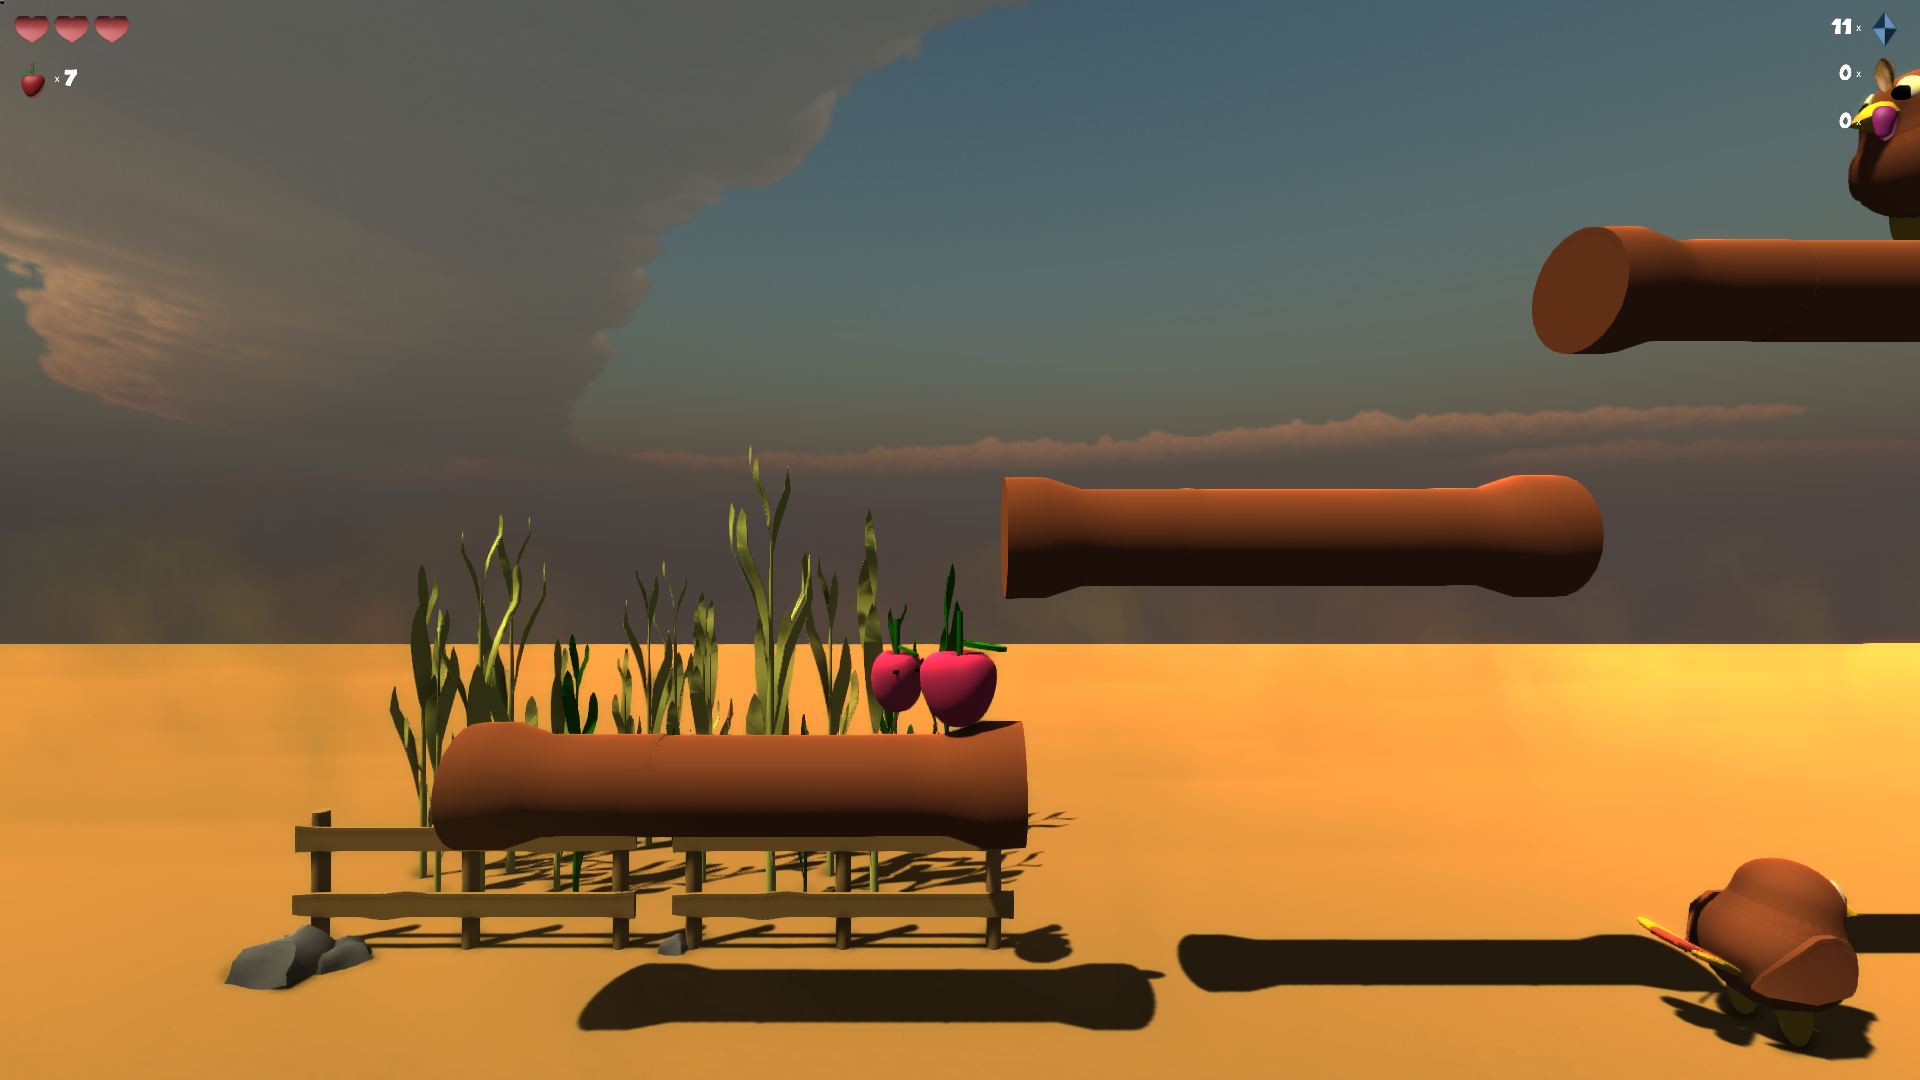
\includegraphics[page=1,width=0.98\linewidth]{Inhalt/Anhang/Screenshots/screenshot_9.png}}
	\end{center}	
	\caption[Pfad mit Hindernissen]{Pfad mit Hindernissen (Eigene Darstellung)}
	\label{fig:anhang_screenshots_level2_hindernisse}
\end{figure}
\begin{figure}[H]
	\begin{center}
		\fbox{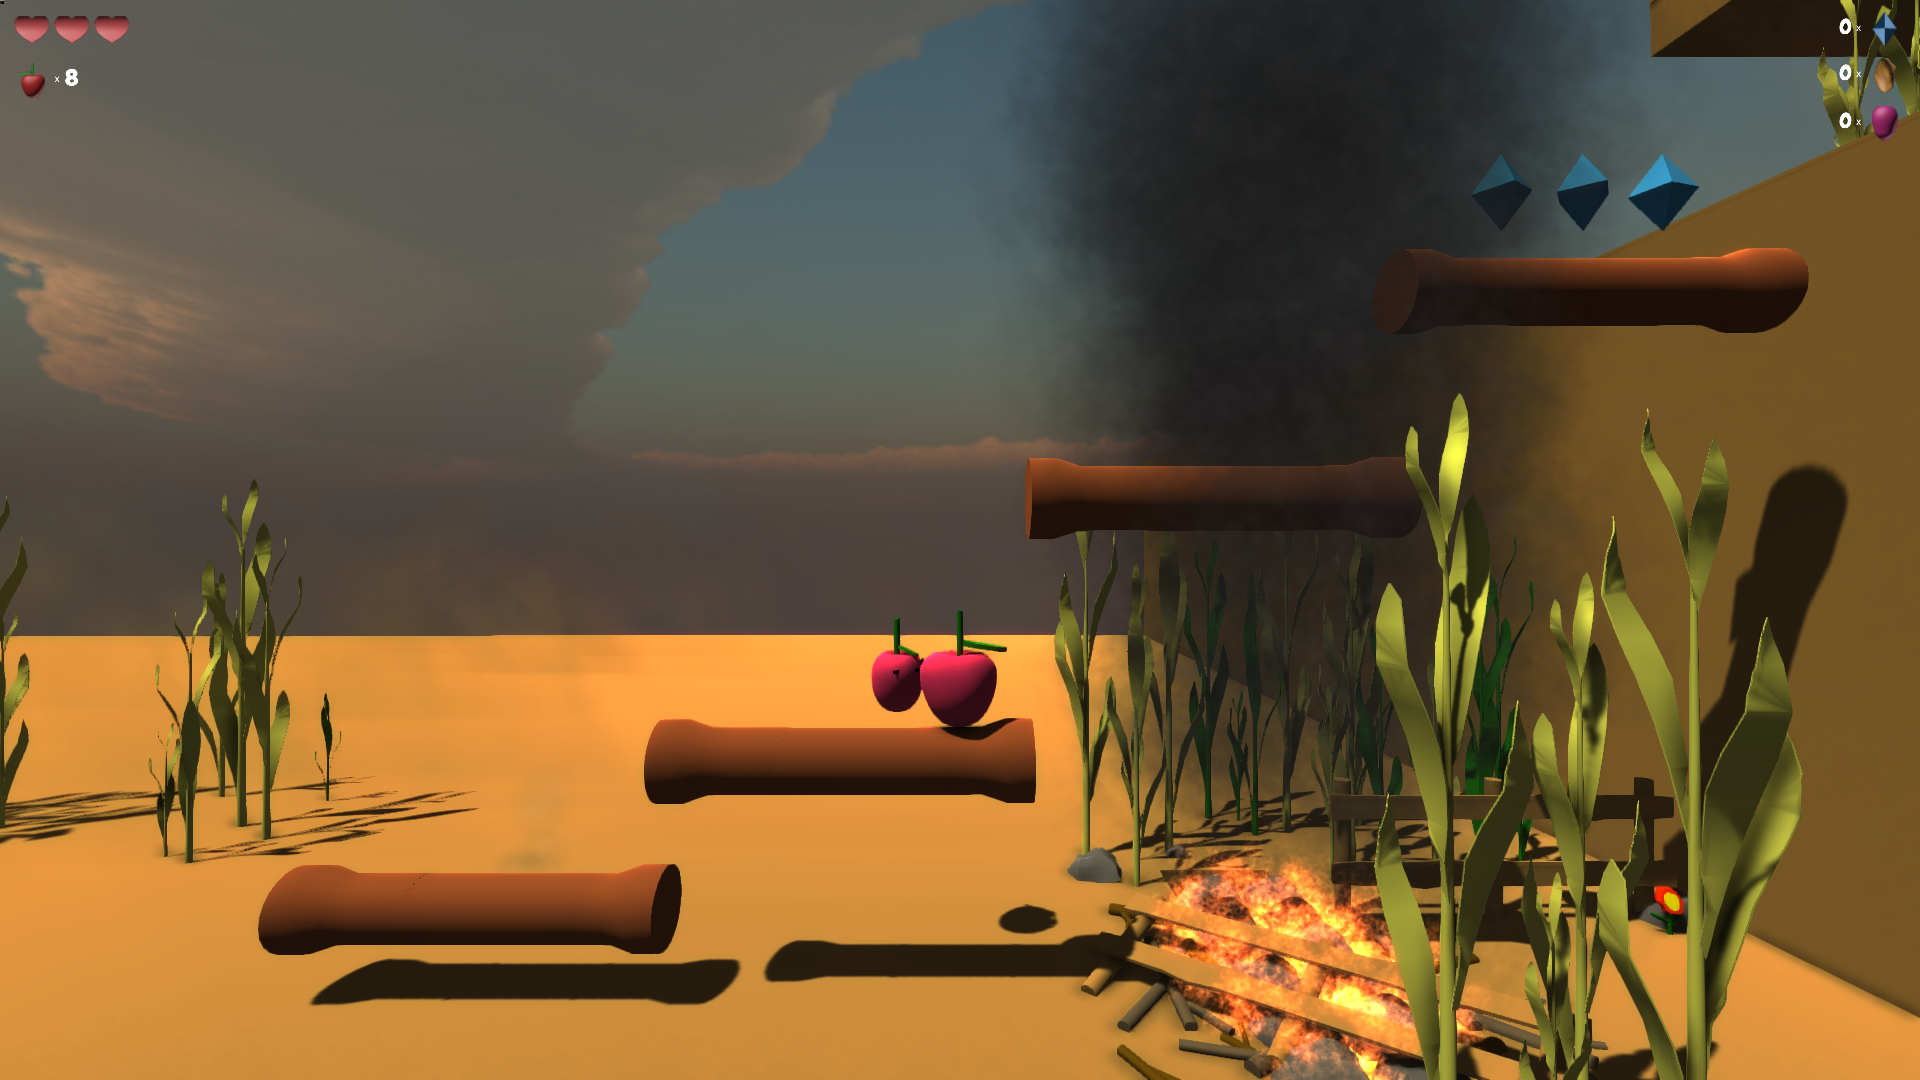
\includegraphics[page=1,width=0.98\linewidth]{Inhalt/Anhang/Screenshots/screenshot_12.png}}
	\end{center}	
	\caption[Eingest�rzte H�hle]{Eingest�rzte H�lle (Eigene Darstellung)}
	\label{fig:anhang_screenshots_level2_hoehle}
\end{figure}
%---------------------------------------------------------------------------------------------------------------------
\subsection{Der dunkle Wald} 
\begin{figure}[H]
	\begin{center}
		\fbox{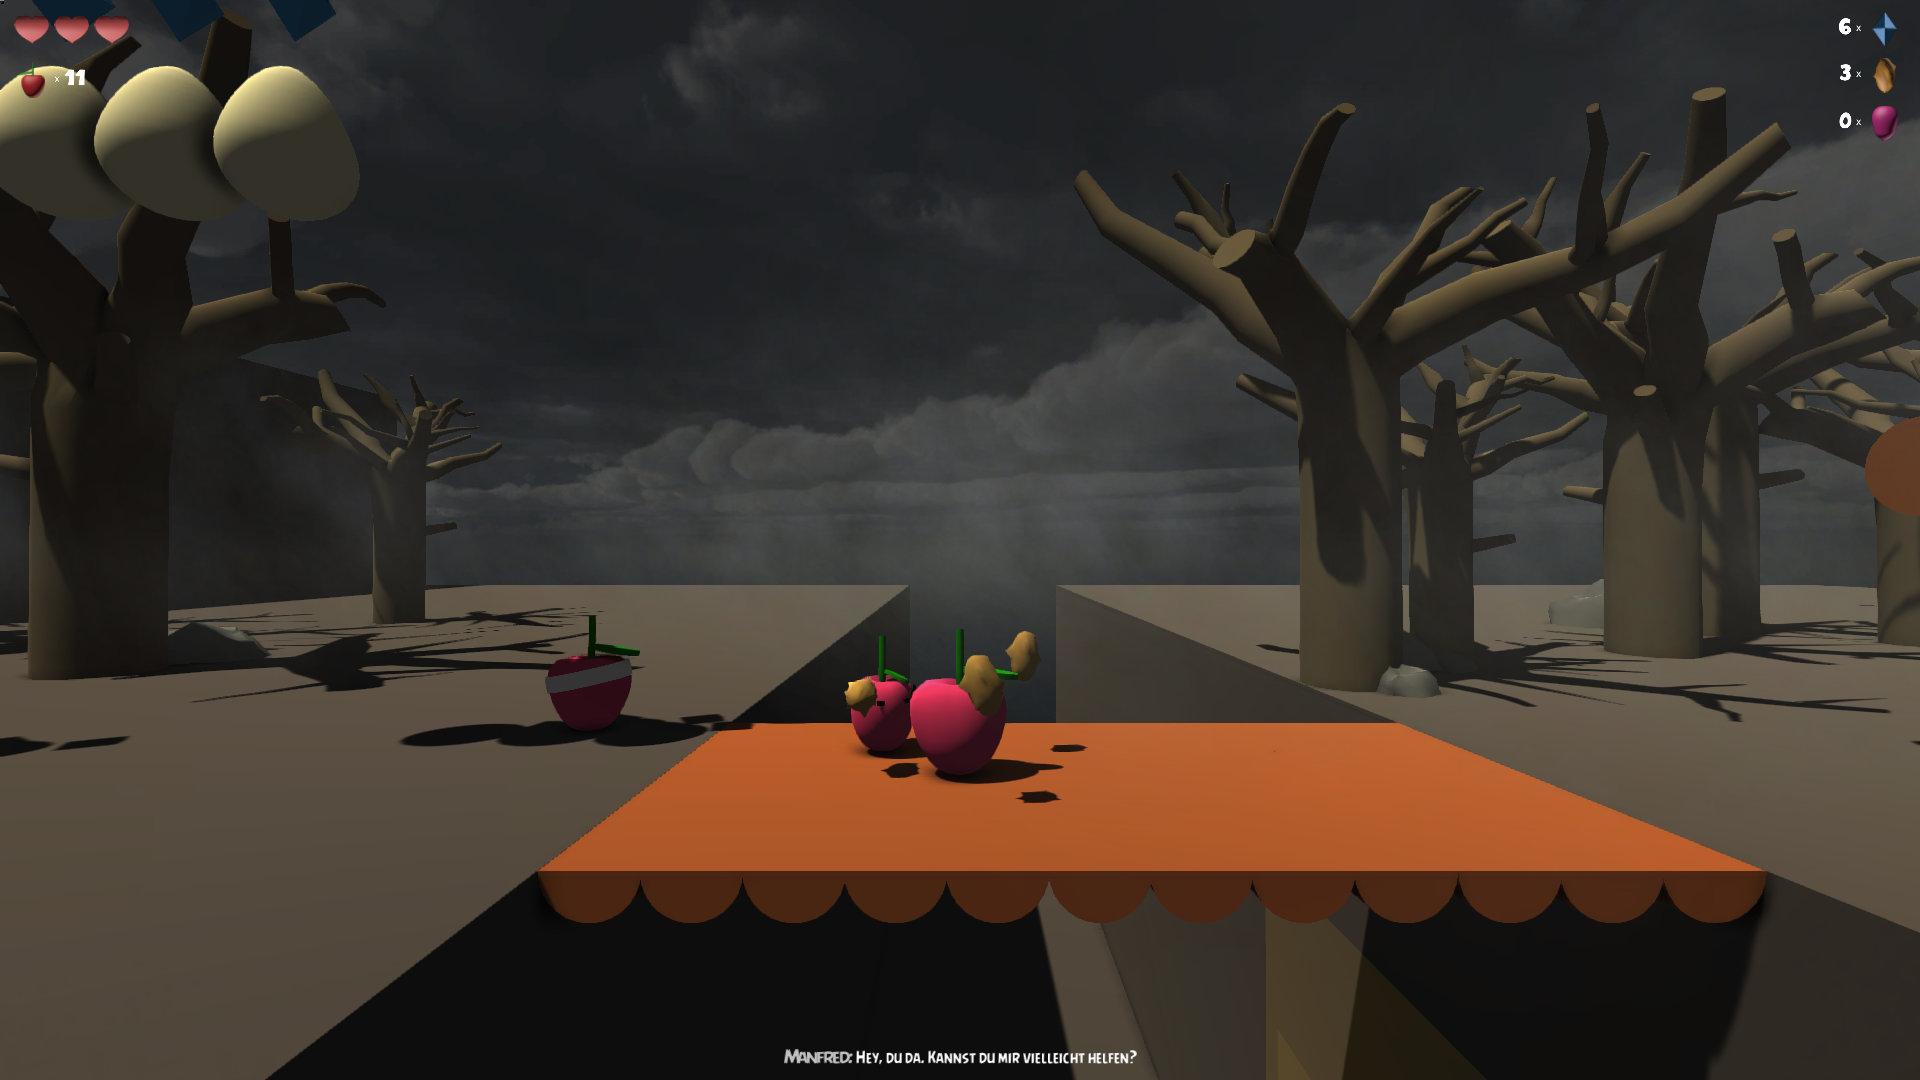
\includegraphics[page=1,width=0.98\linewidth]{Inhalt/Anhang/Screenshots/screenshot_22.png}}
	\end{center}	
	\caption[Unterhaltung mit Manfred]{Unterhaltung mit Manfred (Eigene Darstellung)}
	\label{fig:anhang_screenshots_level3_manfred}
\end{figure}
\begin{figure}[H]
	\begin{center}
		\fbox{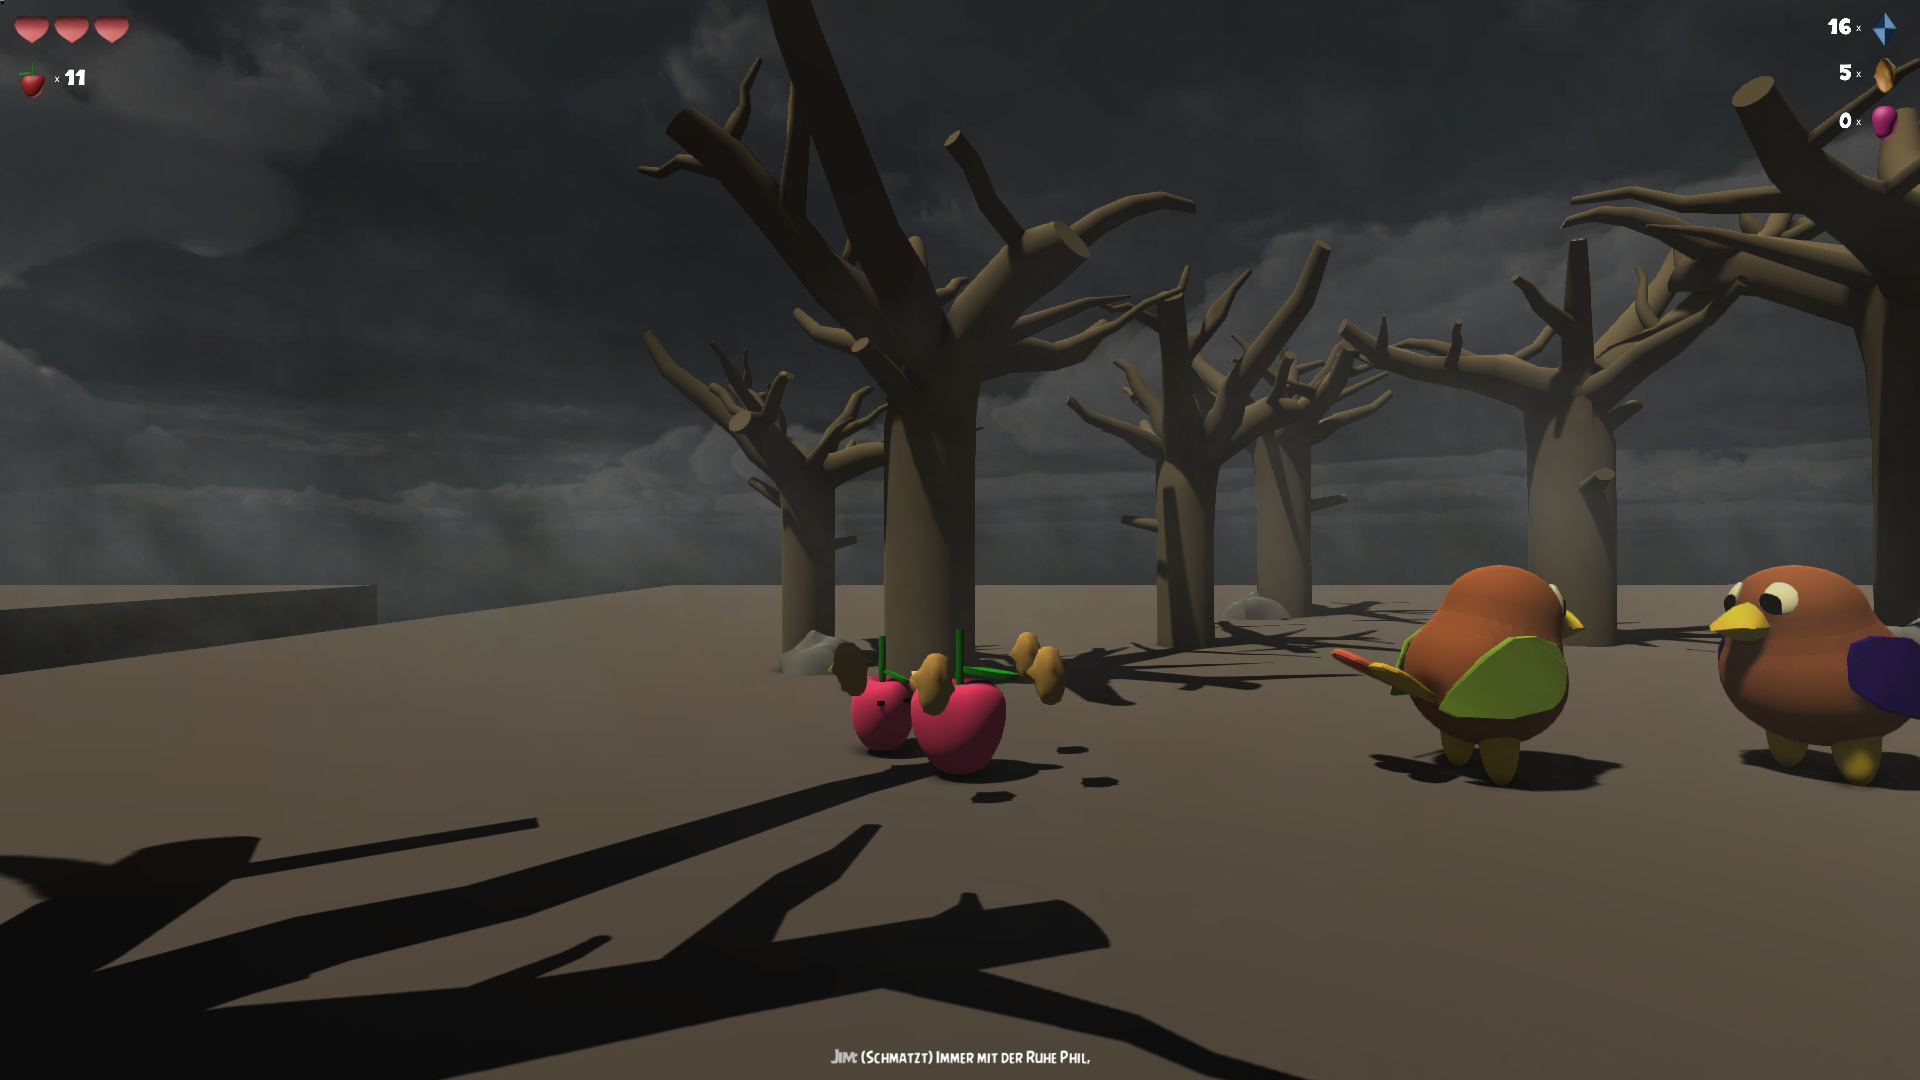
\includegraphics[page=1,width=0.98\linewidth]{Inhalt/Anhang/Screenshots/screenshot_24.png}}
	\end{center}	
	\caption[Verfolgung der Handlanger]{Verfolgung der Handlanger (Eigene Darstellung)}
	\label{fig:anhang_screenshots_level3_verfolgung}
\end{figure}
%---------------------------------------------------------------------------------------------------------------------
\subsection{Black Sparrows Nest}
\begin{figure}[H]
	\begin{center}
		\fbox{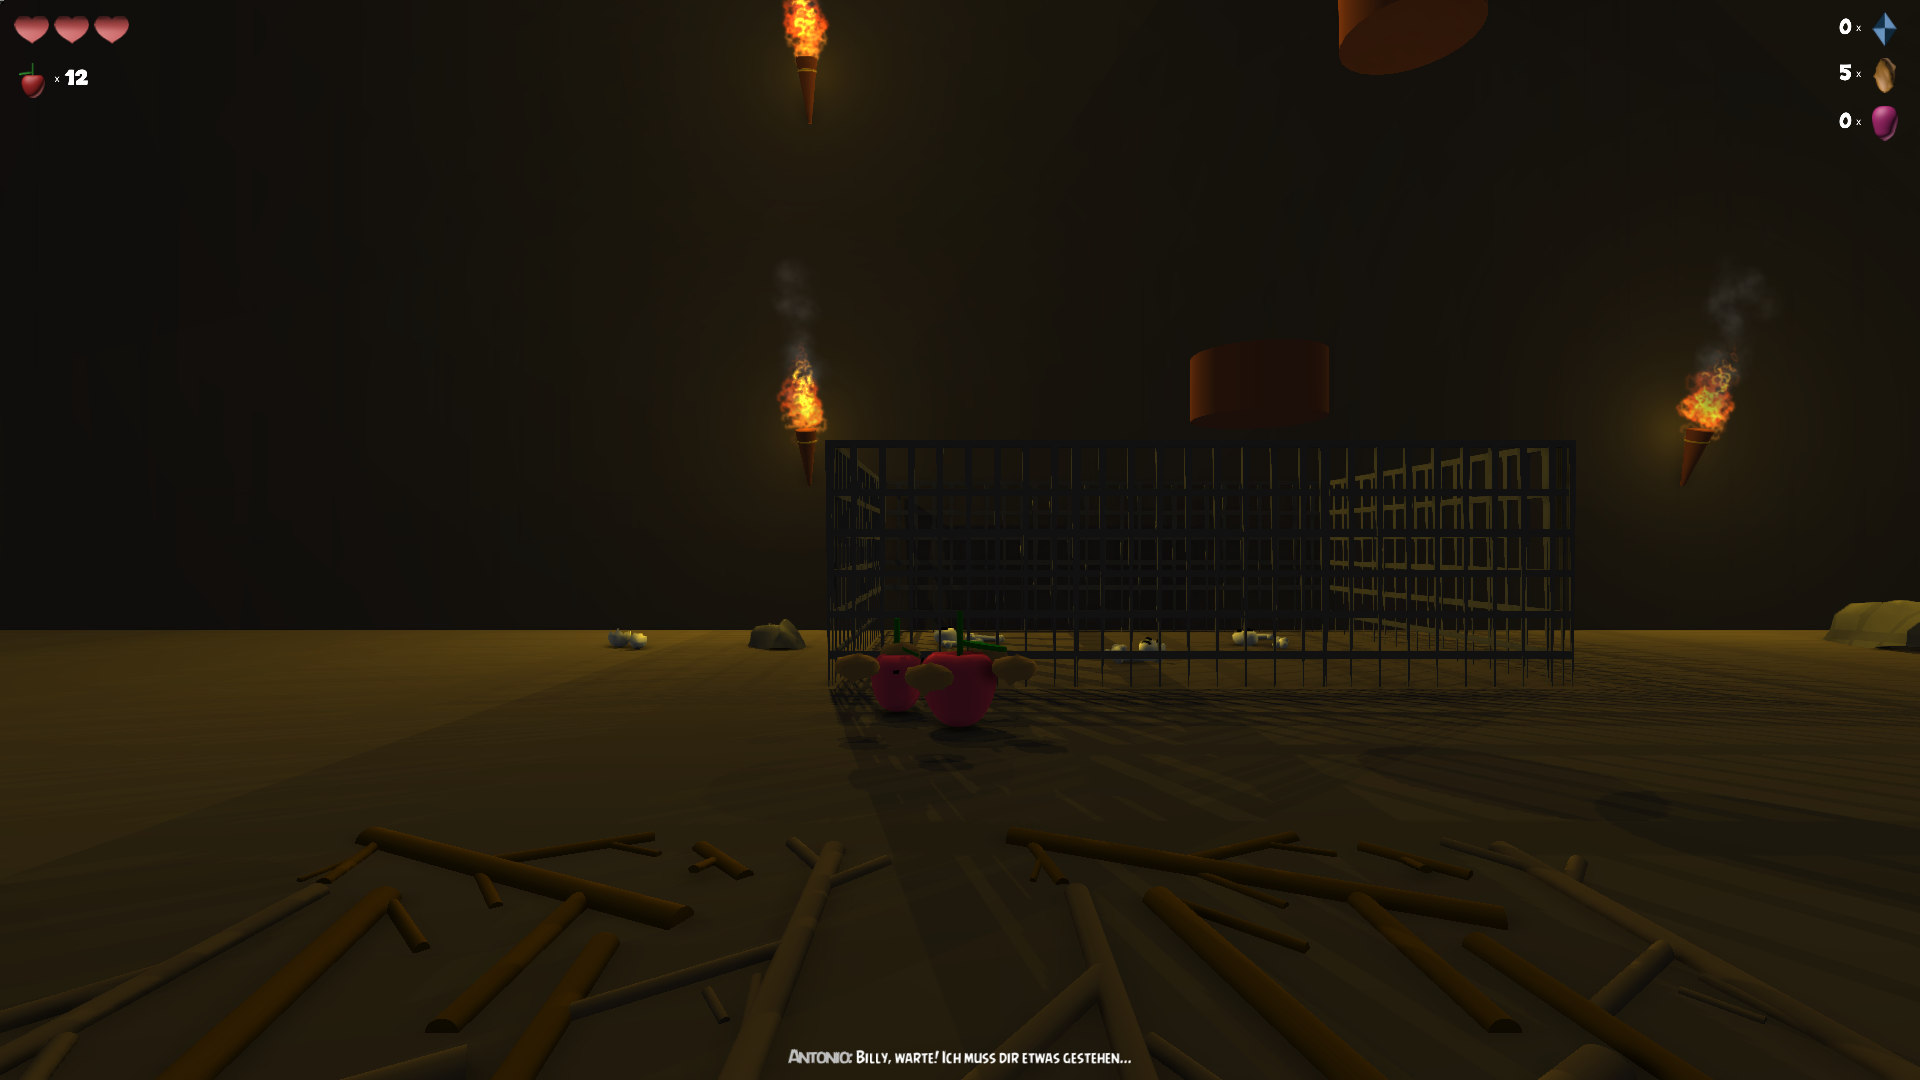
\includegraphics[page=1,width=0.98\linewidth]{Inhalt/Anhang/Screenshots/screenshot_30.png}}
	\end{center}	
	\caption[Antonios Gest�ndnis]{Antonios Gest�ndnis (Eigene Darstellung)}
	\label{fig:anhang_screenshots_level32_antonio}
\end{figure}
\showInContents	
\end{appendices}								% Anhang einbinden	
\end{document}